% !Mode:: "TeX:UTF-8"
%%%%%%%%%%%%%%%%%%%%%%%%%%%%%%%%%%%%%%%%%%%%%%%%%%%%%%%%%%%%%%%%%%%%%%%%%%%%%%%%
%          ,
%      /\^/`\
%     | \/   |                CONGRATULATIONS!
%     | |    |             SPRING IS IN THE AIR!
%     \ \    /                                                _ _
%      '\\//'                                               _{ ' }_
%        ||                     hithesis v3                { `.!.` }
%        ||                                                ',_/Y\_,'
%        ||  ,                   dustincys                   {_,_}
%    |\  ||  |\          Email: yanshuoc@gmail.com             |
%    | | ||  | |            https://yanshuo.name             (\|  /)
%    | | || / /                                               \| //
%    \ \||/ /       https://github.com/dustincys/hithesis      |//
%      `\\//`   \\   \./    \\ /     //    \\./   \\   //   \\ |/ /
%     ^^^^^^^^^^^^^^^^^^^^^^^^^^^^^^^^^^^^^^^^^^^^^^^^^^^^^^^^^^^^^^
%%%%%%%%%%%%%%%%%%%%%%%%%%%%%%%%%%%%%%%%%%%%%%%%%%%%%%%%%%%%%%%%%%%%%%%%%%%%%%%%
% \documentclass[fontset=fandol,type=master,campus=shenzhen]{hithesisbook}
\documentclass[fontset=fandol,tocblank=false,type=master,campus=shenzhen,engtoc=false,absupper=true,newgeometry=two]{hithesisbook}
% 此处选项中不要有空格
%%%%%%%%%%%%%%%%%%%%%%%%%%%%%%%%%%%%%%%%%%%%%%%%%%%%%%%%%%%%%%%%%%%%%%%%%%%%%%%%
% 必填选项 
% type=doctor|master|bachelor|postdoc
%%%%%%%%%%%%%%%%%%%%%%%%%%%%%%%%%%%%%%%%%%%%%%%%%%%%%%%%%%%%%%%%%%%%%%%%%%%%%%%%
% 选填选项(选填选项的缺省值已经尽可能满足了大多数需求,除非明确知道自己有什么
% 需求)
% campus=shenzhen|weihai|harbin
%   含义:校区选项,默认harbin
% glue=true|false
%   含义:由于我工规范中要求字体行距在一个闭区间内,这个选项为true表示tex自
%   动选择,为false表示区间内一个最接近版心要求行数的要求的默认值,缺省值为
%   false。
% tocfour=true|false
%   含义:是否添加第四级目录,只对本科文科个别要求四级目录有效,缺省值为
%   false
% fontset=windows|mac|ubuntu|fandol|adobe
%   含义:设置字体,默认情况会自动识别系统,然后设置字体。后两个是开源字体,自行
%   下载安装后设置使用。windows是中易字库,窝工默认常用字体,绝对没毛病。mac和
%   ubuntu 默认分别是华文和思源字库,理论上用什么字库都行。后两种开源字库的安装
%   方法到谷歌上百度一下什么都有了。Linux非ubuntu发行版、非x86架构机器等如何运行
%   可到github issue上讨论。
% tocblank=true|false
%   含义:目录中第一章之前,是否加一行空白。缺省值为true。
% chapterhang=true|false
%   含义:目录的章标题是否悬挂居中,规范中要求章标题少于15字,所以这个选项
%   有无没什么用,除了特殊需求。缺省值为true。
% fulltime=true|false
%   含义:是否全日制,缺省值为true。非全日制如同等学力等,要在cover中设置类
%   型,封面中不同格式
% subtitle=true|false
%   含义:论文题目是否含有副标题,缺省值为false,如果有要在cover中设置副标
%   题内容,封面中显示。
% newgeometry=one|two
%   含义:规范中的自相矛盾之处,版芯是否包含页眉页脚,旧方法是按照包含页眉
%   页脚来设置。该选项是多选选项,如果没有这个选项,缺省值是旧模板的版芯设
%   置方法,如果设置该选项one或two,分别对应两种页眉页码对应版芯线的相对位
%   置。第一种是严格按照规范要求,难看。第二种微调了页眉页码位置,好一点。
% debug=true|false
%   含义:是否显示版芯框和行号,用来调试。默认否。
% openright=true|false
%   含义:博士论文是否要求章节首页必须在奇数页,此选项不在规范要求中,按个
%   人喜好自行决定。 默认否。注意,窝工的默认情况是打印版博士论文要求右翻页
%   ,电子版要求非右翻页且无空白页。如果想DIY(或身不由己DIY)在什么地方右
%   翻页,将这个选项设置为false,然后在目标位置添加`\cleardoublepage`命令即
%   可。
% library=true|false
%   含义:是否为提交到图书馆的电子版。默认否。注意:如果设置成true,那么
%   openright选项将被强制转换为false。
% capcenterlast=true|false
%   含义:图题、表题最后一行是否居中对齐(我工规范要求居中,但不要求居中对
%   齐),此选项不在规范要求中,按个人喜好自行决定。默认否。
% subcapcenterlast=true|false
%   含义:子图图题最后一行是否居中对齐(我工规范要求居中,但不要求居中对齐
%   ),此选项不在规范要求中,按个人喜好自行决定。默认否。
% absupper=true|false
%   含义:中文目录中的英文摘要在中文目录中的大小写样式歧义,在规范中要求首
%   字母大写,在work样例中是全大写。该选项控制是否全大写。默认否。
% bsmainpagenumberline=true|false
%   含义:由于本科生论文官方模板的页码和页眉格式混乱,提供这个选项自定义设
%   置是否在正文中显示页码横线,默认否。
% bsfrontpagenumberline=true|false
%   含义:由于本科生论文官方模板的页码和页眉格式混乱,提供这个选项自定义设
%   置是否在前文中显示页码横线,默认否。
% bsheadrule=true|false
%   含义:由于本科生论文官方模板的页码和页眉格式混乱,提供这个选项自定义设
%   置是否显示页眉横线,默认显示。
% splitbibitem=true|false
%   含义:参考文献每一个条目内能不能断页,应广大刀客要求添加。默认否。
% newtxmath=true|false
%   含义:数学字体是否使用新罗马。默认是。
% chapterbold=true|false
%   含义:本科生章标题在目录和正文中是否加粗
%%%%%%%%%%%%%%%%%%%%%%%%%%%%%%%%%%%%%%%%%%%%%%%%%%%%%%%%%%%%%%%%%%%%%%%%%%%%%%%%
\usepackage{hithesis}
\usepackage{float}
% \usepackage{makecell}
\graphicspath{{figures/}}
\begin{document}
\frontmatter
% !Mode:: "TeX:UTF-8"

\hitsetup{
  %******************************
  % 注意:
  %   1. 配置里面不要出现空行
  %   2. 不需要的配置信息可以删除
  %******************************
  %
  %=====
  % 秘级
  %=====
  statesecrets={公开},
  % natclassifiedindex={TM301.2},
  % intclassifiedindex={62-5},
  natclassifiedindex={TP183},
  intclassifiedindex={004.8},
  %
  %========= 
  % 中文信息
  %=========
  % ctitleone={基于卫星图像序列的},%本科生封面使用
  % ctitletwo={初生对流检测算法研究},%本科生封面使用
  ctitlecover={缺失值场景下的\\多元时间序列异常检测方法},%放在封面中使用,自由断行
  ctitle={基于可逆神经网络的无载体图像隐写方法},%放在原创性声明中使用
  %csubtitle={一条副标题}, %一般情况没有,可以注释掉
  cxueke={工程},
  csubject={计算机技术},
  caffil={哈尔滨工业大学(深圳)},
  cauthor={曾子辉},
  csupervisor={廖清教授},
  %cassosupervisor={某某某教授}, % 副指导老师
 % ccosupervisor={某某某教授}, % 联合指导老师
  % 日期自动使用当前时间,若需指定按如下方式修改:
  cdate={2023年1月},
  % cstudentid={20S151085},
  cstudenttype={专业学位论文}, %非全日制教育申请学位者
  % cnumber={no9527}, %编号
  % cpositionname={哈铁西站}, %博士后站名称
  % cstartdate={3050年12月10日}, %到站日期
  % cenddate={3090年12月10日}, %出站日期
  %(同等学力人员)、(工程硕士)、(工商管理硕士)、
  %(高级管理人员工商管理硕士)、(公共管理硕士)、(中职教师)、(高校教师)等
  %
  %
  %=========
  % 英文信息
  %=========
  etitle={Multi Time Series Anomaly Detection Model in Missing Value Scenario},
  esubtitle={This is the sub title},
  exueke={Engineering},
  esubject={Computer Technology},
  eaffil={Harbin Institute of Technology, Shenzhen},
  eauthor={Zihui Zeng},
  esupervisor={Prof. Qing Liao},
  % eassosupervisor={Associate Professor Li Xutao},
  % 日期自动生成,若需指定按如下方式修改:
  edate={January, 2023},
  % estudenttype={Master of Art},
  %
  % 关键词用“英文逗号”分割
  ckeywords={异常检测, 神经网络, 缺失值场景, 注意力机制},
  ekeywords={Anomaly detection, neural network, missing-value scene, attention mechanism},
}

\begin{cabstract}

  时间序列异常检测是工业界中一个重要的研究领域。尤其随着近年来工业4.0概念的提出,越来越多的行业提倡数字化,智能化,这激增了海量的时间序列数据。时间序列异常检测吸引了越来越多的研究者的关注,好的异常检测方法能够给这些提供智能化的监控方案,帮助行业能够精准识别故障,以及提前预判风险,并以此降低企业风险与运营成本。
  
  近年来有诸多学者提出了非常多的多元时间序列异常检测的算法及模型。然而这些方法都是都是面向完整的时间序列数据进行异常检测任务,然而在真实时间中多元时间序列往往包含着大量的缺失值。例如在工业场景中常常因为数据采集不全,传感器损坏等诸多因素所导致时间序列中包含缺失值。故本文课题为缺失值场景下的多元时间序列异常检测,按照填充-检测和不填充-检测的两种思路对包含缺失值的多元时间序列异常检测任务进行了如下研究:

  按照填充-检测的思路,本文首先提出了一种基于对抗生成网络的填充算法,并对填充后的多元时间序列进行异常检测。较好的解决缺失值场景下的多元时间序列异常检测任务。本方法通过与多个基线模型对比,在完整数据集上,本章F1分数超过了第二名的基线0.3\%在缺失30\%数据的场景下F1分数超过了第二名的基线3\%,在缺失50\%数据的场景下F1分数超过了第二名的基线5\%。证明了我们的算法在缺失值场景的有效性。

  考虑到在填充-检测的解决方案中,模型在训练时需要同时包含缺失值的时间序列和不包含缺失值的时间序列进行学习。这对数据的要求较高,在现实应用中实现难度较大。填充-检测的思路方案依然不能完美的解决缺失值多元时间序列异常检测问题。故本文提出了一种不填充-检测思路的多元时间序列异常检测方案,其基于注意力机制对缺失值时间序列进行重新表征,将不完整的多元时间序列重新表征为完整的高维表征,进而通过对该表征进行异常检测,更鲁棒的解决缺失值场景下的异常检测任务。本方法在三个常用经典时间序列数据集上进行的实验表明,该方法在缺失值场景下对比传统时间序列异常检测方法效果更好。最后,本文通过消融实验验证了各模块的有效性。




\end{cabstract}

\begin{eabstract}
  Time series anomaly detection is an important research field in industry. Especially with the introduction of the concept of Industry 4.0 in recent years, more and more industries advocate digitization and intelligentization, which has greatly increased the amount of time series data. Time series anomaly detection becomes more and more important, it can provide intelligent monitoring scheme for these industries, accurately identify faults and predict risks in advance.

  In recent years, a number of scholars have proposed a number of multivariate time series anomaly detection algorithms and models. However, these methods are all oriented to complete time series data for anomaly detection tasks, and do not take into account the industrial scene because of incomplete data collection, time series anomaly detection task with missing values caused by sensor damage. In this paper, we study the anomaly detection of multivariate time series in the missing-value scenario, according to the two ways of filling-detection and non-filling-detection, as follows:
  
  According to the idea of fill-and-detect, this paper first proposes a fill algorithm based on antagonism generating network, and detects anomalies in the filled multivariate time series. This method can solve the problem of anomaly detection in multivariate time series under missing values. This method is compared with multiple baseline models, where the Chapter F1 score exceeds the second-place baseline by 0.3\% on the full data set and the F1 score exceeds the second-place baseline by 3\% in the case of missing 30\% data, the F1 score exceeded the second-place baseline by 5\% in the 50\% missing scenario. The effectiveness of our algorithm in the missing-value scenario is proved.
  
  Considering that in the fill-and-test solution, the training of the model needs to include the missing value time series and the artificially filled time series. This requires high data, and it is difficult to realize in the practical application. In this paper, a new method of anomaly detection for multivariate time series without filling-detection is proposed, which recharacterizes the time series with missing values based on the attention mechanism, the multivariate time series with missing values was recharacterized as high-dimensional representation without missing values, and the anomaly detection task in missing-value scenario was more robust. Experiments on three commonly used classical time series data sets show that the proposed method is more effective than traditional time series anomaly detection methods in the case of missing values. Finally, the experimental results show the effectiveness of each module.
\end{eabstract}
 % 封面
\makecover
%\begin{denotation}
\begin{table}[h]%此处最好是h
\caption{国际单位制中具有专门名称的导出单位}
\vspace{0.5em}\centering\wuhao
\begin{tabular}{ccccc}
\toprule[1.5pt]
量的名称&单位名称&单位符号&其它表示实例\\
\midrule[1pt]
频率&赫[兹]&Hz&s-1\\
\bottomrule[1.5pt]
\end{tabular}
\end{table}
\end{denotation}
%物理量名称表,符合规范为主,有要求添加
\tableofcontents %目录
\mainmatter
% !TEX root = ../main.tex

% 中英标题:\chapter{中文标题}[英文标题]
\chapter{绪论}[Introduction]

\section{课题研究的背景和意义}[Background, objective and significance of the subject]

% 正文内容,注意LaTeX分段有两种方法,直接空一行或者使用<\par>
% 默认首行缩进,不需要在代码编辑区手动敲空格
地球上的一切都是信号的来源。人类不断测量和收集自然界发生的信号,如温度、风速、降雨量和太阳黑子强度,以适应环境。此外,几十年来,各种各样的工业活动已经在大多数行业领域产生了大量的数据,例如商业(如销售和市场趋势)、金融(如股票价格)、生物医学(如心脏和大脑活动)和制造业(如产量)。在每个行业领域,数据所有者都积极地收集和利用它们来改进产品、流程和服务。特别是,随着工业 4.0 的出现,工业界已经开始密集地利用大量的传感器来同时监测他们的设施和系统,从而提高了效率、安全性和安全性\cite{yellow1}。

在各种数据类型中,时间序列数据在医学、气象学和经济学等学术界已经研究了很长一段时间,现在已经成为大多数实际应用中必不可少的分析对象。时间序列分析是指从时间序列数据中提取有意义的知识的一系列任务,提取的知识不仅可以用来诊断过去的行为,还可以用来预测未来。广为人知的时间序列分析例子包括分类、聚类、预测和异常检测。

随着异常检测收到国内外诸多学者的广泛关注\cite{none5, none4, none3, none2, none1},多元时间序列异常检测领域几个挑战还没有被很好的解决:

异常检测召回率低: 由于异常非常罕见且不均匀,因此很难识别所有的异常。许多正常的实例被错误地报告为异常,而真正复杂的异常被忽略。虽然多年来已经引入了大量的异常检测方法,但是目前最先进的方法,特别是无监督方法(例如\cite{orange17,orange84}) ,仍然经常在现实世界的数据集上引起高度的假阳性\cite{orange20,orange115}。如何减少误报和提高检测召回率是最重要也是最困难的挑战之一,特别是对于不能发现异常的巨大代价。

对高维或非独立数据的异常检测:异常在低维空间中往往表现出明显的异常特征,而在高维空间中则变得隐蔽和不易察觉。高维异常检测一直是一个长期存在的问题。在由一小部分原始特征或自定义特征的简化低维空间中执行异常检测是一个直接的解决方案,例如基于子空间的\cite{orange70,orange77,orange84,orange123}和基于特征选择的方法\cite{orange12,orange109,orange111}。但是,识别复杂的特征(例如,高阶,非线性和异质)相互作用和耦合\cite{orange22}可能在高维数据中是必不可少的,但对于异常检测而言,这仍然是一个主要的挑战。此外,如何保证新的特征空间为特定的检测方法保留适当的信息对于下游的精确异常检测是至关重要的,但是由于上述的未知和异常的不均匀性,这是具有挑战性的。
 
对包含缺失值的多元时间序列进行异常检测:在真实世界中,往往会因为各种非人为因素而导致数据采集不全。例如:传输条件的限制,传感器的自然损坏而没有被及时更换等等而导致数据并数据产生缺失。目前并没有方法在包含缺失值的场景下对时间序列进行异常检测。

\section{国内外研究现状}[Developmental of gas-lubricated bearing and correlated theories]

时序数据的异常检测是数据分析中常见的研究课题,具有重要研究意义和应用价值。目前,研究人员已提出许多异常检测方法\cite{green10,green11,green12} 。

有监督的检测方法需利用带有标签的数据进行训练,学习出输入数据到输出结 果之间的映射关系,待检数据根据该映射关系即可判断出是否为异常,从而将异常检测问题转化为分类问题\cite{green13,green14} 。许多检测方法利用二分类器将时间序列中的所有数 据点划分为两类,表现出正常状态的数据点统一归为一类,即正常数据,将其他数据点归为另一类,即异常数据。常用的二分类器有支持向量机\cite{green15} ,其本质是寻找一 个能够区分正常数据和异常数据的超平面, 并且使该平面距离这两类数据的间隔最 大化以更精准地判别异常 。不同于基于二分类器的检测方法,大多基于多分类器的检测方法借助决策树\cite{green16} 模型将数据点划分为多个类别,从而区分正常数据和异常数据。

时序数据中异常数据量往往远少于正常数据量, 导致明显的标签数量不均衡的 问题,且在许多实际应用中,数据不带有标签。因此, 有监督的检测方法缺乏一定 的灵活性。由于无监督的检测方法不依赖于数据标签即可检测异常,所以无监督方法比有监督方法的运用范围更广、灵活性更强\cite{green10} 。本文主要针对无监督的异常检测方法展开研究。

在无监督的异常检测方法中,一种较为直接的检测思路是通过定义时序数据的正常模式来对比待检数据与正常模式之间的差异,进而检测时序异常 。由于时序数据随时间变化,其分布规律难以捕捉,且普遍存在噪声的干扰,所以通常很难给出正常数据模式的定义, 这加大了时序数据异常检测的难度\cite{green18} 。因此,许多方法计算数据之间的邻近度或重构误差以实现异常检测 。其检测结果不依赖于正常的数据模式,在一定程度上降低了方法的检测难度 。无监督的检测方法包含传统的基于邻近 度的异常检测方法和基于深度学习的异常检测方法。本文主要就这两类介绍其相关成果及目前存在的问题。

\subsection{多元时间序列异常检测的经典方法}

当前,经典方法包括基于线性模型的方法\cite{yellow3} ,基于距离的方法\cite{yellow4} ,基于密度的方法\cite{yellow1}和支持向量机\cite{yellow6} ,仍然是一个可行的算法选择。然而,随着目标系统变得越来越大和越来越复杂,这些方法面临着局限性,即无法操作多维数据或解决标记异常的短缺。特别是,检测时间序列数据中的异常是具有挑战性的,因为沿时间轴的观测值之间的顺序和因果关系需要联合考虑。

% \subsubsection{时域频域分析}
时间序列可以通过时域频域分析来的得到时间序列在频度上的特征值,并用于时间序列异常检测。时间序列数据可以在时域中利用测量的阈值的宽度和高度进行分析。另一种简单而有效的方法是应用傅立叶变换家族中的关系来检查频域表示的数据。根据傅里叶定理,任何周期函数,无论多么复杂,都可以表示为周期分量的组合,例如正弦或余弦的和。傅立叶变换家族中的关系是一个从这些组件中恢复功能的过程。离散傅里叶变换是其中一种常用的方法,其形式如下:
\begin{equation}
    X_k=\sum_{t=0}^{T-1} x_t e^{-i 2 \pi k t / T}, \quad k=0, \ldots, T-1
    \end{equation}
其中 $X_k$ 是从给定输入数据变换的 $k$ 次频率值 $x_t$。一旦你把原始的时间序列转换成一个频谱,并按系数进行排序,你就可以通过反转最高频率来获得季节周期。实际上,快速傅里叶变换(FFT)是 DFT 的一个加速版本。

在统计学上,可以针对一段时间内的时间序列通过数学分析得到相关特征值,通过比较特征值来完成时间序列异常检测。为了对时间序列数据进行数学分析,可以通过计算统计指标(如均值、方差、中位数、分位数、峭度、偏度等)来生成统计模型。使用生成的模型,可以检查新添加的时间序列数据,以确定它是否属于正常边界。

% \subsubsection{基于距离的方法}
许多算法使用两个时间序列之间的显式距离来量化两个时间序列之间的相似性。基于所获得的相似度量,如果新获得的序列与正常序列的距离超出了预期的范围,那么它们将被标记为异常。最常见的距离度量是欧几里得度量,如下公式所示,它将距离计算为连接两个点的一段的长度。
\begin{equation}
    D(\mathbf{x}, \mathbf{y})=\sqrt{\sum_{t=1}^T\left(x_i-y_i\right)^2} .
    \end{equation}
动态时间规整(Dynamic Time Warping)是一种流行的距离测量方法,允许两个序列之间的非线性对齐,这两个序列是局部不相位的[79]。假设有两个序列 $X$ 和 $Y$,它们的长度分别是 $M$ 和 $N$。   
两个序列之间的 DTW 距离计算可以通过:使用动态编程创建成本矩阵 $C$
    \begin{equation}
        C(i, j)=D(i, j)+\min \left\{\begin{array}{l}
        C(i-1, j-1) \\
        C(i-1, j) \\
        C(i, j-1),
        \end{array}\right.
        \end{equation}
    最后,使用$W$计算最终的距离
\begin{equation}
    \operatorname{Dist}(W)=\sum_{k=1}^{k=L} w_k
    \end{equation}
    其中 $i$ 是 $X$ 的数据点,$j$ 是 $Y$的数据点,$D(i, j)$是 $i$ 和 $j$ 之间的距离,而 $C(i, j)$ 是两个序列的最小规整距离。从 $C_{M, N}$到 $C_{1,1}$ 回溯得到最优的规整路径 $W(w_1, w2, ... , w_L)$ ,选择前面的最小累积距离点。最后,使用$W$计算最终的距离
    \begin{equation}
        \operatorname{Dist}(W)=\sum_{k=1}^{k=L} w_k
        \end{equation}
% \subsubsection{基于预测的方法}
此外,也可通过预测模型对时间序列进行异常检测。预测模型是根据过去和现在的状态来预测未来的状态。可以根据预测值与实际值偏差的严重程度来推断异常。例如,ARIMA模型(ARIMA)[80]经常被用来预测时间序列。ARIMA 模型由三部分组成:自回归(AR)模型由滞后值的加权和组成,因此可以将随机变量 $X$ 在时间步长 $t$ 的值建模。
    \begin{equation}
        \operatorname{AR}(p): X_t=\phi_1 X_{t-1}+\phi_2 X_{t-2}+\ldots+\phi_p X_{t-p}+\epsilon_t    
    \end{equation}
其中${\phi}^{p}_{i=1}$ 是自相关系数, $\epsilon$是白噪声, $p$是AR模型的阶数。移动平均(MA)模型计算滞后预测误差的加权和,公式为
    \begin{equation}
        \operatorname{MA}(q): X_t=\epsilon_t-\theta_1 \epsilon_{t-1}-\theta_2 \epsilon_{t-2}-\ldots-\theta_q \epsilon_{t-q}    
    \end{equation}
其中${\phi}^{1}_{i=1}$为移动平均系数,$t$ 表示时间步长$t$ 的模型预测误差,$q$ 为 MA 模型的阶。集成(I)表示使用差异的时间序列,因此在时间步长 $t$ 的数据点是$\hat{X}_t=X_t-X_{t-1}$,当 $d = 1$。中 $d$ 表示差异的顺序。
因此,带有参数的 ARIMA 模型表述如下:
\begin{equation}
    \begin{aligned}
    & \hat{y}_t=\mu+\underbrace{\phi_1 y_{t-1}+\phi_2 y_{t-2}+\ldots+\phi_p y_{t-p}}_{\mathrm{AR}(p)} \\
    & \underbrace{-\theta_1 \epsilon_{t-1}-\theta_2 \epsilon_{t-2}-\ldots-\theta_q \epsilon_{t-q}}_{\text {MA }(q)}, \\
    &
    \end{aligned}
    \end{equation}
其中 $\mu$ 是常数,当 $d = 1$时,$y_t = Y_t-Y_{t-1}$。如1-7所述,在特定时间步骤的每个值都受到以前的观测和预测误差的影响,因此 ARIMA 模拟了时间序列的时间性。同时,差分过程使得时间序列保持平稳,使得 ARIMA 对非平稳时间序列有效。如果时间序列数据具有季节或周期变化,可以使用季节 ARIMA (SARIMA)\cite{sarima}模型。在本例中,我们引入了额外的参数: $P$、 $D$ 和 $Q$,它们处理季节性。这些参数的使用方式与 $p$、 $d$ 和 $q$ 相同。
从根本上说,ARIMA 不能建模多元数据。相反,ARIMA模型外生(ARIMAX)\cite{arimax}模型有一个额外的解释变量或向量自回归模型(VAR)\cite{var}模型使用向量来适应多变量项被用来取代 ARIMA。

% \subsubsection{基于聚类的方法}
在无监督环境下,基于聚类的方法是对数据进行分组和检测异常的简单而有效的选择。一旦您时间序列数据映射到一个多维空间中,聚类算法就会根据它们的相似性将它们按照每个类的重心进行分组。如果新接收的数据样本远离预定义的类中心或者属于任何类中心的概率较低,则模型将它们归类为异常。

流行的数据聚类方法包括 k 均值算法\cite{yellow84} ,一类支持向量机(OCSVM)\cite{yellow85},高斯混合模型(GMM)\cite{yellow88}和基于密度的噪声的空间聚类(DBSCAN)\cite{yellow87}。当数据集具有混合属性(如数值和分类值)时,上述方法可能不足以应用。为了解决这个问题,相关学者提出了 k-均值算法和 k-模式算法的简单结合,既k-原型算法\cite{yellow88}。k-原型算法测量了两个混合型对象$X$和$Y$之间的相似性, 这些对象$X$和$Y$可以通过属性 $A^{r}_{1}, A^{r}_{2}, ... , A^{r}_{p}, A^{r}_{p+1} ,..., A^{c}_{m}$被描述。$X$, $Y$之间的差异可以通过公式表示: 
\begin{equation}
    d_2(X, Y)=\underbrace{\sum_{j=1}^p\left(x_j-y_j\right)^2}_{\text {numeric attributes }}+\underbrace{\gamma \sum_{j=p+1}^m \delta\left(x_j, y_j\right)}_{\text {categorical attributes }}
    \end{equation}
第一个术语是数值属性之间的欧几里得度量,第二个术语是分类属性之间的简单匹配差异。

\subsection{多元时间序列异常检测的深度学习方法}

大多数当代最先进的技术采用了某种形式的深神经网络。本文按照其建模思路将其粗略的分成3类.基于RNN的深度学习方法: 此类模型侧重于沿时间轴方向对时间序列数据进行建模基于GNN的深度学习方法: 此类模型侧重于对不同维度间时间序列的关系进行建模,基于GAN的深度学习方法: 此类模型侧重于一段时间内的数据整体分布进行建模。

% LSTM-NDT [20]方法依赖于基于LSTM的深神经网络模型,该模型将输入序列用作训练数据,并且对于每个输入时间戳,预测了下一个时间戳的数据。LSTMS是自动回归神经网络,在顺序数据中学习顺序依赖性,在每个时间戳上的预测都会使用上一个时间戳的输出中的反馈。这项工作还提出了一种非参数动态误差阈值(NDT)策略,以使用误差序列的移动平均值设置异常标记的阈值。但是,作为一个经常性模型,在许多情况下,这种模型的训练速度很慢。此外,LSTM通常在建模长的时间模式时效率低下,尤其是当数据嘈杂时[62]。

% DAGMM [65]方法使用深度自动编码高斯混合模型,以缩小特征空间的尺寸和用于时间建模的经常性网络。这项工作预测了使用高斯人的混合物的输出,其中每个高斯的参数由深神经模型给出。自动编码器将输入数据点压缩到潜在空间中,然后由经常性估计网络使用该数据标记来预测下一个数据点。两个网络的脱钩训练使模型更加强大。但是,它仍然很慢,无法明确利用模式间相关性[14]。 

% Omnianomaly [45]使用随机复发的神经网络(类似于LSTM变量自动编码器[39])和平面化流量来产生重建概率。它还提出了一个调整后的峰值阈值(POT)方法,用于自动异常阈值选择,以优于先前使用的NDT方法。与先前的艺术相比,这项工作导致了巨大的表现飞跃,但以高训练时间为代价。
% 多尺度对流递归编码器码编码器(MSCRED)[60]将输入序列窗口转换为归一化的二维图像,然后将其通过ConvlstM层传递。该方法能够捕获更复杂的模式间相关性和时间信息,但是无法概括为训练数据不足的设置。 

% MAD-GAN [29]使用基于LSTM的GAN模型来使用发电机对时间序列分布进行建模。这项工作不仅使用预测误差,还使用异常得分中的鉴别损失。 

% MTAD-GAT [62]使用图形注意网络对特征和时间相关进行建模,并将其通过轻巧的封闭式驱动器(GRU)网络,该网络有助于检测而没有严重的开销。传统上,注意力操作使用凸组合进行输入压缩,其中使用神经网络确定权重。 GRU是具有较小参数集的LSTM的简化版本,可以在有限的数据设置中进行培训。 

% CAEM [61]使用类似于MSCRED的卷积自动编码内存网络。它通过CNN传递时间序列,双向LSTM处理输出以捕获长期的时间趋势。此类复发性基于神经网络的模型已显示出高维数据集的高计算成本和较低的可伸缩性[4]。

% USAD [4],GDN [14]和OpenGauss [30]等最新作品不使用渴望资源的经常性模型,而仅使用基于注意力的网络体系结构来提高训练速度。

% USAD方法使用带有两个具有对抗性游戏风格训练框架的解码器的自动编码器。这是通过使用简单的自动编码器专注于低开销的首批作品之一,与先前的艺术相比,训练时间可以减少几倍。图形偏差网络(GDN)方法了解数据模式之间的关系图,并使用基于注意力的预测和偏差评分来输出异常得分。
% OpenGauss方法使用基于树的LSTM,该LSTM具有较低的内存和计算足迹,即使使用嘈杂的数据,也可以捕获时间趋势。但是,由于小窗口作为输入以及简单或没有复发模型的使用,最新模型无法有效捕获长期依赖性。
% 最近提出的命中率[19]方法将香草变压器用作编码器 - 模块网络,但仅适用于自然语言日志数据,不适用于通用连续的时间序列数据作为输入。在我们的实验中,我们将Tranad与最先进的方法Merlin,LSTM-NDT,DAGMM,Omnianomaly,MSCRED,MAD-GAN,USAD,USAD,MTADGAT,MTADGAT,CAE-M和GDN进行了比较。这些方法在异常检测和诊断方面表现出了优越性,但在不同时间序列数据集的性能方面相互补充。其中,只有USAD旨在减少培训时间,但在有限的程度上这样做。就像基于重建的先前工作[4、29、45、60、61]一样,我们开发了一个Tranad模型,该模型使用培训数据来学习广泛的趋势,以在测试数据中找到异常。我们特别改善了异常检测和诊断性能,还减少了这项工作中的训练时间。

% \subsubsection{基于RNN的深度学习方法}

LSTM-NDT\cite{lstm-ndt}方法依赖于基于LSTM的深神经网络模型,该模型将输入序列用作训练数据,并且对于每个输入时间戳,预测了下一个时间戳的数据。LSTM-NDT是自动回归神经网络,在顺序数据中学习顺序依赖性,在每个时间戳上的预测都会使用上一个时间戳的输出中的反馈。这项工作还提出了一种非参数动态误差阈值(NDT)策略,以使用误差序列的移动平均值设置异常标记的阈值。但是,作为一个经常性模型,在许多情况下,这种模型的训练速度很慢。此外,LSTM通常在建模长的时间模式时效率低下,尤其是当数据嘈杂时.

Omnianomaly\cite{Omnianomaly}使用随机递归神经网络(类似于LSTM变量自动编码器)和平面化流量来产生重建概率。它还提出了一个调整后的峰值阈值(POT)方法,用于自动异常阈值选择,以优于先前使用的NDT方法。

DAGMM\cite{dagmm}方法使用深度自动编码的高斯混合模型在特征空间进行维度减化,并使用递归网络进行时间建模。这项工作预测一个输出使用混合高斯,其中每个高斯的参数是由一个深入的神经模型。自动编码器将输入数据点压缩到一个潜在空间中,然后由循环估计网络使用该空间来预测下一个数据点。这两个网络的解耦训练允许模型更加健壮; 然而,它仍然是缓慢的,无法明确利用模态间的相关性。

Dai 等人\cite{ganf}与2022年在ICLR会议上发表了GANF模型。GANF采用 RNN 的方法捕捉时间序列沿时间轴变化的趋势,同时引入贝叶斯网络描述不同时间序列之间的关系,最后采用基于标准化流重建的方式进行异常检测,这种方法更侧重于对时间序列沿时间轴方向变化的特征进行建模。
\begin{figure}[htb]
    \centering
    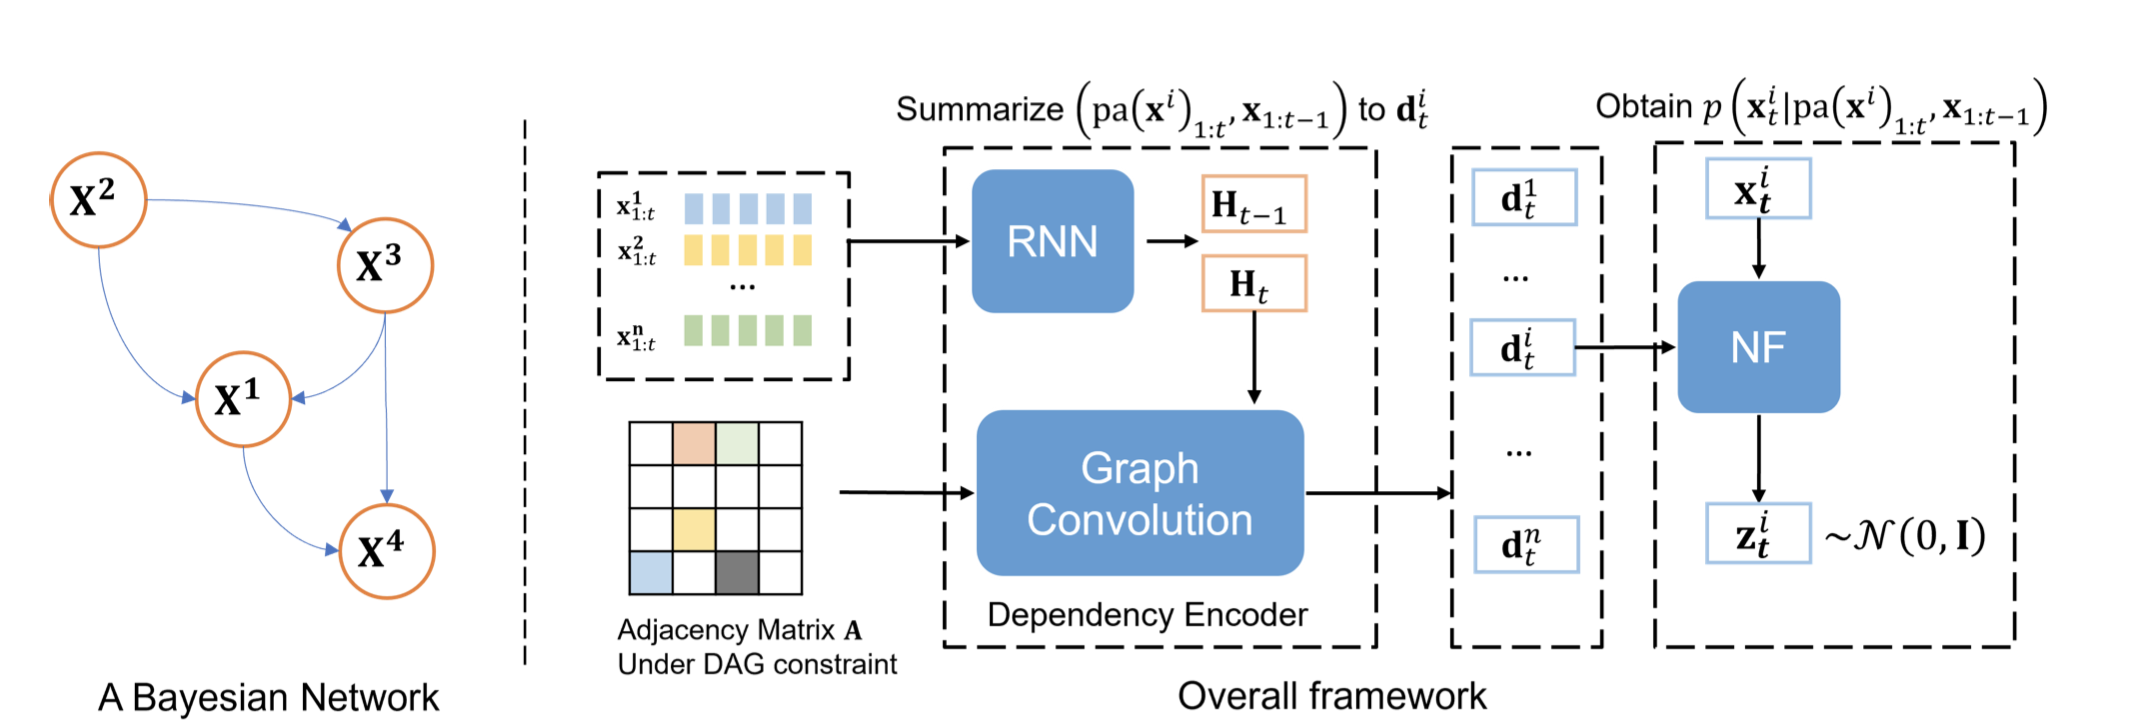
\includegraphics[width = 1\textwidth]{chapter1/GANF.jpg}
    \caption{GANF 模型整体架构\cite{ganf}}
    \end{figure}
如图所示, GANF 使用了一个贝叶斯网络,并通过 RNN 沿着序列维度对$p(\mathcal{X})$ 进行因子分解 然后使用条件规范化流对时间维度进行因子分解。然后,采用一种新的基于图的依赖性编码器来参数化因子分解产生的条件概率。用于因子分解的 DAG 是一个离散的对象,通常很难学习,但是,离散的结构通过一个可微的图形 $\mathbf { a } $反映在依赖编码器中,这个图形的邻接矩阵就是 $\mathbf { a } $。此外,$\mathbf { A } $必须对应于 DAG 的要求可以表示为一个可微方程。因此,可以通过使用基于梯度的优化来联合优化 $\mathbf { A } $和流组件。

% \subsubsection{基于GNN的深度学习方法}
Deng 等人\cite{gdn}于2021年在AAAI会议上发表了GDN模型。GDN采用 GNN 的方法捕捉多个时间序列之间的关联关系,并通过一个全连接层对未来时刻的数据进行预测,以预测值与真实值之间的差异作为异常分数进行异常检测,这种方法更侧重于多元之间序列之间的相关性特征进行建模。
\begin{figure}[ht]
    \centering
    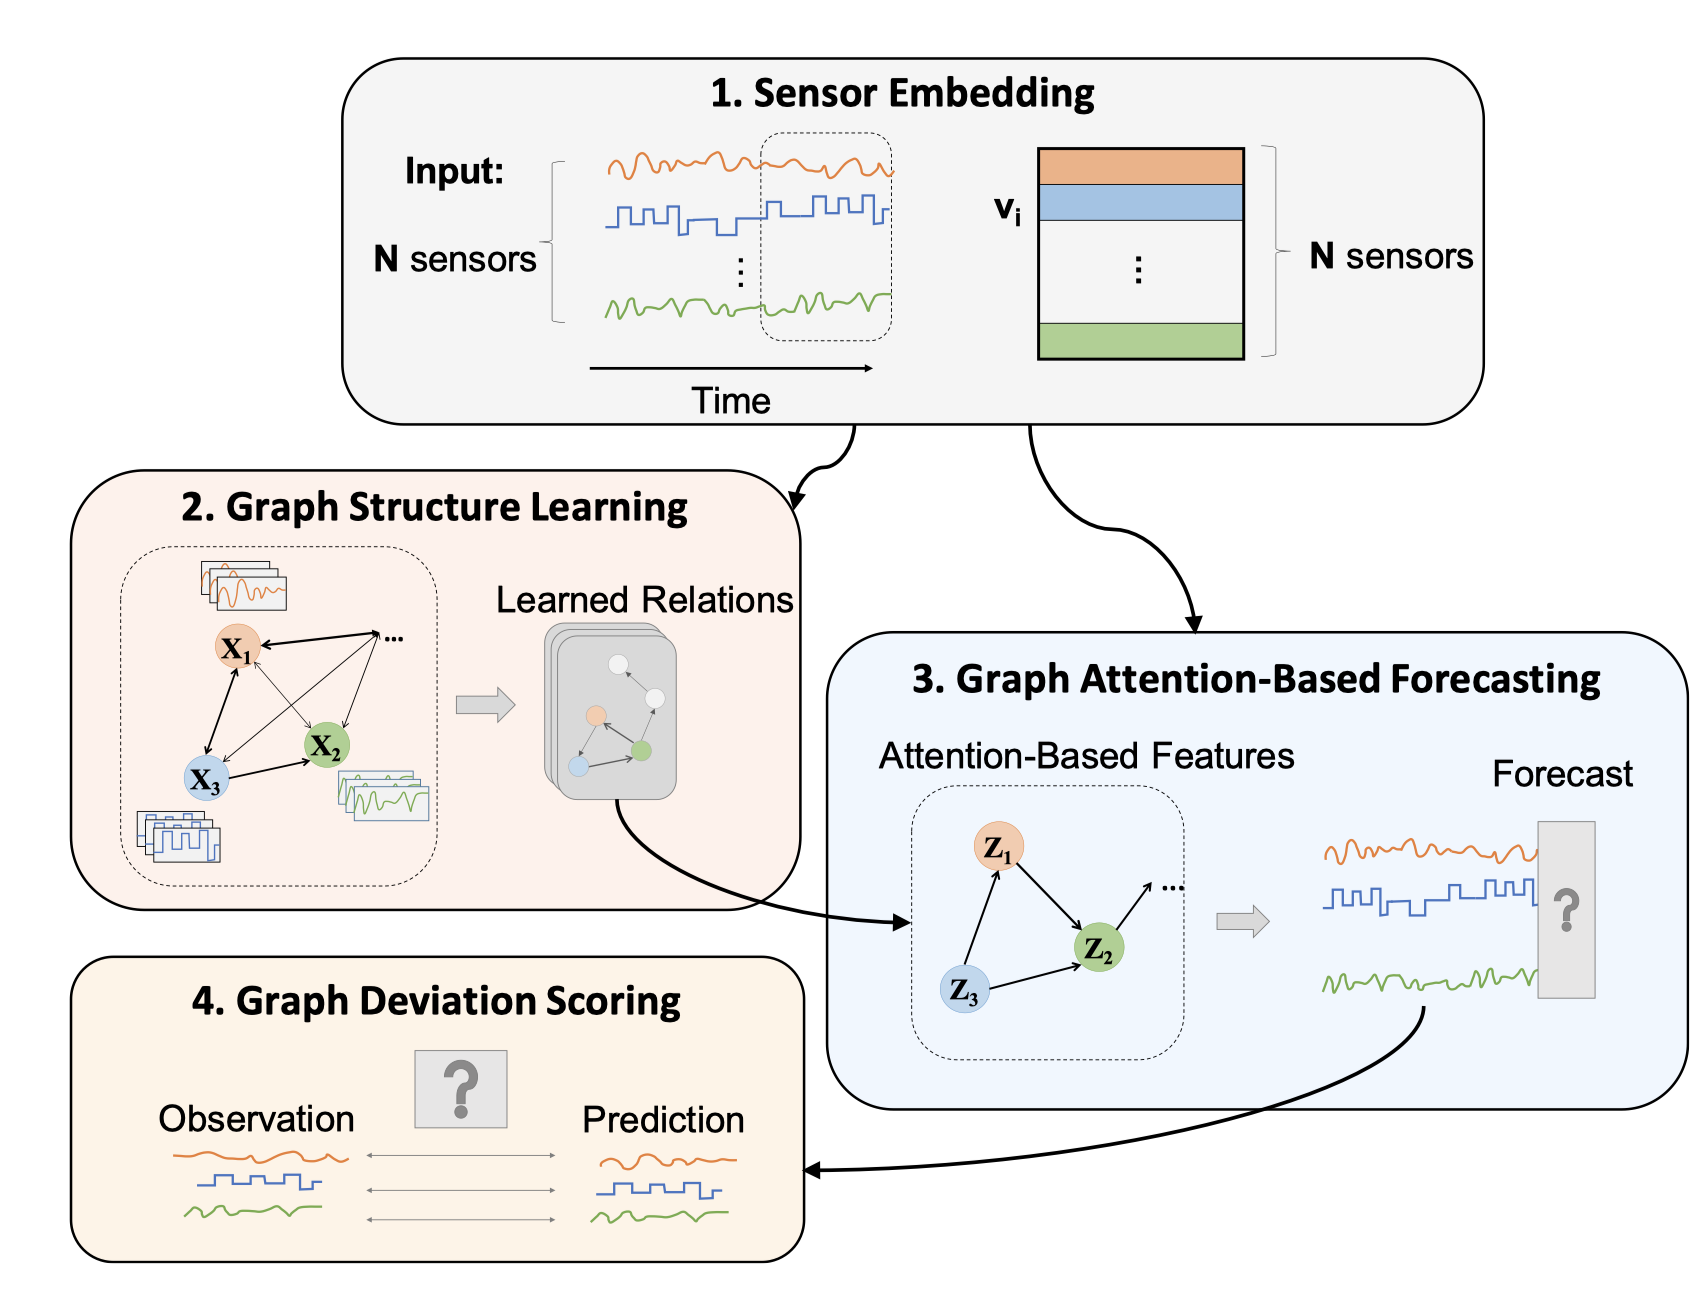
\includegraphics[width = 0.8\textwidth]{chapter1/GDN.jpg}
    \caption{GDN 模型整体架构\cite{gdn}}
    \end{figure}
如图1-2所示,GDN主要包括4个部分,即传感器嵌入, 图结构学习,基于图注意力的预测以及图偏差评分。其中传感器嵌入主要利用嵌入向量捕获每个传感器的独特特性;图结构学习: 学习表示传感器之间依赖关系的图结构;基于图形注意力的预测: 基于图形注意力函数对各传感器的未来值进行预测;图偏差评分: 识别学习关系的偏差,并定位和解释这些偏差。

MTAD-GAT\cite{mtad-gat}使用图形注意网络对特征和时间相关性进行建模,并通过轻量级的门限递归单元(Gated-RecurrentUnit,GRU)网络进行传递,从而在没有严重开销的情况下帮助检测。传统上,注意力操作使用神经网络确定权重的凸组合进行输入压缩。GRU 是 LSTM 的简化版本,参数集较小,可以在有限的数据设置中进行训练。
\begin{figure}[htb]
    \centering
    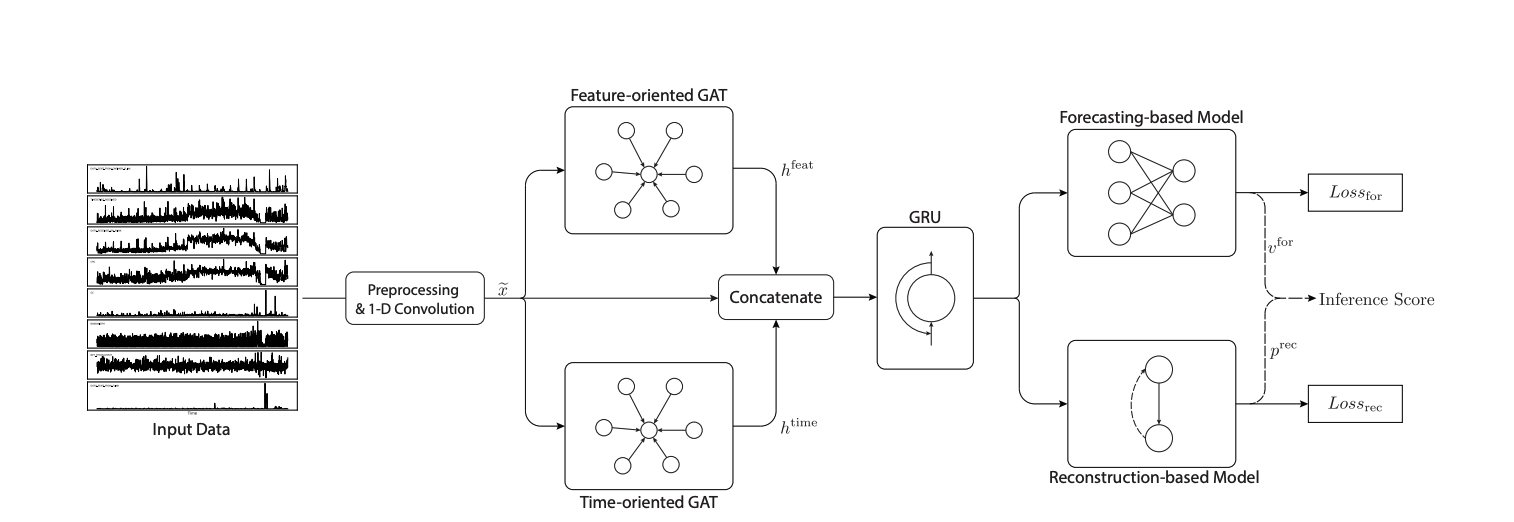
\includegraphics[width = 1\textwidth]{chapter1/MTAD.jpg}
    \caption{MTAD 模型整体架构\cite{mtad-gat}}
    \end{figure}


% \subsubsection{基于GAN的深度学习方法}
Audibert等人\cite{usad}在2020年在KDD上发表了USAD模型。USAD基于自动编码器提出了一种基于对抗性学习的重建方法,该方法通过两个自动编码器对抗性学习重建多元时间序列,并以重建值与真实值之间的差异作为异常分数进行异常检测,这种方法更侧重于对数据的整体分布进行建模。同时Audibert等人提出了训练和检测的两种算法。
\begin{figure}[ht]
    \centering
    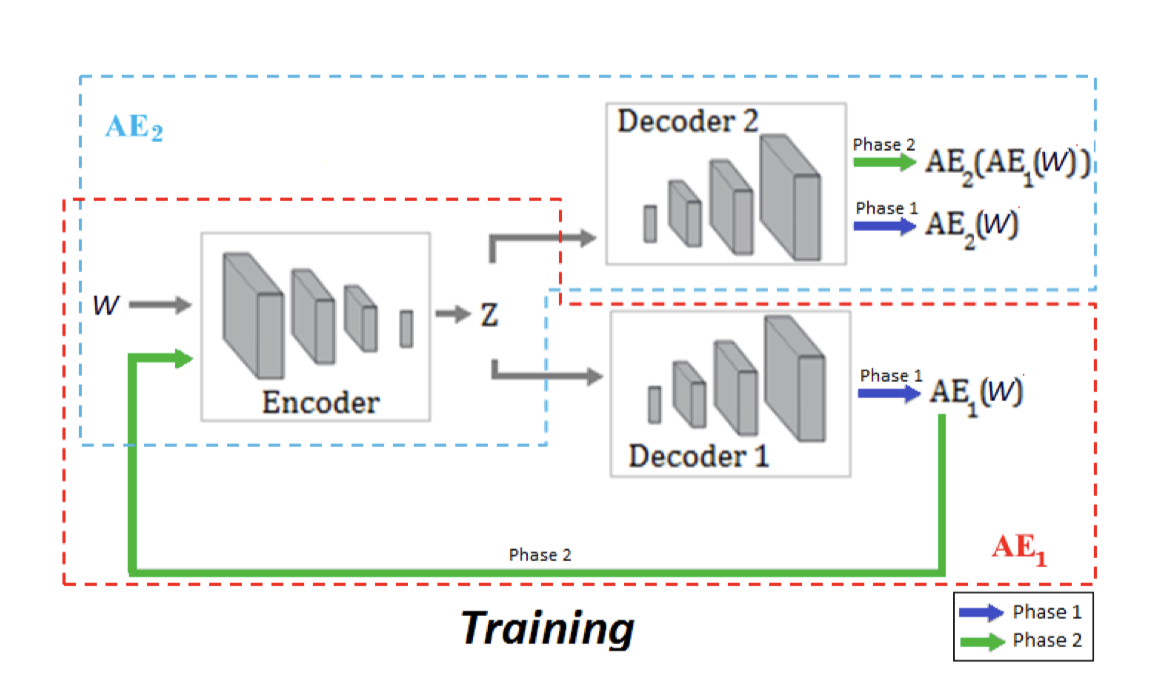
\includegraphics[width = 0.8\textwidth]{chapter1/USAD-TRAINing.jpg}
    \caption{USAD 训练模型架构\cite{usad}}
    \end{figure}
如图1-3所示,USAD模型具有两个自动编码器 AE1和AE2。 在该模型中自动编码器具有双重目的。其中AE1最小化$W$(阶段1)的重建误差,并最小化AE 2(阶段2)的重构输出之间的差异。随着AE1,AE2 最小化了$W$的重建误差(阶段1),它随后最大化了由AE 1(阶段2)重建的输入数据的重建误差。通过这种对抗性学习的方式,使得USAD模型能够更好的学习到时间序列的分布。
\begin{figure}[ht]
    \centering
    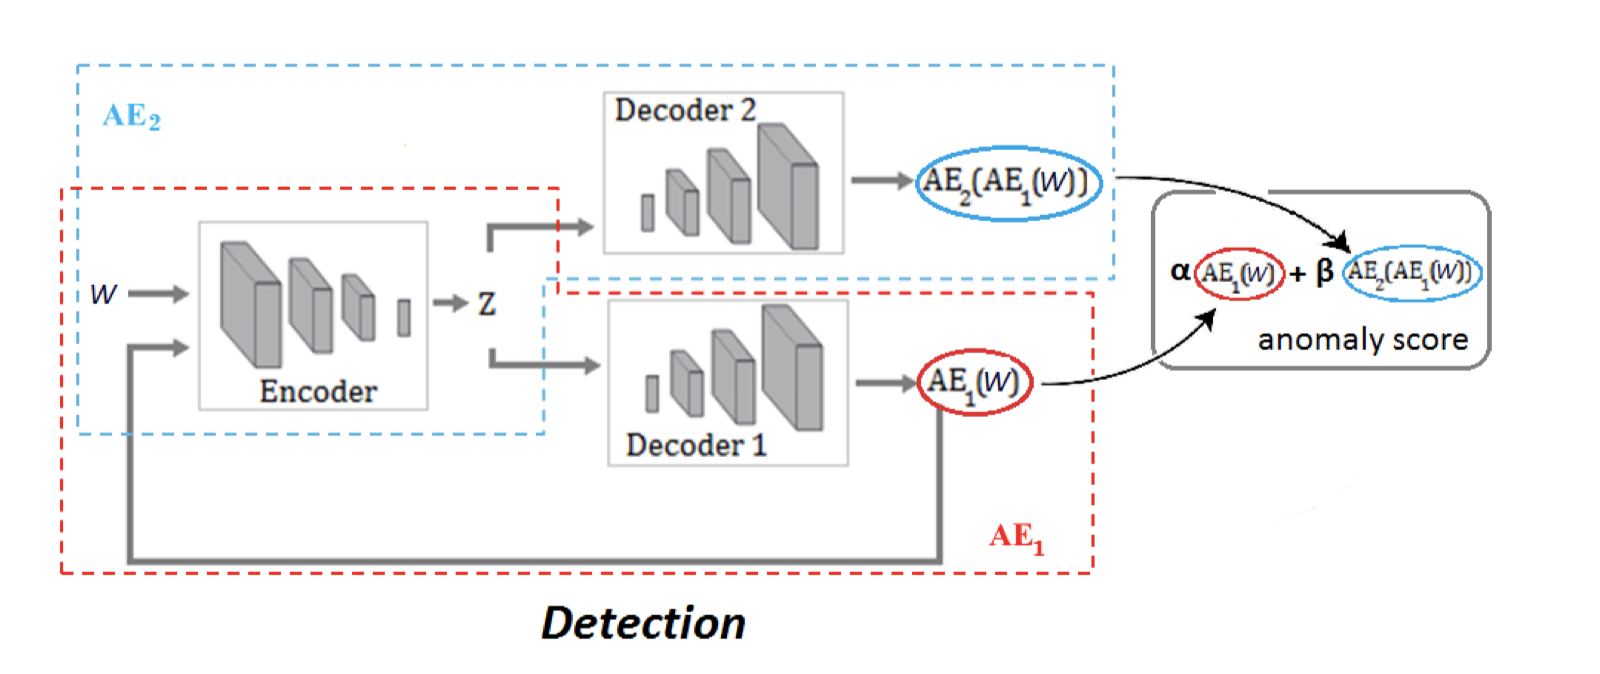
\includegraphics[width = 0.8\textwidth]{chapter1/USAD-DETECTION.jpg}
    \caption{USAD 推断模型架构\cite{usad}}
    \end{figure}
在推断阶段, 时间序列的异常分数通过
\begin{equation}
    \mathscr{A}(\widehat{W})=\alpha\left\|\widehat{W}-A E_1(\widehat{W})\right\|_2+\beta\left\|\widehat{W}-A E_2\left(A E_1(\widehat{W})\right)\right\|_2
    \end{equation}
计算得到,其中$\alpha + \beta = 1$并用于参数化误报和真阳性之间的权衡。如果$\alpha$大于$\beta$,则减少真实阳性的数量并减少误报的数量。相反,如果$\alpha$小于$\beta$,以增加假阳性数量的成本增加了真实阳性的数量。则表示α<βA高检测敏感性方案,而$\alpha > \beta$则表示低检测敏感性。这种参数化方案允许使用单个训练的模型在推断中获得一组不同灵敏度异常得分。

\section{本文的主要研究内容}[Developmental of gas-lubricated bearing]

时间序列异常检测是工业界中一个重要的研究领域。并随着近年来越来越多的行业提倡数字化,智能化,吸引了诸多学者进行研究并提出了非常多的多元时间序列异常检测的算法及模型。然而这些方法都是都是面向完整的时间序列数据进行异常检测任务,然而在真实时间中多元时间序列往往包含着大量的缺失值。例如在工业场景中常常因为数据采集不全,传感器损坏等诸多因素所导致时间序列中包含缺失值。故本文课题为缺失值场景下的多元时间序列异常检测,按照填充-检测和不填充-检测的两种思路对包含缺失值的多元时间序列异常检测任务进行了如下研究:

按照填充-检测的思路,本文首先提出了一种基于对抗生成网络的填充算法,并对填充后的多元时间序列进行异常检测。较好的解决缺失值场景下的多元时间序列异常检测任务。本方法通过与多个基线模型对比,在完整数据集上,本章F1分数超过了第二名的基线0.3\%在缺失30\%数据的场景下F1分数超过了第二名的基线3\%,在缺失50\%数据的场景下F1分数超过了第二名的基线5\%。证明了本文的算法在缺失值场景的有效性。

考虑到在填充-检测的解决方案中,模型在训练时需要同时包含缺失值的时间序列和不包含缺失值的时间序列进行学习。这对数据的要求较高,在现实应用中实现难度较大。填充-检测的思路方案依然不能完美的解决缺失值多元时间序列异常检测问题。故本文提出了一种不填充-检测思路的多元时间序列异常检测方案,其基于注意力机制对缺失值时间序列进行重新表征,将不完整的多元时间序列重新表征为完整的高维表征,进而通过对该表征进行异常检测,更鲁棒的解决缺失值场景下的异常检测任务。本方法在三个常用经典时间序列数据集上进行的实验表明,该方法在缺失值场景下对比传统时间序列异常检测方法效果更好。最后,本文通过消融实验验证了各模块的有效性。

% 本文的主要研究缺失值场景下的多元时间序列异常检测算法,提出了缺失值场景下的多元时间序列异常检测模型 MMAD (Missing Multi Time Series Anomaly Detection),该模型主要结合自注意力机制条件标准化流来完成缺失值场景下的异常检测算法。最后通过在公开数据集上进行实验验证本文提出的有效性。
% \begin{enumerate}
%     \item 缺失值场景下的多元异常检测算法研究
%     提出一种面向缺失值的多元时间序 列的异常检测算法MMAD (Missing Multi Time Series Anomaly Detection),该算法首次提出了一种缺失值场景下的多元时间序列异常检测解决方案。
%     \item 基于掩码注意力机制的缺失值多元时间序列表征算法
%     提出的一种掩码注意力机制模块 (MMAR)将包含缺失值的不完整时间序列数据映射为完整的高维嵌入表征,该表征融合了时间信息、缺失值信息以及观测值信息;
%     \item 基于条件标准化流的标准化分布变换模块(CNF-AD)
%     提出一种基于条件标准化流的标准化分布变换模块(CNF-AD)对该表征进行重建,该模块学习一个可逆变换函数实现一个简单分布(例如高斯分布)与真实分布近似之间的映射,通过该函数与简单分布计算观测值在真实分布中的近似概率,以该概率作为异常分数进行异常检测。
% \end{enumerate}


\section{论文主要结构与安排}[Main research contents of this subject]
本论文的章节划分安排如下: 第一章是绪论,主要介绍本文的研究背景和意义,面临的挑战以及当前主要的两类异常检测算法研究现状, 在绪论最后总结了本文主要的研究内容。

第二章是缺失值时间序列异常检测技术概述。该章节主要介绍时间序列异常检测技术的基本知识,例如时序数据的异常类型,时间序列的基本属性等;同时介绍了本文所利用到的一些关键技术,例如注意力机制和标准化流技术。

第三章按照填充-检测的思路,首先提出了一种基于对抗生成网络的填充算法,并对填充后的多元时间序列进行异常检测。较好的解决缺失值场景下的多元时间序列异常检测任务。随后通过实验证明本文的算法在缺失值场景的有效性。

第四章按照不填充-检测思路,首先提出了一种基于注意力机制对缺失值时间序列进行重新表征,将不完整的多元时间序列重新表征为完整的高维表征,进而通过对该表征进行异常检测的方案,随后在三个常用经典时间序列数据集上进行的实验表明,该方法在缺失值场景下对比传统时间序列异常检测方法效果更好。最后,本文通过消融实验验证了各模块的有效性。
% % !TEX root = ../main.tex

% 中英标题:\chapter{中文标题}[英文标题]
\chapter{缺失值时间序列异常检测技术概述}[Typesetting pictures]

\section{引言}[Introduction]
本章是缺失值时间序列异常检测技术的相关理论基础。首先介绍了什么是时间序列中的异常,即时间序列异常的相关类型,包括点异常,上下文异常,集合异常和其他异常等。然后有关时间序列相关特性,即时间序列的相关属性,包括时序性,维度,非平稳性,噪声等属性。之后介绍了有关注意力机制相关技术,首先介绍了注意力机制的基本原理,然后介绍了注意力机制的计算方式及公式。最后介绍了标准化流的相关技术,包括当前主流实现标准化流的几种方式,即可加性耦合层,仿射耦合层等。

\section{时序数据的异常类型}[Doctoral picture example]
霍金斯\cite{hawkings}将异常值描述为一种与其他观察结果大相径庭的观察结果,以至于引起怀疑,认为它是由另一种机制产生的。在这种情况下,本文将时间序列数据中的异常描述为时间步骤中的数据点,这些数据点显示出与以前的时间步骤显著不同的意外行为。根据以往的文献,本文将与时间序列数据相关的异常分类如下。

点异常是突然偏离标准的数据点或序列。这样的异常似乎是时间噪声,通常是由传感器错误或异常系统操作引起的。为了进行检测,传统上设置了基于先前数据的上下控制限制,通常分别称为 UCL 和 LCL。这些极限之外存在的值被认为是点异常。
\begin{figure}[ht]
    \centering
    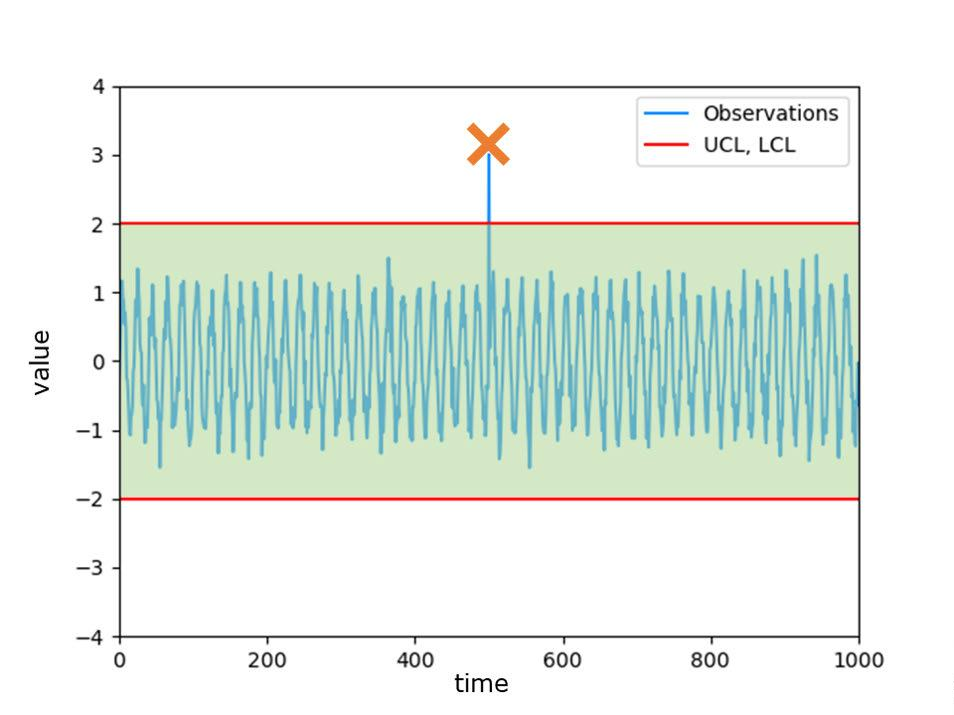
\includegraphics[width = 0.4\textwidth]{chapter2/point-anomaly.png}
    \caption{点异常}
    \end{figure}

与点异常类似,上下文异常表示在短时间内观察到的数据点或序列,但与预定义的 UCL 和 LCL 分界异常相同,不偏离正常范围。然而,考虑到给定的上下文 ,数据点脱离了预期的模式或形状。由于这个原因,这些异常可能很难检测到。
\begin{figure}[ht]
    \centering
    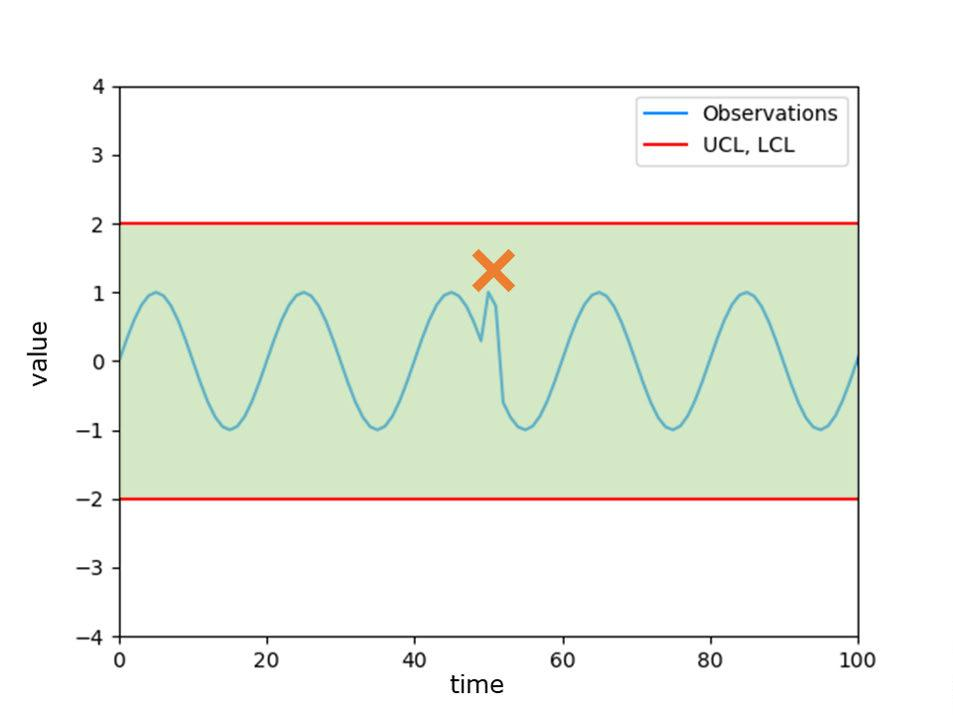
\includegraphics[width = 0.4\textwidth]{chapter2/context.png}
    \caption{上下文异常}
    \end{figure}

这种异常指的是一组数据点,这些数据点应该被视为异常,因为它们随着时间的推移逐渐显示出与正常数据不同的模式。这种异常类型中的个体价值观看起来似乎没有问题,但是作为一个整体,它们引起了怀疑。由于它们不容易一下子识别出来,所以从长远来看,上下文对于识别它们尤为重要。
\begin{figure}[ht]
    \centering
    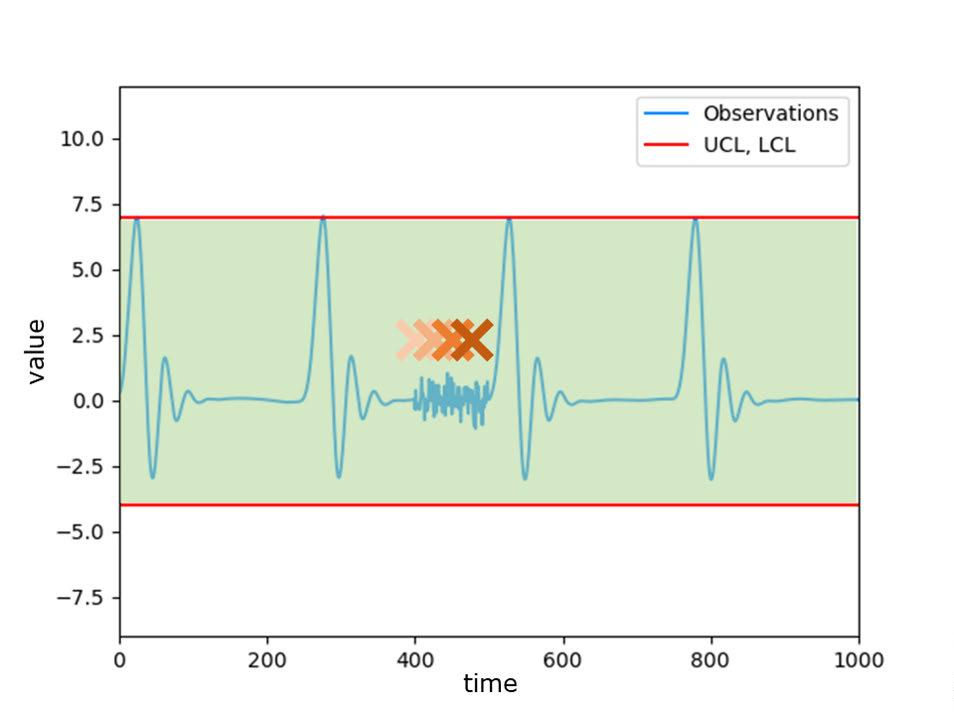
\includegraphics[width = 0.4\textwidth]{chapter2/colletective.png}
    \caption{上下文异常}
    \end{figure}

因为异常是正常状态之外的东西,所以什么是异常取决于对正常的定义。一般来说,异常可以分为上述三种类型之一,但其他观点可以细分为更具体的异常类别。

总之,异常是一种数据点,其发生在过去极为罕见,或者在逻辑上是不可能的。然而,在多变量时间序列数据中,可能不能像前面的例子那样对异常进行分类。多变量时间序列数据需要额外考虑变量与时间轴之间的关系。随着变量数量的增加,出现了更多多样化的模式。然后,异常模式可能是不规则的,并且正常状态和异常状态之间的差异可能是模糊的。扫描单个单变量时间序列数据并将其聚合以识别异常,并不能保证检测结果的准确性,因为很少有异常点会被其他正常变量掩盖,并对整个目标系统产生重大影响。通过提取清晰的变量或特征或使用足够复杂的模型来检测各种模式来减少维度可以解决这些问题。

\begin{figure}[htbp]
    \centering
    \subfigure{
    \begin{minipage}[t]{0.5\linewidth}
    \centering
    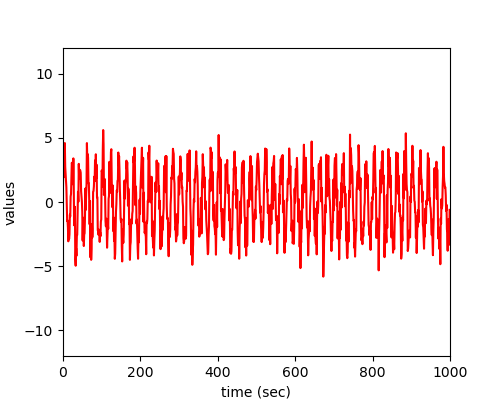
\includegraphics[width=2in]{chapter2/normal-1.png}
    \caption{正常时间序列}
    \end{minipage}%
    }%
    \subfigure{
    \begin{minipage}[t]{0.5\linewidth}
    \centering
    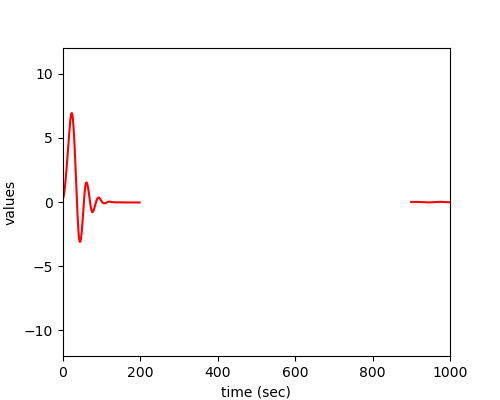
\includegraphics[width=2in]{chapter2/missing-2.png}
    \caption{数据丢失异常}
    \end{minipage}%
    }%
    % \subfigure{
    % \begin{minipage}[t]{0.25\linewidth}
    % \centering
    % 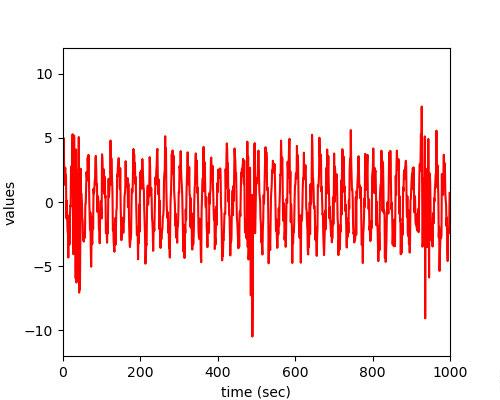
\includegraphics[width=1in]{chapter2/outlier-1.png}
    % \caption{数据点离群异常}
    % \end{minipage}
    % }%
    % \subfigure{
    % \begin{minipage}[t]{0.25\linewidth}
    % \centering
    % 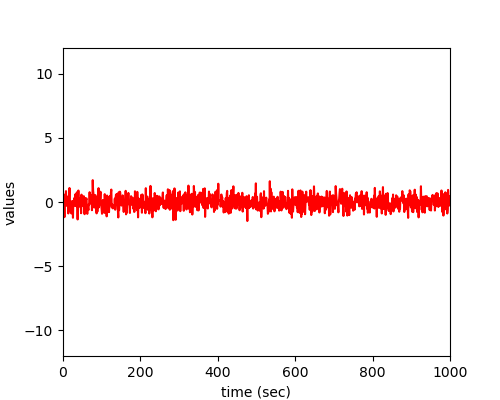
\includegraphics[width=1in]{chapter2/3-1.png}
    % \caption{时间序列频率异常}
    % \end{minipage}
    % }%
    \centering
    %\caption{其他异常举例}
    \end{figure}

\begin{figure}[htbp]
    \centering
    % \subfigure{
    % \begin{minipage}[t]{0.25\linewidth}
    % \centering
    % 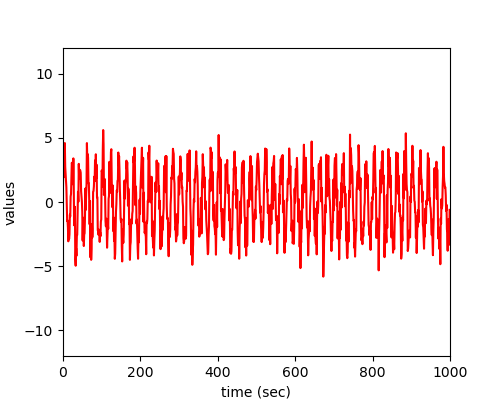
\includegraphics[width=1in]{chapter2/normal-1.png}
    % \caption{正常时间序列}
    % \end{minipage}%
    % }%
    % \subfigure{
    % \begin{minipage}[t]{0.25\linewidth}
    % \centering
    % 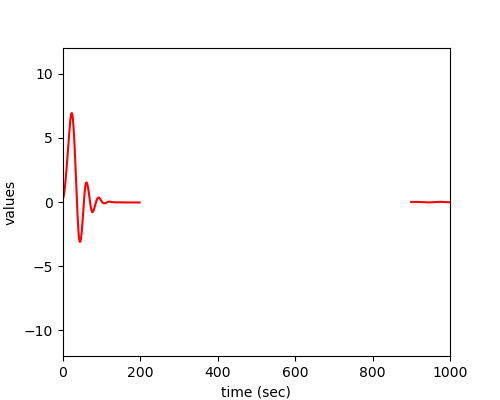
\includegraphics[width=1in]{chapter2/missing-2.png}
    % \caption{数据丢失异常}
    % \end{minipage}%
    % }%
    \subfigure{
    \begin{minipage}[t]{0.5\linewidth}
    \centering
    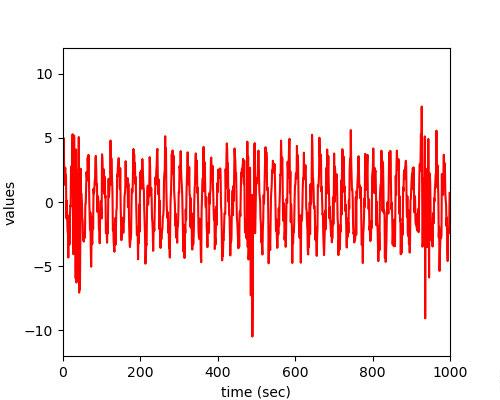
\includegraphics[width=2in]{chapter2/outlier-1.png}
    \caption{数据点离群异常}
    \end{minipage}
    }%
    \subfigure{
    \begin{minipage}[t]{0.5\linewidth}
    \centering
    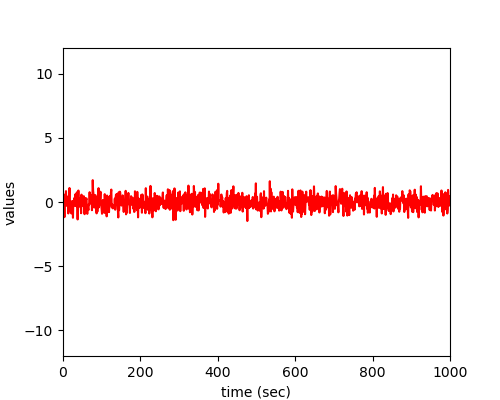
\includegraphics[width=2in]{chapter2/3-1.png}
    \caption{时间序列频率异常}
    \end{minipage}
    }%
    \centering
    %\caption{其他异常举例}
    \end{figure}

\section{时间序列相关属性}
虽然在几乎所有的任务中,时间都是一个基本概念,但处理时间敏感的数据需要仔细考虑。然而,如果很好地理解时间序列数据的特征,则可以通过利用来自信号的上下文信息来有效地检测异常。因此,我们简要描述了时间序列数据的基本原理。这里讨论的因素包括时间性、维数、非平稳性和噪声。

时间序列通常被认为是按时间顺序索引的观测值的集合。数据以相等的间隔捕获,序列中的每个连续数据点取决于其过去的值。因此,每个连续观测值之间存在一定的时间相关性或相关性[19]。观测序列的联合分布可以使用链积规则表示为。
\begin{equation}
	p\left(x^1, x^2, \ldots, x^T\right)=p\left(x^1\right) \prod_{t=2}^T p\left(x^t \mid x^1, x^2, \ldots, x^{t-1}\right)
	\end{equation}
其中 $x^t$ 是在时间 $t \in T \subseteq \mathbb{Z}^{+}$ 时观察到的数据点,每个条件概率 $p(\cdot \mid \cdot)$ 表示当前状态和以前状态之间的时间依赖关系。

维度是指每个观察中捕获的单个数据属性的数量\cite{yellow1}。根据维度,时间序列数据在很大程度上分为单变量和多变量类型。时间序列数据的维度影响计算成本和分析方法。单变量:这种类型描述了一组有序的实值观测值,其中每个数据点在一个特定的时间被测量,$t \in T \subseteq \mathbb{Z}^{+}$ 。然后,$x^t \in \mathbb{R}$ 是在时间 $t$ 处测量的数据点,是某个随机变量 $X^t$ 的实现值。 这种类型描述了一组有序的多维向量,$X=\left\{\mathbf{x}^t\right\}_{t \in T}$,每个向量在特定的时刻被记录,$t \in T \subseteq \mathbb{Z}^{+}$,并且包含实值观测值。在实际情况下,这可以看作是一组单变量时间序列数据流,表示目标系统的状态。

单变量时间序列的异常检测只考虑当前状态和以前状态之间的关系,即时间依赖。但是对于多变量流,时间相关性和观测值之间的相关性都需要考虑。尽管增加了一些技巧,多变量时间序列数据现在已经成为一种典型的数据类型,用于分析由多个变量组合产生的各种行为


如果一个时间序列的统计特性不随时间变化,那么它就是平稳的。更明确地说,对于任意 $\tau \in \mathbb{N}$,如果满足下列条件,连续随机过程 $\mathbf{x}=\left\{x^t\right\}_{t \in T \subset \mathbb{Z}^{+}}$ 是强平稳的,即:
\begin{equation}
    F_{\mathbf{x}}\left(x^{1+\tau}, \ldots, x^{t+\tau}\right)=F_{\mathbf{x}}\left(x^1, \ldots, x^t\right)
    \end{equation}
由于大多数时间序列数据是非平稳的,所以在特定时间戳下表明虚假异常的数据点在更大范围内可能不是真正的异常。因此,适应数据结构变化的检测方法是长期部署所必需的。

在信号处理中,噪声是对信号在捕获、存储、传输、处理或转换过程中发生的不必要变化的通用术语\cite{yellow23}。在现实世界的系统中,它被认为是一个基本问题。在许多情况下,噪音是由于传感器灵敏度的微小波动造成的,基本上不会对整个数据结构产生影响。然而,当噪声系统中噪声和异常之间难以分离时,噪声严重影响检测模型的性能\cite{yellow24}。因此,在预处理阶段,了解噪声的本质和降低噪声是至关重要的。

\section{注意力机制相关技术}

神经网络中的注意力机制(Attention Mechanism)是在计算能力有限的情况下,将计算资源分配给更重要的任务,同时解决信息超载问题的一种资源分配方案。在神经网络学习中,一般而言模型的参数越多则模型的表达能力越强,模型所存储的信息量也越大,但这会带来信息过载的问题。那么通过引入注意力机制,在众多的输入信息中聚焦于对当前任务更为关键的信息,降低对其他信息的关注度,甚至过滤掉无关信息,就可以解决信息过载问题,并提高任务处理的效率和准确性。

这就类似于人类的视觉注意力机制,通过扫描全局图像,获取需要重点关注的目标区域,而后对这一区域投入更多的注意力资源,获取更多与目标有关的细节信息,而忽视其他无关信息。通过这种机制可以利用有限的注意力资源从大量信息中快速筛选出高价值的信息。

在神经网络模型处理大量输入信息的过程中,利用注意力机制,可以做到只选择一些关键的的输入信息进行处理,来提高神经网络的效率,比如在机器阅读理解任务中,给定一篇很长的文章,然后就文章的内容进行提问。提出的问题只和段落中一两个句子有关,其余部分都是无关的,那么只需要把相关的片段挑出来让神经网络进行处理,而不需要把所有文章内容都输入到神经网络中。

用数学语言来表达这个思想就是:用$X=[x_1, x_2, ..., x_N]$表示N个输入信息,为了节省计算资源,不需要让神经网络处理这N个输入信息,而只需要从X中选择一些与任务相关的信息输进行计算。软性注意力(Soft Attention)机制是指在选择信息的时候,不是从N个信息中只选择1个,而是计算N个输入信息的加权平均,再输入到神经网络中计算。相对的,硬性注意力(Hard Attention)就是指选择输入序列某一个位置上的信息,比如随机选择一个信息或者选择概率最高的信息。但一般还是用软性注意力机制来处理神经网络的问题。

注意力值的计算可以分为两步:在所有输入信息上计算注意力分布,根据注意力分布来计算输入信息的加权平均。

给定这样一个场景:把输入信息向量X看做是一个信息存储器,现在给定一个查询向量q,用来查找并选择X中的某些信息,那么就需要知道被选择信息的索引位置。采取“软性”选择机制,不是从存储的多个信息中只挑出一条信息来,而是雨露均沾,从所有的信息中都抽取一些,只不过最相关的信息抽取得就多一些。

于是定义一个注意力变量$z\in [1, N]$来表示被选择信息的索引位置,即$z=i$来表示选择了第i个输入信息,然后计算在给定了q和X的情况下,选择第i个输入信息的概率$\alpha _i$

\begin{equation}
    \begin{aligned}
    \alpha_i &=p(z=i \mid X, \mathbf{q}) \\
    &=\operatorname{softmax}\left(s\left(\mathbf{x}_i, \mathbf{q}\right)\right) \\
    &=\frac{\exp \left(s\left(\mathbf{x}_i, \mathbf{q}\right)\right)}{\sum_{j=1}^N \exp \left(s\left(\mathbf{x}_j, \mathbf{q}\right)\right)}
    \end{aligned}
    \end{equation}

其中$\alpha _i$构成的概率向量就称为注意力分布(Attention Distribution)。$s(x_i , q)$是注意力打分函数。当前注意力打分函数主要有4类,加性模型, 点积模型,缩放点积模型,双线性模型;其公式主要如下列所示:
\begin{equation}
    \quad s\left(\mathbf{x}_i, \mathbf{q}\right)=\mathbf{v}^{\mathrm{T}} \tanh \left(W \mathbf{x}_i+U \mathbf{q}\right)
\end{equation}
\begin{equation}
    \quad s\left(\mathbf{x}_i, \mathbf{q}\right)=\mathbf{x}_i^{\mathrm{T}} \mathbf{q}    
\end{equation}
\begin{equation}
    \quad s\left(\mathbf{x}_i, \mathbf{q}\right)=\frac{\mathbf{x}_i^{\mathrm{T}} \mathbf{q}}{\sqrt{d}}    
\end{equation}
\begin{equation}
    s\left(\mathbf{x}_i, \mathbf{q}\right)=\mathbf{x}_i^{\mathrm{T}} W \mathbf{q}
\end{equation}

其中$W$、$U$和$v$是可学习的网络参数,$d$是输入信息的维度。

注意力分布$\alpha _i$表示在给定查询$q$时,输入信息向量$X$中第$i$个信息与查询q的相关程度。采用“软性”信息选择机制给出查询所得的结果,就是用加权平均的方式对输入信息进行汇总,得到Attention值:
\begin{equation}
    \operatorname{att}(X, \mathbf{q})=\sum_{i=1}^N \alpha_i \mathbf{x}_i
    \end{equation}

下图是计算Attention值的过程图:
\begin{figure}[ht]
    \centering
    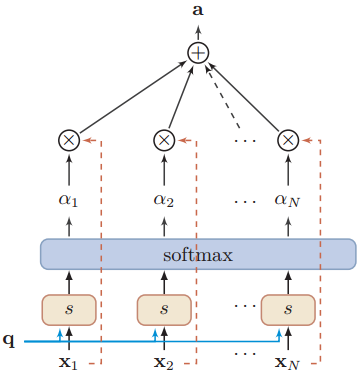
\includegraphics[width = 0.4\textwidth]{chapter2/attension.png}
    \caption{计算Attension值的过程图}
    \end{figure}

更一般的,可以用键值对(key-value pair)来表示输入信息,那么$N$个输入信息就可以表示为

\begin{equation}
	\begin{aligned}	
    (K, V)= [(k_1,v_1),(k_2,v_2),\ddots,(k_N,v_N)](K, V) \\
    &= [(k_1,v_1),(k_2,v_2),\ddots,(k_N,v_N)]
	\end{aligned}
\end{equation}

其中“键”用来计算注意分布$\alpha _i$,“值”用来计算聚合信息。
那么就可以将注意力机制看做是一种软寻址操作:把输入信息X看做是存储器中存储的内容,元素由地址Key(键)和值Value组成,当前有个Key=Query的查询,目标是取出存储器中对应的Value值,即Attention值。而在软寻址中,并非需要硬性满足Key=Query的条件来取出存储信息,而是通过计算Query与存储器内元素的地址Key的相似度来决定,从对应的元素Value中取出多少内容。每个地址Key对应的Value值都会被抽取内容出来,然后求和,这就相当于由Query与Key的相似性来计算每个Value值的权重,然后对Value值进行加权求和。加权求和得到最终的Value值,也就是Attention值。

以上的计算可以归纳为三个过程:根据Query和Key计算二者的相似度。可以用上面所列出的加性模型、点积模型或余弦相似度来计算,得到注意力得分$s_i$;
\begin{equation}
    s_i=F\left(Q, k_i\right)
    \end{equation}
用softmax函数对注意力得分进行数值转换。一方面可以进行归一化,得到所有权重系数之和为1的概率分布,另一方面可以用softmax函数的特性突出重要元素的权重;
\begin{equation}
    \alpha_i=\operatorname{softmax}\left(s_i\right)=\frac{\exp \left(s_i\right)}{\sum_{j=1}^N \exp \left(s_j\right)}
    \end{equation}
根据权重系数对Value进行加权求和:
\begin{equation}
    \operatorname{Attention}((K, V), Q)=\sum_{i=1}^N \alpha_i v_i
    \end{equation}

\begin{figure}[ht]
    \centering
    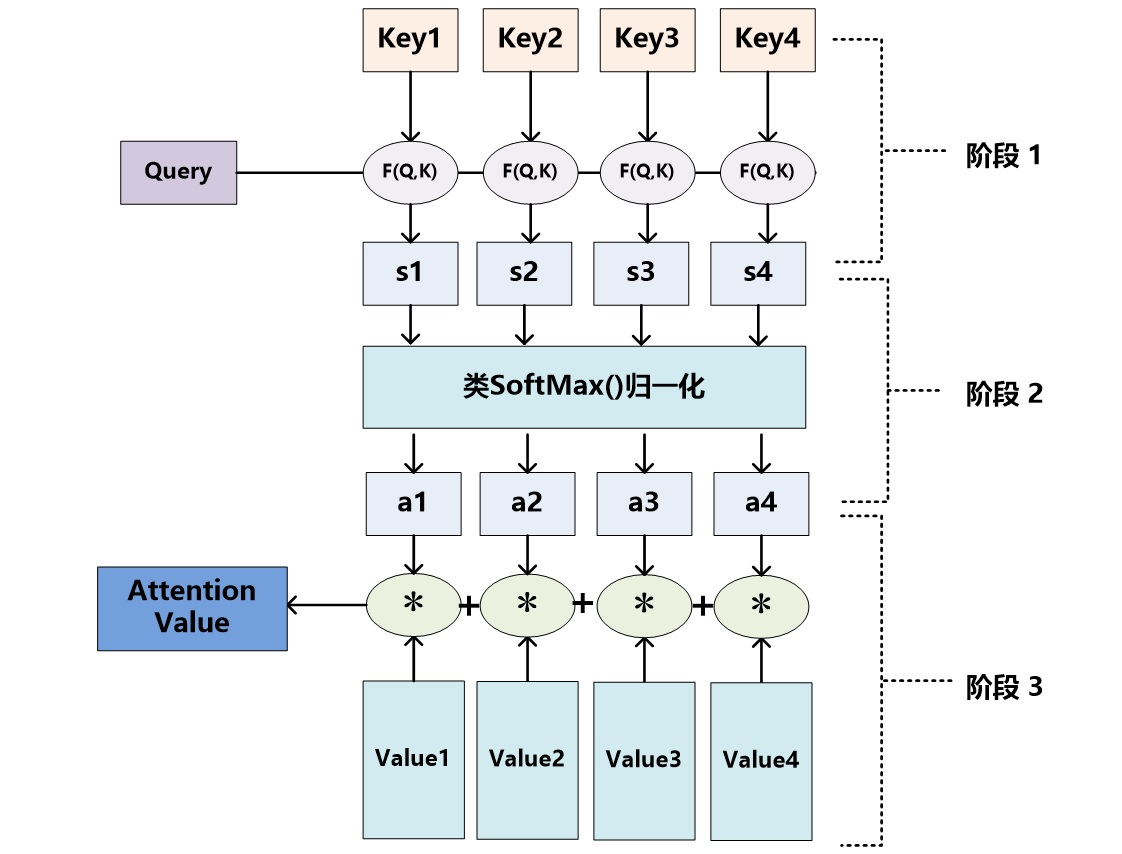
\includegraphics[width = 0.8\textwidth]{chapter2/attesion2.png}
    \caption{键值对注意力模式}
    \end{figure}
故可以得到整体注意力计算公式:
\begin{equation}
    \begin{aligned}
    \operatorname{att}((K, V), \mathbf{q}) &=\sum_{i=1}^N \alpha_i \mathbf{v}_i \\
    &=\sum_{i=1}^N \frac{\exp \left(s\left(\mathbf{k}_i, \mathbf{q}\right)\right)}{\sum_j \exp \left(s\left(\mathbf{k}_j, \mathbf{q}\right)\right)} \mathbf{v}_i
    \end{aligned}
    \end{equation}

%csdn https://blog.csdn.net/qq_37492509/article/details/114991482


\section{标准化流相关技术}
多年来,研究人员发明了许多方法来学习大型数据集的概率分布,包括生成对抗网络(GAN)\cite{gan}、变分自编码器(VAE)\cite{vae}和标准化流\cite{nf}等。GAN和VAE的能力本已十分惊人,它们都能通过简单的推理方法学习十分复杂的数据分布。然而,GAN和VAE都缺乏对概率分布的精确评估和推理,这往往导致VAE中的模糊结果质量不高,GAN训练也面临着如模式崩溃和后置崩溃等挑战。因此,Normalizing Flow应运而生,试图通过使用可逆函数来解决目前GAN和VAE存在的许多问题。

%原理
标准化流的核心思想是利用分布变换的可逆性 如果 $y=f(x)$, 且 $f$ 是可逆的, 则
\begin{equation}
    \begin{aligned}
        &p_x(x)=p_y(f(x)) *|\operatorname{det} J f(x)| \\
        &p_y(y)=p_x\left(f^{-1}(y)\right) *\left|\operatorname{det} J f^{-1}(y)\right|
        \end{aligned}
\end{equation}

当存在多个 $f$ 复合时, 可以在取log之后求和:
\begin{equation}
    \begin{aligned}
    \mathbf{z}_K &=f_K \circ \ldots \circ f_2 \circ f_1\left(\mathbf{z}_0\right) \\
    \log q_K\left(\mathbf{z}_K\right) &=\log q_0\left(\mathbf{z}_0\right)-\sum_{k=1}^K \log \operatorname{det}\left|\frac{\partial f_k}{\partial \mathbf{z}_k}\right|
    \end{aligned}
    \end{equation}

当前基于标准化流主要有三种实现方式,即,可加性耦合层\cite{nice},仿射耦合层\cite{realnvp},可逆的1x1卷积\cite{glow},其中可加性耦合层的做法:首先对于D维数据的 $x$, 将其随意地划分为两部分, $x_1, x_2$ ,并做变换:
\begin{equation}
    \begin{aligned}
        &\mathbf{y}_1=\boldsymbol{x}_1 \\
        &\mathbf{y}_2=\boldsymbol{x}_2+\boldsymbol{m}\left(\boldsymbol{x}_1\right)
        \end{aligned}
\end{equation}
其中m是一个任意的MLP函数, 通过这样的变换, 如果这个函数是可逆的, 即:
\begin{equation}
    \begin{aligned}
        &x_1=\mathbf{y}_1 \\
        &x_2=\mathbf{y}_2-\boldsymbol{m}\left(\boldsymbol{x}_1\right)
        \end{aligned}
\end{equation}

仿射耦合层提出了一种相对可加性耦合层复杂一点的方法, 即
\begin{equation}
    \begin{aligned}
        &\mathbf{y}_1=\boldsymbol{x}_1 \\
        &\mathbf{y}_2=\mathbf{s}\left(\mathbf{x}_1\right) \odot \boldsymbol{x}_2+t\left(\boldsymbol{x}_1\right)
        \end{aligned}
\end{equation}

通过乘一个非线性函数 $\mathbf{s}\left(\mathbf{x}_1\right)$, 本质上是一个线性变换。此处仿射耦合层的雅可比矩阵为:
\begin{equation}
    \frac{\partial \mathbf{y}}{\partial \mathbf{x}}=\left[\begin{array}{ll}
        \frac{\partial y_1}{\partial x_1} & \frac{\partial y_1}{\partial x_2} \\
        \frac{\partial y_2}{\partial x_1} & \frac{\partial y_2}{\partial x_2}
        \end{array}\right]=\left[\begin{array}{cc}
        \mathbb{I}_d & 0 \\
        \frac{\partial \mathbf{s}}{\partial \mathbf{x}_1} \otimes \mathbf{x}_2+\frac{\partial t}{\partial \mathbf{x}_1} & \operatorname{diag}(s)
        \end{array}\right]
\end{equation}

因为
\begin{equation}
    \left(\begin{array}{c}
        x_1 \\
        \vdots \\
        x_n
        \end{array}\right) \odot\left(\begin{array}{c}
        y_1 \\
        \vdots \\
        y_n
        \end{array}\right)=\left(\begin{array}{ccc}
        x_1 & \cdots & 0 \\
        \vdots & \ddots & \vdots \\
        0 & \cdots & x_n
        \end{array}\right)\left(\begin{array}{c}
        y_1 \\
        \vdots \\
        y_n
        \end{array}\right)
\end{equation}
所以在这里雅可比矩阵也是一个对角矩阵, 即$\frac{\partial y_2}{\partial x_2}=\frac{\partial \operatorname{diag}(\mathbf{s}) x_2}{\partial x_2}=\operatorname{diag}(\mathbf{s})$。

可逆的1x1卷积做法是将一个卷积核表达成一个矩阵乘积, 即可以写出一个矩阵的计算公式:$Y=XW$
比如, $x$ 是 $h * w * c$ 的张量, $\mathrm{c}$ 表示channel, 对于1x1卷积来说, W就是一个 $c * c$ 的矩阵, 就是他们的乘积, 实际上可以将x当成 $h * w$ 行 $c$ 列的矩阵, 乘以W。
利用LU分解,构造一个一定可逆的矩阵 $W$。因为任意矩阵都可以表达成$W=PLU$

其中P是置换矩阵, $\mathrm{L}$ 是下三角矩阵, 对角线元素全为 $1, \mathrm{U}$ 是上三角矩阵, 为了保证矩阵 $W$ 可逆, 需要保证 $P , L$, U满秩, 又因为 $P$, L一定是满秩的, 所以只要保证 $U$ 满秩即可。那么 一个方便的方法就是:
\begin{equation}
    W=P L(U+\operatorname{diag}(s))
\end{equation}
其中, U是严格上三角矩阵, 其对角线为 0, 最终可逆卷积核其导数行列式的求解为:
\begin{equation}
    \begin{aligned}
        &\log \left|\operatorname{det}\left(\frac{d \operatorname{conv} 2 \mathrm{D}(\mathbf{h} ; \mathbf{W})}{d \mathbf{h}}\right)\right|=h \cdot w \cdot \log |\operatorname{det}(\mathbf{W})| \\
        &=h \cdot w \cdot \log |\operatorname{diag}(s)|=h \cdot w \cdot \operatorname{sum}(\log (|s|))
        \end{aligned}
\end{equation}

\section{本章小结}
本章是缺失值时间序列异常检测技术的相关理论基础。首先介绍了什么是时间序列中的异常,即时间序列异常的相关类型,包括点异常,上下文异常,集合异常和其他异常等。然后有关时间序列相关特性,即时间序列的相关属性,包括时序性,维度,非平稳性,噪声等属性。之后介绍了有关注意力机制相关技术,首先介绍了注意力机制的基本原理,然后介绍了注意力机制的计算方式及公式。最后介绍了标准化流的相关技术,包括当前主流实现标准化流的几种方式,即可加性耦合层,仿射耦合层等。
% % !TEX root = ../main.tex

\chapter{基于对抗生成网络的时间序列插值异常检测}[Cite reference]

\section{引言}[Introduction]

多变量时间序列通常含有大量的缺失值,这阻碍了高级分析方法在多变量时间序列数据中的应用。
解决缺失值的挑战的传统方法,包括均值/零插补,案例删除和基于矩阵分解的插补,都不能对多变量时间序列中的时间依赖性和复杂分布的性质进行建模。
本文将缺失值填补问题作为数据生成问题来处理。
受生成对抗网络(GAN)在图像生成方面的成功启发,本章提出用 GAN 学习多变量时间序列数据集的总体分布,进一步用于生成每个样本的缺失值。
与图像数据不同,时间序列数据由于其记录过程的性质,往往是不完整的。
GIAD 采用改进的门回归单元对不完全时间序列的时间不规则性进行建模。
在两个多变量时间序列数据集上的实验表明,该模型在缺失值场景下异常检测精度方面优于基线。

本章的组织结构如下:
3.2 节介绍融合句法信息和情感信息的文本讽刺检 测方法的总体框架以及设计细节;
3.3 节介绍本章实验部分所使用的时间序列据集以及实验设置与结果分析等;
3.4 为本章小结。

\section{基于对抗生成网络的时间序列插值异常检测}
\begin{figure}[ht]
    \label{first-model-overview}
    \centering
    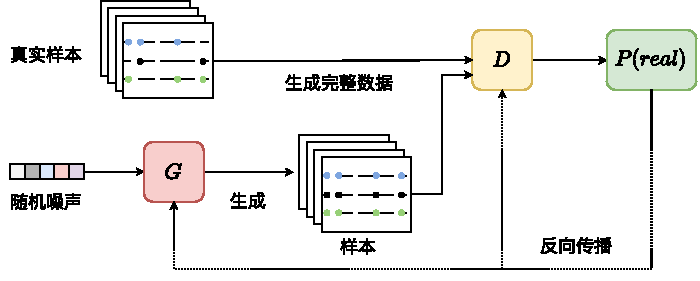
\includegraphics[width = 1\textwidth]{chapter5/overview.pdf}
    \caption{本章模型总体架构图}
    \end{figure}
图~\ref{first-model-overviw}~展示了本章方法的总体架构, 其主要包括以下几个部分: 

\textbf{面向缺失值时间序列的插值门控单元模块}:考虑到缺失值时间序列数据集存在“none”值的存在,两个连续有效观测值之间的时滞总是不断变化的。GRUI模块
通过对传统的GRU模块进行修改,引入了两个连续有效观测值的时滞变量,以保证过去观测结果的影响随着时间而衰减。

\textbf{生成器模块}:生成器模块输入一个随机噪声向量来生成一个假样本,在训练过程中通过损失函数训练生成生成的假样本接近真实样本。

\textbf{判别器模块}:判别器模块输入真实样本与生成器生成的假样本,以真假样本的差异作为损失对模型进行训练。

具体来讲,给定一组具有 $d$ 维的多变量时间序列,在 $\boldsymbol{T}=\left(t_0, \ldots, t_{n-1}\right)$中观察到的一个时间序列  $\boldsymbol{X}$ 表示为 ${X}=\left(\boldsymbol{x}_{t_0}, \ldots, \boldsymbol{x}_{t_i}, \ldots, \boldsymbol{x}_{t_{n-1}}\right)^{\top} \in \mathbb{R}^{n \times d}$, 其中 $x_{t_i}^j$  是 $\boldsymbol{x}_{t_i}$的第 $t_i$ 次观察, $x_{t_i}^j$是 $\boldsymbol{x}_{t_i}$ 的第 $j$  变量。在下面的示例中,$d=4, n=3$和 “None”缺少值。
\begin{equation}
    \boldsymbol{X}=\left[\begin{array}{cccc}
    1 & 6 & \text { none } & 9 \\
    7 & \text { none } & 7 & \text { none } \\
    9 & \text { none } & \text { none } & 79
    \end{array}\right], T=\left[\begin{array}{c}
    0 \\
    5 \\
    13
    \end{array}\right]
    \end{equation}
% The time series $\boldsymbol{X}$ is incomplete, we introduce the mask matrix $\boldsymbol{M} \in \mathbb{R}^{n \times d}$ to present whether the values of $\boldsymbol{X}$ exist or not, i.e., $M_{t_i}^j=1$, if $x_{t_i}^j$ exists, otherwise $M_{t_i}^j=0$.
时间序列 $\boldsymbol{X}$  是不完全的,本章引入掩模矩阵 $\boldsymbol{M} \in \mathbb{R}^{n \times d}$ 来表示 $\boldsymbol{X}$  的值是否存在,即,如果 $M_{t_i}^j=1$, 则$x_{t_i}^j$存在,否则 $M_{t_i}^j=0$。

为了将时间序列数据中缺失的值替换为合理的值,首先训练一个基于 GAN 的模型来学习原始时间序列数据集的分布。在这个自定义 GAN 模型中,从随机输入向量生成假时间序列的生成器和区分假数据和真数据的鉴别器将达到均衡,不仅增加了生成器的代表性能力,而且提高了鉴别器的识别能力(见图3)。其次,确定网络结构,优化生成器的输入随机向量,使生成的假时间序列能够最好地替换缺失值。

\subsection{面向缺失值时间序列的插值门控单元模块}
\begin{figure}[ht]
    \centering
    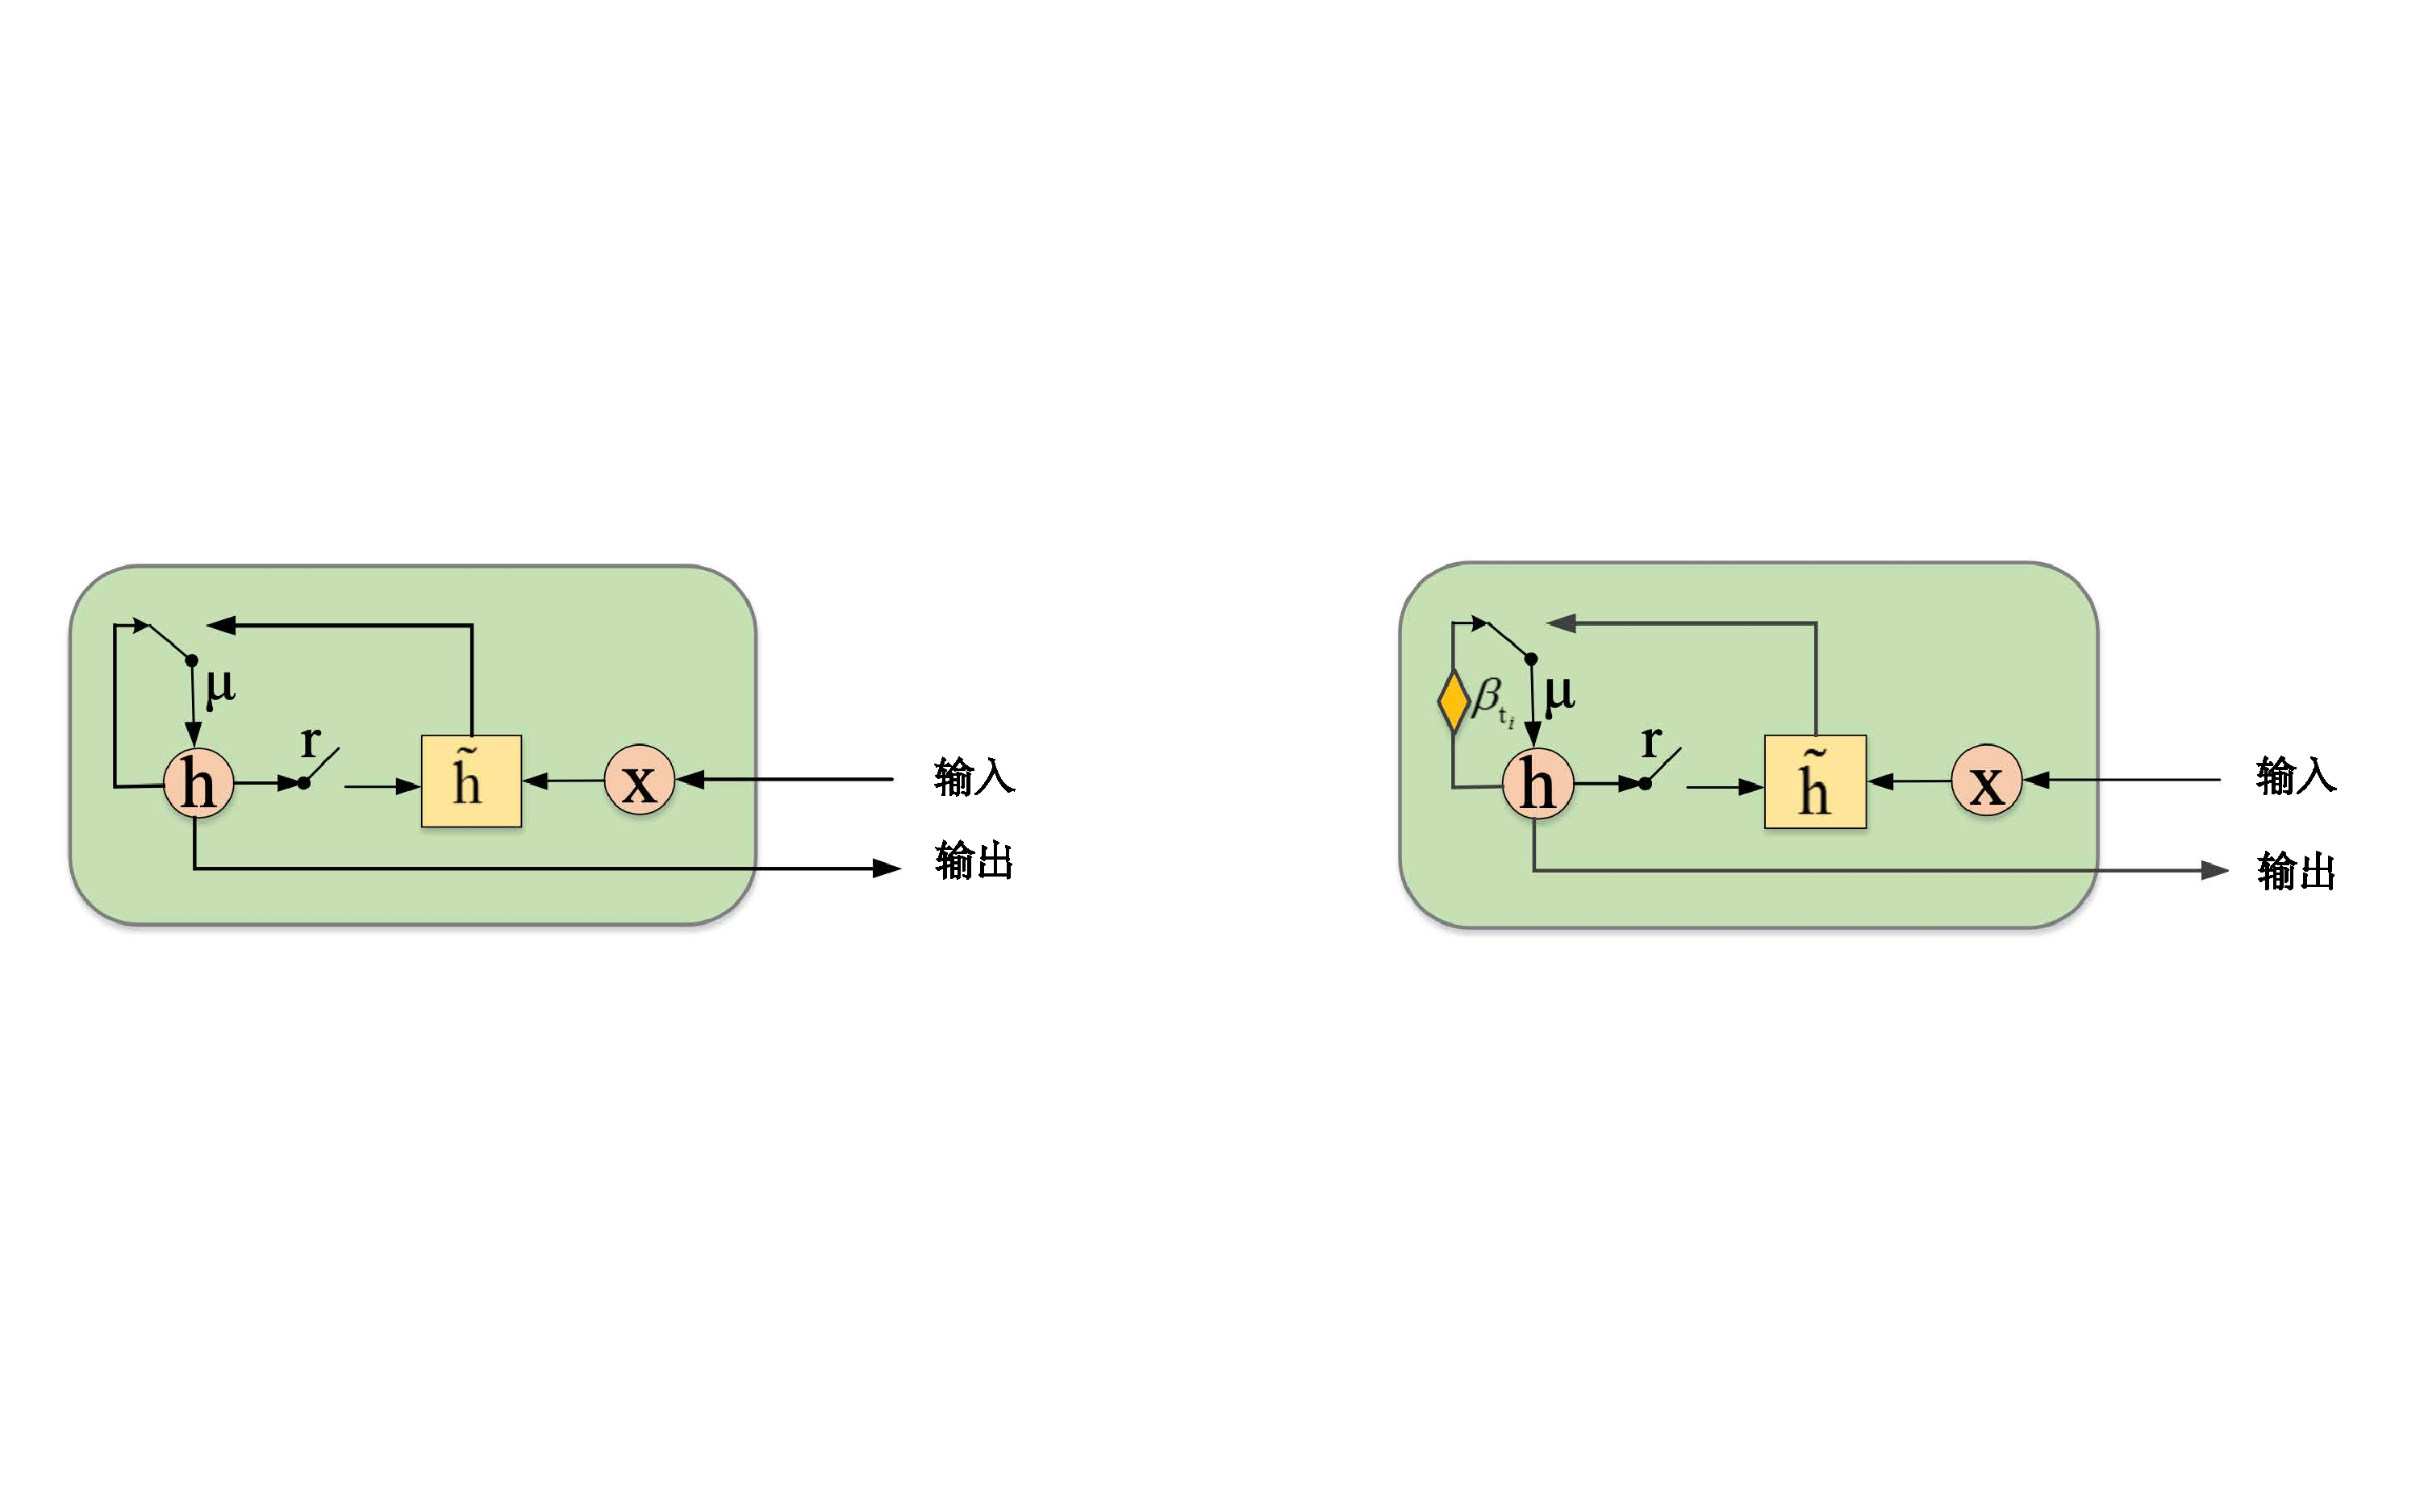
\includegraphics[width = 1\textwidth]{chapter5/GRUI.pdf}
    \caption{本章模型总体架构图}
    \end{figure}
为了适当地了解原始不完全时间序列数据集的分布和特征,并且由于“None”值的存在,两个连续有效观测值之间的时滞总是不断变化的。观测值之间的时滞非常重要,因为它们遵循未知的非均匀分布。这些可变的时间滞后提醒我们,如果变量已经丢失了一段时间,那么过去的观测结果的影响应该随着时间而衰减。为了适应这种衰减的影响,本章提出了门控递归单元的数据插补(GRUI)细胞模型的不完全时间序列的时间不规则性。

% In order to record the time lag of two adjacent existent values of $\boldsymbol{X}$, we introduce the time lag matrix $\boldsymbol{\delta} \in \mathbb{R}^{n \times d}$ to record the time lag between current value and last valid value. The followings is the calculation way and calculated results of $\delta$ of the sample dataset.
为了记录 $\boldsymbol{X}$ 的两个相邻存在值的时滞,引入时滞矩阵$\boldsymbol{\delta} \in \mathbb{R}^{n \times d}$ 来记录当前值与最后一个有效值之间的时滞。下面是样本数据集 $\delta$ 的计算方法和计算结果。
\begin{equation}
    \delta_{t_i}^j=\left\{\begin{array}{ll}
    t_i-t_{i-1}, & M_{t_{i-1}}^j==1 \\
    \delta_{t_{i-1}}^j+t_i-t_{i-1}, & M_{t_{i-1}}^j==0 \& i>0 \\
    0, & i==0
    \end{array} \quad ; \quad \boldsymbol{\delta}=\left[\begin{array}{cccc}
    0 & 0 & 0 & 0 \\
    5 & 5 & 5 & 5 \\
    8 & 13 & 8 & 13
    \end{array}\right]\right.
    \end{equation}
% We introduce a time decay vector $\boldsymbol{\beta}$ to control the influence of the past observations. Each value of the $\boldsymbol{\beta}$ should be bigger than zero and smaller than one, and the larger the $\boldsymbol{\delta}$, the smaller the decay vector.
% So we model the time decay vector $\boldsymbol{\beta}$ as a combination of $\boldsymbol{\delta}$ :
本模型引入一个时间衰减向量 $\boldsymbol{\beta}$ 来控制过去观测的影响。$\boldsymbol{\beta}$ 的每个值应大于0,小于1,$\boldsymbol{\beta}$  越大,衰减矢量越小。
因此,本模型将时间衰减向量 $\boldsymbol{\beta}$  模拟为 $\boldsymbol{\delta}$ 的组合:   
\begin{equation}
    \boldsymbol{\beta}_{t_i}=1 / e^{\max \left(\mathbf{0}, \boldsymbol{W}_\beta \delta_{t_i}+\boldsymbol{b}_\beta\right)},
    \end{equation}
% where $\boldsymbol{W}_\beta$ and $\boldsymbol{b}_\beta$ are parameters that need to learn. We use the negative exponential formulation to 
% make sure that $\boldsymbol{\beta}_{t_i} \in(\mathbf{0}, \mathbf{1}]$. Besides, in order to capture the interactions of the $\delta$ 's variables, 
% we prefer full weight matrix to diagonal matrix for $\boldsymbol{W}_\beta$. After we have got the decay vector, we update the GRU hidden state 
% $\boldsymbol{h}_{t_{i-1}}$ by element-wise multiplying the decay factor $\boldsymbol{\beta}$. Since we have used the batch normalization [24] 
% technology, the hidden state $\boldsymbol{h}$ is smaller than 1 with a high probability.We choose multiplicative decay way rather than some 
% other decay ways such as $\boldsymbol{h}^{\boldsymbol{\beta}}$. The update functions of GRUI are:
$\boldsymbol{W}_\beta$ 和 $\boldsymbol{b}_\beta$ 是需要学习的参数。利用负指数形式确定 $\boldsymbol{\beta}_{t_i} \in(\mathbf{0}, \mathbf{1}]$。
此外,为了捕捉 $\delta$ 变量之间的相互作用,对于 $\boldsymbol{W}_\beta$,本方法更倾向于使用全权矩阵而不是对角矩阵。
在得到衰减矢量之后,本方法用元素方法乘以衰减因子 $\boldsymbol{\beta}$ 来更新 GRU 的隐状态 $\boldsymbol{h}_{t_{i-1}}$。
由于本方法使用了批量归一化技术 ,隐状态 $\boldsymbol{h}$ 小于1的概率很高。本方法选择了乘法衰减方式,而不是其他衰减方式,如  $\boldsymbol{h}^{\boldsymbol{\beta}}$。
其次,确定网络结构,优化生成器的输入随机向量,使生成的假时间序列能够最好地替换缺失值。GRUI 的更新功能如下:    
\begin{equation}
    \boldsymbol{h}_{t_{i-1}}^{\prime}=\boldsymbol{\beta}_{t_i} \odot \boldsymbol{h}_{t_{i-1}}
    \end{equation}
\begin{equation}
    \boldsymbol{\mu}_{t_i}=\sigma\left(\boldsymbol{W}_\mu\left[\boldsymbol{h}_{t_{i-1}}^{\prime}, \boldsymbol{x}_{t_i}\right]+\boldsymbol{b}_\mu\right), \quad \boldsymbol{r}_{t_i}=\sigma\left(\boldsymbol{W}_r\left[\boldsymbol{h}_{t_{i-1}}^{\prime}, \boldsymbol{x}_{t_i}\right]+\boldsymbol{b}_r\right)
    \end{equation}
\begin{equation}
    \tilde{\boldsymbol{h}}_{t_i}=\tanh \left(\boldsymbol{W}_{\tilde{h}}\left[\boldsymbol{r}_{t_i} \odot \boldsymbol{h}_{t_{i-1}}^{\prime}, \boldsymbol{x}_{t_i}\right]+\boldsymbol{b}_{\tilde{h}}\right), \quad \boldsymbol{h}_{t_i}=\left(\mathbf{1}-\boldsymbol{\mu}_{t_i}\right) \odot \boldsymbol{h}_{t_{i-1}^{\prime}}+\boldsymbol{\mu}_{t_i} \odot \tilde{\boldsymbol{h}}_{t_i}
    \end{equation}
\begin{equation}
\tilde{\boldsymbol{h}}_{t_i}=\tanh \left(\boldsymbol{W}_{\tilde{h}}\left[\boldsymbol{r}_{t_i} \odot \boldsymbol{h}_{t_{i-1}}^{\prime}, \boldsymbol{x}_{t_i}\right]+\boldsymbol{b}_{\tilde{h}}\right), \quad \boldsymbol{h}_{t_i}=\left(\mathbf{1}-\boldsymbol{\mu}_{t_i}\right) \odot \boldsymbol{h}_{t_{i-1}^{\prime}}+\boldsymbol{\mu}_{t_i} \odot \tilde{\boldsymbol{h}}_{t_i}
\end{equation}
$\boldsymbol{\mu}$ 是更新门,$\boldsymbol{r}$ 是复位门,$\tilde{\boldsymbol{h}}$ 是候选隐状态,$\sigma$ 是 sigmoid 激活函数,$\boldsymbol{W}_{\tilde{h}}, \boldsymbol{W}_r, \boldsymbol{W}_\mu, \boldsymbol{b}_\mu, \boldsymbol{b}_r$ 
和 $\boldsymbol{b}_{\tilde{h}}$是训练参数,$\odot$ 是元素乘法。

\subsection{生成器模块和判别器模块}
判别器$D$ 首先由 GRUI 层组成,以学习不完整或完整的时间序列。然后,在 GRUI 的最后一个隐藏状态的顶部堆叠一个完全连接层。为了防止过度配合,本方法采用了在全连接层实用了Dropout。
当我们把原始的不完全实时序列输入到 $D$ 中时,$\delta$  的一行的值是不相同的。当本方法输入由 $G$ 生成的假时间序列时,$\delta$  的每一行的值都是相同的(因为没有缺失值)。
我们希望确保生成的示例的时间滞后与原始示例的时间滞后相同,因此 $\mathrm{G}$ 还由 GRUI 层和完全连接层组成。
$\mathrm{G}$ 是一个自馈网络,它意味着 $G$ 的当前输出将被反馈到同一个单元的下一次迭代中。$G$ 的第一个输入是随机噪声向量 $\boldsymbol{z}$,假样本 $\delta$  的每一行都是一个常数值。

\subsection{模型训练}
% From the GAN architecture, we can know that, the generator G can learn a mapping
% $G(\boldsymbol{z})=\boldsymbol{z} \mapsto \boldsymbol{x}$ that maps the random
% noise vector $\boldsymbol{z}$ to a complete time series which contains no
% missing value. However, the problem is the random noise vector $\boldsymbol{z}$
% is randomly sampled from a latent space, e.g., Gaussian distribution. It means
% that, the generated samples may change a lot with the changing of the input
% random noise $\boldsymbol{z}$. Although the generated samples obey the
% distribution of the original samples, the distance between the generated samples
% and the original samples may also be large. In other words, the degree of
% similarity between $\boldsymbol{x}$ and $G(\boldsymbol{z})$ is not large enough.
% For example, the original incomplete time series contains two classes, and the
% $\mathrm{G}$ learns a distribution that can fit these two classes very well.
% Given a incomplete sample $\boldsymbol{x}$ and a random input vector
% $\boldsymbol{z}$, the $G(\boldsymbol{z})$ may belong to the opposite class of
% $\boldsymbol{x}$, this is not what we want. Although the $G(\boldsymbol{z})$ may
% belong to the true class, the similarity of samples within a class could also be
% large.
通过 GAN 结构,可以知道,生成器 G 可以学习一个映射 $G(\boldsymbol{z})=\boldsymbol{z} \mapsto \boldsymbol{x}$ ,
它将随机噪声向量 $\boldsymbol{z}$ 映射到一个完整的时间序列,
该序列不包含任何缺失值。
然而,问题是随机噪声向量 $\boldsymbol{z}$ 是从一个潜在的空间中随机采样的,例如,正态分布。这意味着,随着输入随机噪声 $\boldsymbol{z}$ 的变化,
生成的样本可能发生很大的变化,虽然生成的样本服从原始样本的分布,但是生成的样本与原始样本之间的距离也可能很大。
换句话说,$\boldsymbol{x}$ 和$G(\boldsymbol{z})$之间的相似度不够大。
例如,原始的不完全时间序列包含两个类,并且 $\mathrm{G}$ 学习了一个能很好地适应这两个类的分布。
给定一个不完全样本 $\boldsymbol{x}$ 和一个随机输入向量 $G(\boldsymbol{z})$,$G(\boldsymbol{z})$ 可能属于 x 的相反类,这不是我们想要的。
虽然 $G(\boldsymbol{z})$ 可能属于真正的类,但类内样本的相似性也可能很大。

对于任何不完全的时间序列 $\boldsymbol{x}$ ,本方法试图从潜在的输入空间中找到一个最佳向量 z,$G(\boldsymbol{z})$与 $\boldsymbol{x}$ 
最相似。如何用最合理的值替换缺失的值?
受\cite{gan}的启发,本方法介绍了一种度量归责适应度的方法。本方法定义了一个两部分损失函数来评估插补的适应性。
这个损失函数的第一部分是掩蔽重建损失。这意味着生成的样本 $G(\boldsymbol{z})$应该足够接近原始的不完全时间序列 $\boldsymbol{x}$ 。
这个损失函数的另一部分是判别损失。这一部分迫使生成的样本 $G(\boldsymbol{z})$尽可能真实。以下各段将详细描述被掩盖的重建损失和歧视性损失。

\textbf{掩码重建损失}: 掩码重建损失是由原始样本 $\boldsymbol{x}$ 和生成样本 $G(\boldsymbol{z})$之间的掩模平方误差决定的。值得注意的是,本方法只计算非缺失的部分数据。
\begin{equation}
    L_r(\boldsymbol{z})=\|\boldsymbol{X} \odot \boldsymbol{M}-G(\boldsymbol{z}) \odot \boldsymbol{M}\|_2 .
    \end{equation}
\textbf{判别器损失}:判别器损失代表生成的样本 $G(\boldsymbol{z})$ 的真实性程度。它是基于判别器 $D$的输出,它表示输入样本 $G(\boldsymbol{z})$
是真实的置信水平。
本方法把噪声向量 $\boldsymbol{z}$ 输入到 $G$ 中,然后得到产生的样本 $G(\boldsymbol{z})$ ,接着把 $G(\boldsymbol{z})$ 输入到 $D$中,最后得到判别损失。
\begin{equation}
    L_d(\boldsymbol{z})=-D(G(\boldsymbol{z}))
    \end{equation}
\textbf{插补损失}:为了优化随机噪声矢量 $\boldsymbol{z}$ ,本方法定义了插补损失。假设损失是掩蔽重建损失和区分性损失的结合。
\begin{equation}
    L_{\text {imputation }}(\boldsymbol{z})=L_r(\boldsymbol{z})+\lambda L_d(\boldsymbol{z})
    \end{equation}
其中 λ 是一个超参数,控制掩蔽重建损失和判别损失之间的比例。


对于每一个原始的时间序列 $\boldsymbol{x}$ ,本方法随机抽样一个具有零均值和单位方差的正态分布,
并将其输入到训练有素的生成器 $G$ 中,以得到 $G(\boldsymbol{z})$。
然后,本方法开始训练噪声 $\boldsymbol{z}$ 与损失函数 $L_{\text {imputation }}(\boldsymbol{z})$的反向传播方法。
在插补损失收敛到最优解之后,本方法用生成的 $G(\boldsymbol{z})$代替缺失的 $\boldsymbol{x}$ 值,如下面的方程所示,
\begin{equation}
    \boldsymbol{x}_{\text {imputed }}=\boldsymbol{x} \odot \boldsymbol{M}+(\mathbf{1}-\boldsymbol{M}) \odot G(\boldsymbol{z})
    \end{equation}
%最后,我们针对$\boldsymbol{x}_{\text {imputed }}$执行

\section{实验结果与分析}

\subsection{实验数据集}
本章实验所用数据集选自NASA发布的有关卫星收集的遥测时间序列数据集SMAP和\cite{msl}。

\textbf{SMAP(Soil Moisture Active Passive satellite)}: 土壤水分主动被动卫星数据集。时间信息匿名(时间粒度是分钟),数据已全被缩放到0-1之间。SMAP有55个实体,每个实体有25个维度。
只有telemetry value是连续变量,其他变量都是相关命令(command)是否发送,实际就是0或者1(0为没发送,而1代表已发送)
训练集无标签,测试集有标签。

\textbf{MSL(Mars Science Laboratory rover)}:火星科学实验室探测车数据集。时间信息匿名(时间粒度是分钟),数据已全被缩放到0-1之间。MSL有27个实体,每个实体有25个维度。
只有telemetry value是连续变量,其他变量都是相关命令(command)是否发送,实际就是0或者1(0为没发送,而1代表已发送)
训练集无标签,测试集有标签。

训练集中皆为正常数据,测试集中存在有两种异常,point和contextual,前者点异常,后者是整体变化趋势异常。该数据集统计信息如表4-1所示:
\begin{table}[htbp]
    \caption{所有方法在SWAT数据集上的性能比较}
    \vspace{0.5em}\centering\wuhao
    \begin{tabular}{ccccc}
    \toprule
    统计信息 & SMAP & MSL & \\
    \midrule
    异常序列总数	& 69	& 36 \\
    点异常数	& 43(62\%)	& 62(59\%)\\ 
    上下文异常数	& 26(48\%)	& 43(41\%) \\
    维度	& 55	& 25\\
    观测值数量	& 429735	& 66709 \\
    \bottomrule
    \end{tabular}
    \end{table}

\subsection{实验设置}
本方法测试了不同程度下删除数据后模型性能表现。通过实验结果可以看到,本方法在SOTA模型的原场景下接近SOTA的性能,
同时在本章设计的新的场景下超过SOTA模型的表现,以此可以证明本章的模型在缺失值场景下具有较好的性能表现。
同时本章的模型在beta = 0 至 beta = 0.3 与 beta = 0.3 至 beta = 0.5 的场景变换中,性能下降最低,这证明了本章的模型在数据损失的情况下性能
下降最不明显,对数据缺失具有鲁棒性。

判别器由一个 GRUI 层和一个全连接层组成。将实不完全时间序列 $\boldsymbol{x}$、伪完全时间序列 $G(\boldsymbol{z})$及其对应的 $\delta$ 输入 GRUI 层。然后将 GRUI 层的最后一个隐藏状态以一个中断的形式输入到全连接层,以获得鉴别器的输出。生成器是一个自馈网络,由 GRUI 层和完全连接层组成。将 GRUI 层当前的隐藏状态通过一个中断输入到全连接层,然后将全连接层的输出作为下一次迭代的输入。

\subsection{模型基线说明}
\textbf{AutoEncoder}: 自编码器\cite{none1}, 是一种无监督式学习模型。它基于反向传播算法与最优化方法利用输入数据 $X$ 本身作为监督, 来指导神经网络尝试学习一个映射关系, 
从而得到一个重构输出 $X^R$ 。在时间序列异常检测场景下, 异常对于正常来说是少数, 如果使用自编码器重构出来的输出 $X^R$ 跟原始输入的差异超出一定阈值则存在异常。

\textbf{IsolationForest}: 孤立森林\cite{none2},它一般由若干个决策树构成。每棵树随机抽取特征、随机选取分割值来建立决策树,
从而将每一个样本分到一个独立的子节点上。通过估计每个样本在各个决策树上距离根节点的期望路径长度进行异常判别。

\textbf{LSTM-NDT}: Hundman等人\cite{lstm-ndt}在2018年发表在KDD上的无监督异常检测模型,提出通过LSTM对序列进行预测,将预测值与真实值进行比较,并提出一种非参数动态阈值设定方法来设定预测值
与真实值的差距,并以此判定异常。

\subsection{性能对比及分析}

% 表4-2中分别列举了所有基线模型以及本章方法在 Twitter-Cai 数据集中的性 能表现。 对于 ResNet、ViT 等图像单模态模型,
% 本章实验仅使用图像模态输入对其进行训练。对于TextCNN、SIARN 等文本单模态模型,本章实验仅使用文本模态输入对其进行训练。
% 对于 HFM、D\&RNet 等图文多模态模型以及本章方法,本章实验使用文本和图像模态输入对其进行训练。
% 为了更加公平的比较,对 于 HFM、D\&R Net 等文章中使用与本文相同数据集和数据划分的模型,本章实 验部分摘抄其文章内的性能统计结果。
% 对于 ResNet、TextCNN 等通用模型以及 SIARN 等文本讽刺检测模型,本章实验使用其在相同数据集和数据划分中不同 随机种子训练 10 次的平均性能作为统计结果。
% 从实验结果中可以看到,在全部 7 种评价指标上,本章方法都能显著超过 所有基线模型,达到最优效果。具体来讲,本章方法准确率超过第二名的基线模型 1.5\%, 精确率、召回率和 
% F1 值分别超过第二名的基线模型 4.91\%、0.54\% 和 3.26\%。在 Macro
% 平均后的统计指标上,本章方法精确率、召回率和 F1 值分 别超过第二名的基线模型 5.71\%、1.89\% 和 4.08\%。总体来说,本章的方法在图
% 文多模态讽刺检测任务中显著超越已有的基线模型, 取得了最优性能。
本章实验主要在两个数据集上对比三个对比方法进行实验。由于使用的数据集都是完整不包含缺失值的数据,为了能够比较在缺失值场景下模型的性能,
设定了两个缺失值场景,即缺失率为30\%和缺失率为50\%。为了模拟缺失值,在进行实验前对数据进行数据进行缺失预处理,程序对原有数据集随机删除30\%50\%的数据。
由于AutoEncoder,IsolationForest,LSTM-NDT不允许数据中存在“None”值,故删除的数据以-1代替。为消除随机性带来的误差,以下实验结果均为5次平均后的结果。

实验结果表明,本章提出的基于对抗生成网络的多元时间序列插值异常检测模型在多个场景均超过了基线方法。
具体来讲,在完整数据集上,本章F1分数超过了第二名的基线0.3\%
在缺失30\%数据的场景下F1分数超过了第二名的基线3\%,在缺失50\%数据的场景下F1分数超过了第二名的基线5\%。证明了本章的算法在缺失值场景的有效性。

\begin{table}[htp]
    \caption{所有方法在SMAP数据集上的性能比较}
    %\label{comparison_results}
    \small
    \centering
    \setlength{\tabcolsep}{0.8mm}{
    \begin{tabular}{lccccccccc}\toprule
    Method & \multicolumn{3}{c}{SMAP 完整数据集} & \multicolumn{3}{c}{SMAP 删除30\%数据} & \multicolumn{3}{c}{SMAP 删除50\%数据} \\ \cmidrule(r){2-4} \cmidrule(r){5-7} \cmidrule(r){8-10}
        & Precision & Recall & F1分数 & Precision & Recall & F1分数& Precision & Recall & F1分数\\ \midrule
        AE & 0.721	& 0.979	& 0.77	& 0.576	& 0.783	& 0.664	& 0.461	& 0.626	& 0.531\\ 
        IF	& 0.442	& 0.51	& 0.46	& 0.353	& 0.408	& 0.378	& 0.282	& 0.326	& 0.303\\ 
        LSTM-NDT	& 0.855	& 0.61	& 0.71	& 0.684	& 0.488	& 0.569	& 0.547	& 0.39	& 0.455\\ 
        GIAD	& 0.844	& 0.79	& \textbf{0.816}	& 0.717& 	0.671	& \textbf{0.693}& 	0.609& 	0.52	& \textbf{0.561}\\ 
  %\bfseries MUSE-Net& \bfseries 2.89 & \bfseries 1.10 & \bfseries 2.74 & \bfseries 1.05 & \bfseries 15.47 & \bfseries 5.47 & \bfseries 14.45 & \bfseries 5.54 & \bfseries 17.19 \\
  \bottomrule
  \centering
  \end{tabular}}
  \end{table}

  \begin{table}[htp]
    \caption{所有方法在MSL数据集上的性能比较}
    %\label{comparison_results}
    \small
    \centering
    \setlength{\tabcolsep}{0.8mm}{
    \begin{tabular}{lccccccccc}\toprule
    Method & \multicolumn{3}{c}{MSL 完整数据集} & \multicolumn{3}{c}{MSL 删除30\%数据} & \multicolumn{3}{c}{MSL 删除50\%数据} \\ \cmidrule(r){2-4} \cmidrule(r){5-7} \cmidrule(r){8-10}
        & Precision & Recall & F1分数 & Precision & Recall & F1分数& Precision & Recall & F1分数\\ \midrule
        AE	& 0.853	& 0.974	& 0.879& 	0.682	& 0.779	& 0.727& 0.545& 	0.623& 	0.582\\
        IF	& 0.568	& 0.674	& 0.598	& 0.454	& 0.539	& 0.493	& 0.363	& 0.431	& 0.39\\
        LSTM-NDT	& 0.926	& 0.694	& 0.69	& 0.74	& 0.555	& 0.634	& 0.592	& 0.444	& 0.507\\
        GIAD	& 0.866	& 0.894	& \textbf{0.88}	& 0.736	& 0.759	& \textbf{0.747}	& 0.625	& 0.645	& \textbf{0.635}\\
  %\bfseries MUSE-Net& \bfseries 2.89 & \bfseries 1.10 & \bfseries 2.74 & \bfseries 1.05 & \bfseries 15.47 & \bfseries 5.47 & \bfseries 14.45 & \bfseries 5.54 & \bfseries 17.19 \\
  \bottomrule
  \centering
  \end{tabular}}
  \end{table}

\section{本章小节}
本章介绍了基于对抗生成网络的时间序列插值异常检测方法。
通过对当前缺失值多元时间序列异常检测场景的分析,本章提出了一种基于插值补全的多元时间序列异常检测算法。
通过与多个基线模型对比,在完整数据集上,本章F1分数超过了第二名的基线0.3\%
在缺失30\%数据的场景下F1分数超过了第二名的基线3\%,在缺失50\%数据的场景下F1分数超过了第二名的基线5\%。
证明了本章算法在缺失值场景的有效性。


% \chapter{基于注意力机制重新表征的缺失值时间序列异常检测}[Complements]

\section{引言}[Introduction]
在数据挖掘中,异常检测指的是对不符合预期模式的项目、事件或观测值的识别。异常检测 已被用于许多重要领域,如视频监控、网络入侵检测、信用欺诈检测、电力行业和医疗保健。

在信息工业快速发展的当代,互联设备和传 感器的数量迎来了快速的增长。这些基于互联设备和传感器所组成的现实系统是现代生活的必要基础。例如日常生活中大量的车联网系统, 电网系统,水处理厂,交通和通信网络等关键的基础设施。这些现实系统涉及大量相互连接的传感器,同时这些传感器每时每刻都在产生大量的观测值。这些通过时刻信息所组织起来的观测值序列称为时间序列,对于一个时刻包含多个观测值的时间序列称为多元时间序列。

这些系统承载了现代人类的生产生活,监控 这些传感器所产生的时间序列,并确保系统免受 攻击的需求越来越高。传统异常检测方式主要依靠数据专家,业务专家等人力进行排查。然而随着现实系统中传感器的数量增多,从这些系统中所收集到的多元时间序列的维度也越来越高,不同指标之间的复杂性也越来越大。使用传统异常检测方式来发现异常变得越来越困难,如何自动化执行多元时间序列的异常检测任务变得越来越重要。

近年来随着数据科学的进步以及人工智能技术的发展,提出了一些基于数据挖掘和深度学习的异常检测方法。Dai 等人采用 RNN 的方法捕捉时间序列沿时间轴变化的趋势,同时引入贝叶斯网络描述不同时间序列之间的关系,最后采用基于标准化流重建的方式进行异常检测,这种方法更侧重于对时间序列沿时间轴方向变化的特征进行建模。Deng 等人采用 GNN 的方法捕捉多个时间序列之间的关联关系,并通过一个全连接层对未来时刻的数据进行预测,以预测值与真实值之间的差异作为异常分数进行异常检测,这种方法更侧重于多元之间序列之间的相关性特征进行建模。Audibert等人基于自动编码器提出了一种基于对抗性学习的重建方法,该方法通过两个自动编码器对抗性学习重建多元时间序列,并以重建值与真实值之间的差异作为异常分数进行异常检测,这种方法更侧重于对数据的整体分布进行建。尽管上述工作都从各自的角度取得了非常好的效果,但他们的工作都是建立在规则,完整且没有任何缺失值的数据集之上。

在真实世界中,往往会因为各种非人为因素 而导致数据采集不全。例如:传输条件的限制,传 感器的自然损坏而没有被及时更换等等。据我们所知,当前并没有算法考虑在缺失值场景下的多元时间序列异常检测。为了验证这些方法在缺失值场景下的真实性能,我们设计了一组实验,如图所示:

实验选取了来自2020年KDD会议中的USAD模型、2021年AAAI会议中的GDN模型、2022年ICLR会议中的GANF模型,这些模型都是多元时间异常检测的SOTA模型。实验包含一个非缺失值场景和两个缺失值场景。实验结果如图1所示,图1中纵坐标是模型的F1性能分数;横坐标 beta = 0、beta = 0.3、 beta = 0.5 指的是实验设计的数据场景。 beta = 0 代表不删除数据, 即模型在其原文中的场景;beta = 0.3 代表删除 30\%的数据,beta = 0.5 代表删除 50\%的数据,即实验设计的缺失值场景。由于直接删除数据无法使模型运行,故我们设定一个原始数据中没有出现过的值作为缺失值的表示填入原始数据当中。 其中每一个点是我们对模型进行了 5 次试验之后所取得的平均值,并且每次试验都会对数据重新随机设置缺失值。
\begin{figure}[ht]
  \centering
  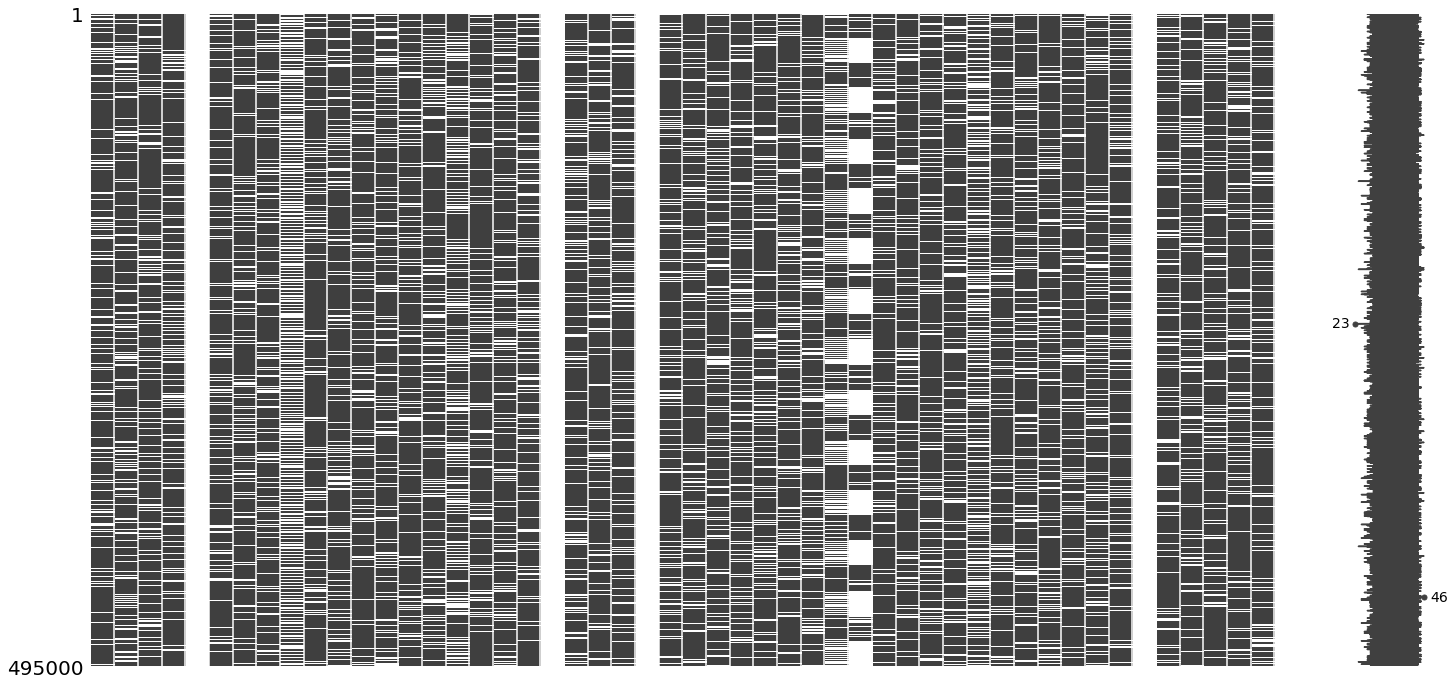
\includegraphics[width = 0.6\textwidth]{chapter3/missing.png}
  \caption{缺失值处理后数据分布情况}
  \end{figure}

试验结果表明模型在存在缺失值的况下都 发生性能的下降,其中 USAD 模型的性能损失最 多,GDN模型的性能下降最少。经过调查发现,USAD 模型是基于数据整体分布建模并重建的方法,缺失值的引入影响了模型对非缺失值数据的建模与重建,致使模型性能下降;GDN 是面向多元时间序列间关联性建模的方法,其更侧重于从数据中学习不同维度的时间序列之间关联性,在一定数据缺失的情况仍然能够鼓励模型学习多元时间序列之间的关联性。但尽管如此,GDN 模型的性能仍然在 beta = 0.3 和 beta = 0.5 的场景下相比原性能下降了 26\% 和 28\%。

\begin{figure}[ht]
    \centering
    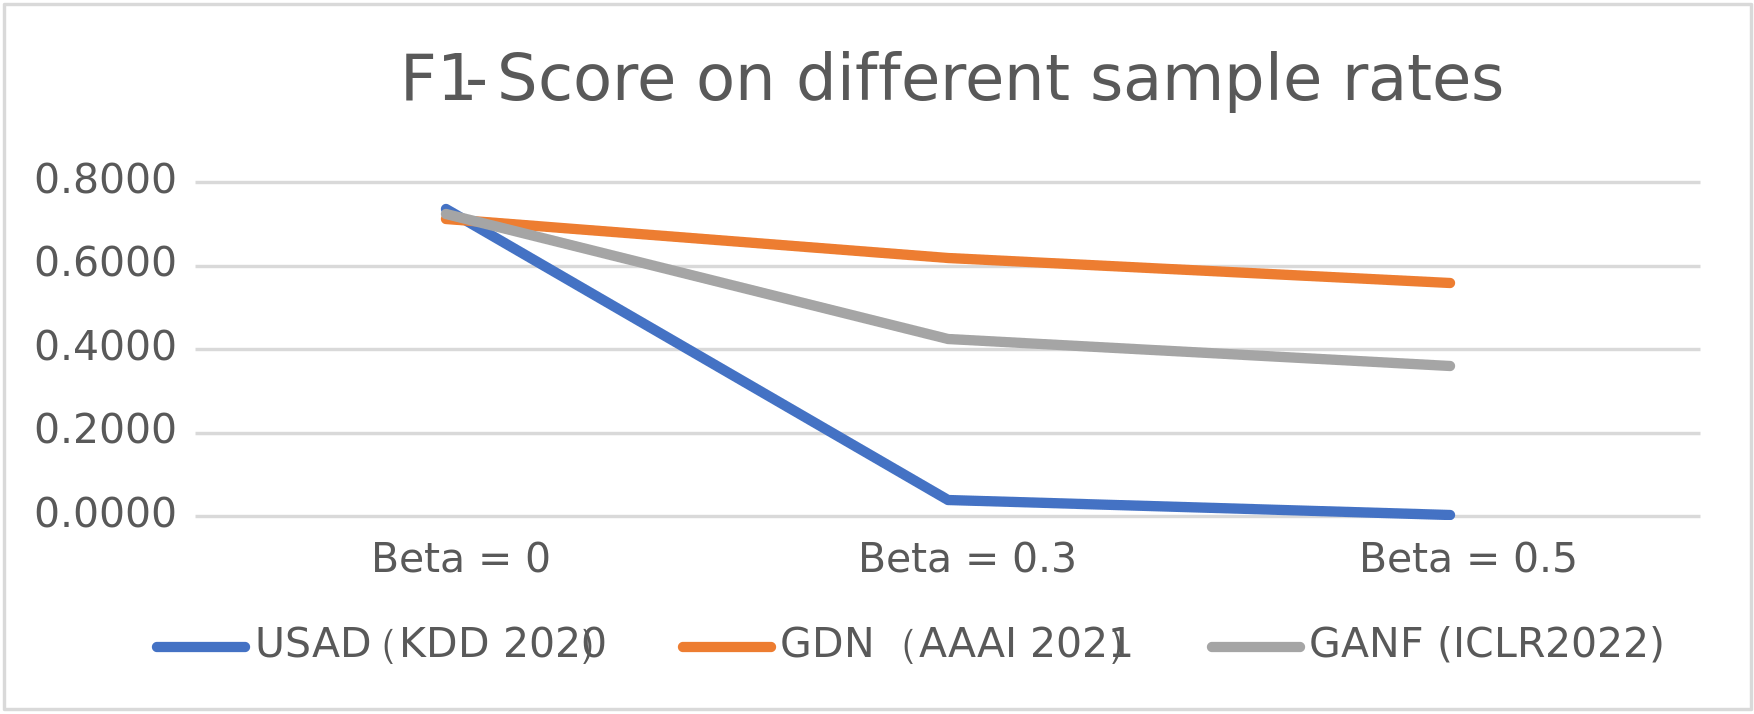
\includegraphics[width = 0.8\textwidth]{chapter3/compare1.png}
    \caption{缺失值场景下SOTA模型性能表现}
    \end{figure}
  
  综上我们可得到结论,传统 SOTA 模型在我 们模拟的缺失值新场景下性能会发生较大下降, 无法满足真实场景下存在缺失值时的性能需求。 如何保证多元时间序列异常检测模型在存在缺失 值的场景下依然能够保证良好的性能具有重要的现实意义。


\section{基于注意力机制重新表征的缺失值时间序列异常检测}[Introduction]
综上,本章预计提出如下贡献点:

提出一种面向缺失值的多元时间序 列的异常检测算法MMAD (Missing Multi Time Series Anomaly Detection),该算法首次提出了一种缺失值场景下的多元时间序列异常检测解决方案。

提出的一种掩码注意力机制模块 (MMAR)将包含缺失值的不完整时间序列数据映射为完整的高维嵌入表征,该表征融合了时间信息、缺失值信息以及观测值信息;同时提出一种基于条件标准化流的标准化分布变换模块(CNF-AD)对该表征进行重建,该模块学习一个可逆变换函数实现一个简单分布(例如高斯分布)与真实分布近似之间的映射,通过该函数与简单分布计算观测值在真实分布中的近似概率,以该概率作为异常分数进行异常检测。

实验结果表明我们的方法在多维时间序 列异常检测任务上有着良好的表现,同时在不规 则时间序列的任务上超越了当前传统异常检测方法。

\begin{figure}[htb]
  \centering
  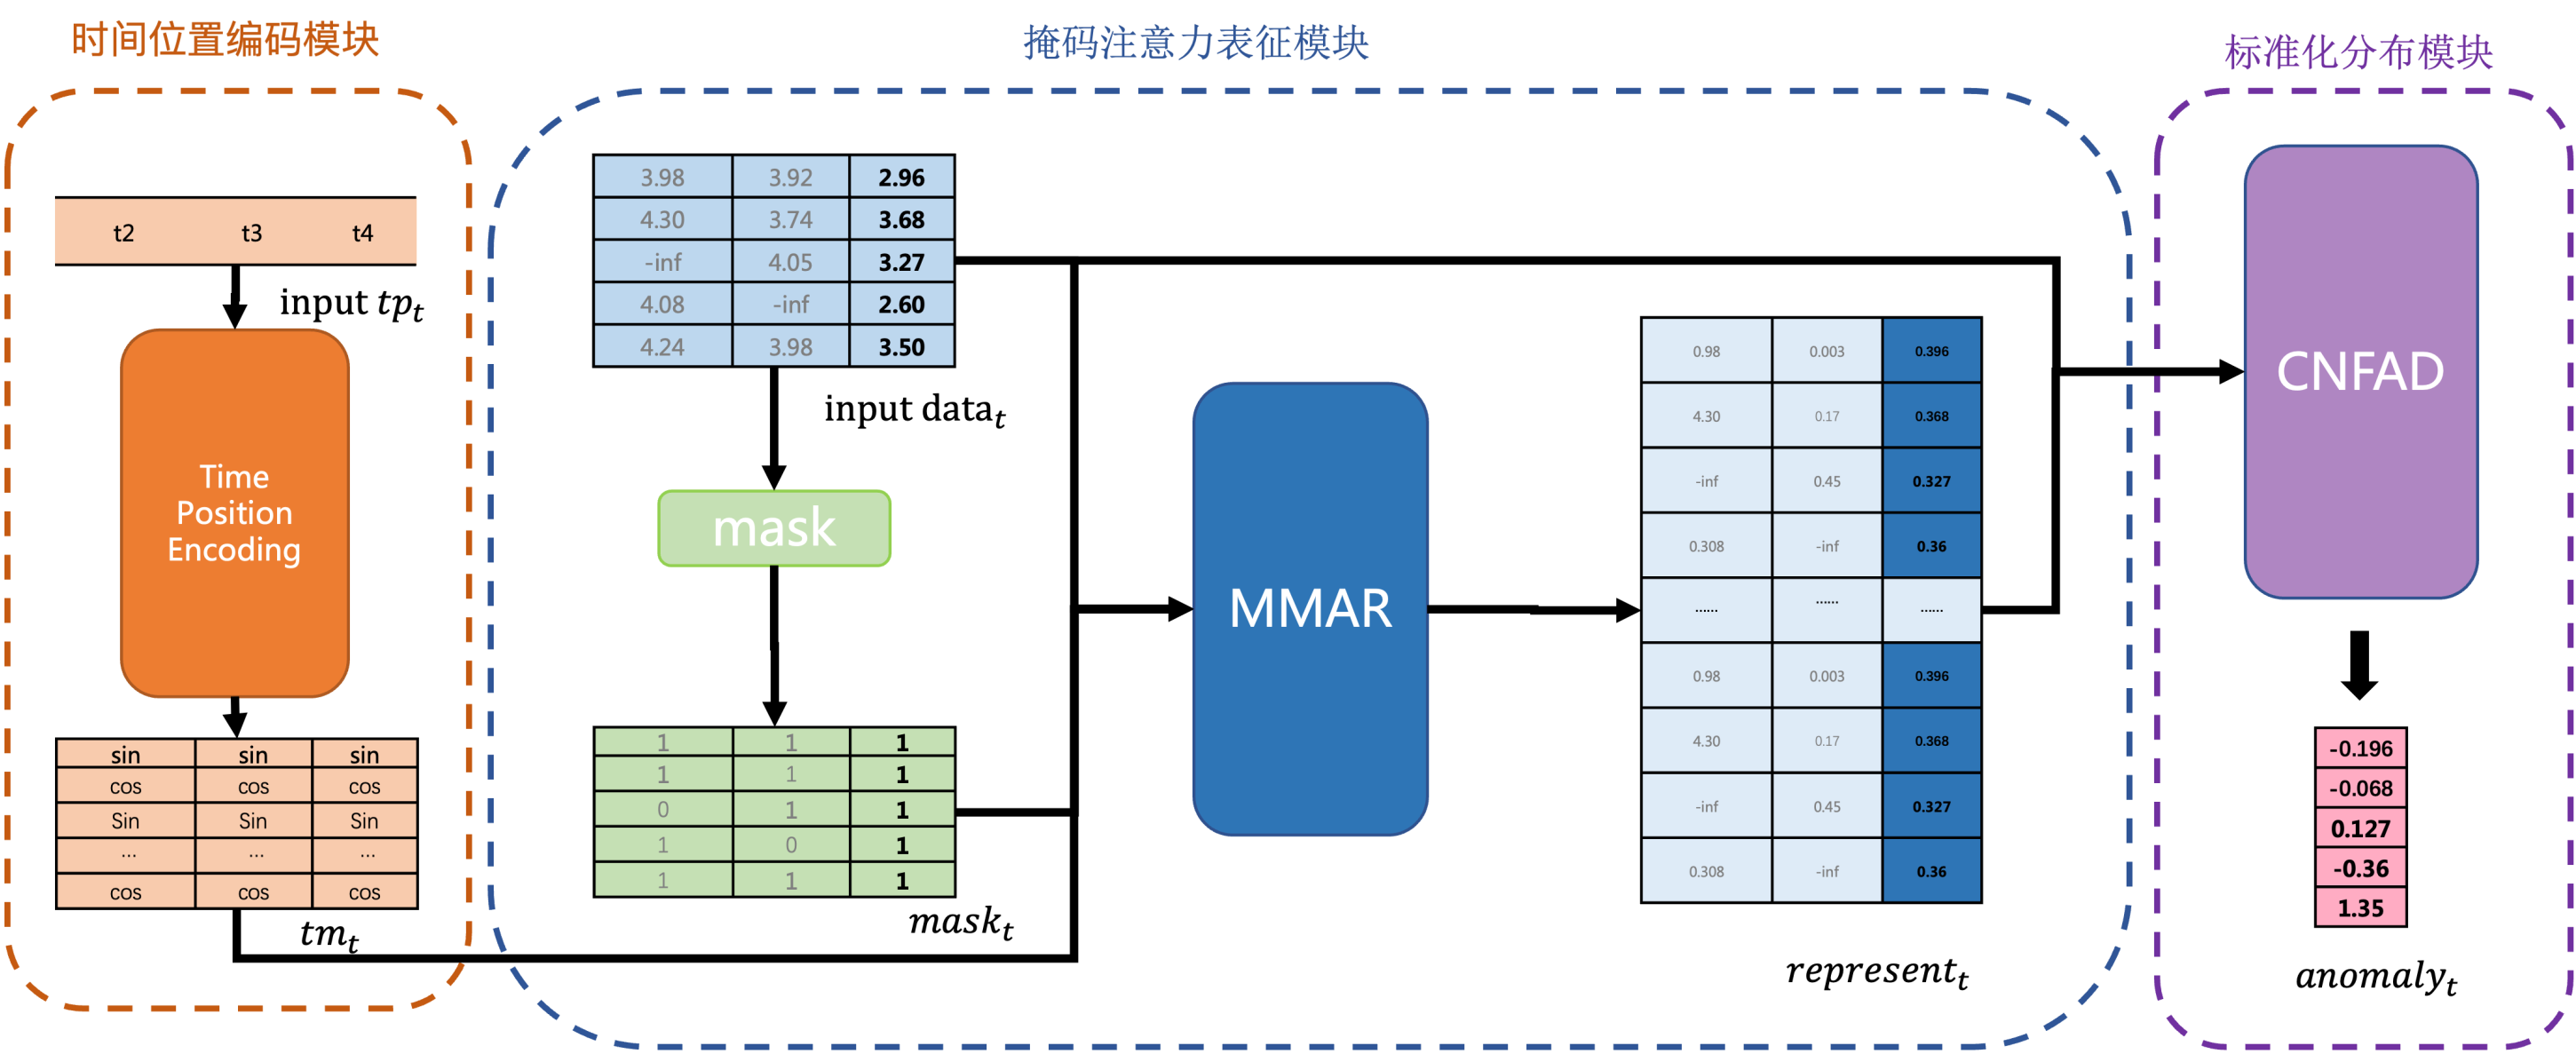
\includegraphics[width = 1\textwidth]{chapter3/overview.png}
  \caption{模型整体架构}
  \end{figure}

模型主要由三个模块组成,即时间位置编码模块(Time Position Encoding)、掩码注意力表征模块(MMAR)和标准化分布变换模块(CNF-AD)。
其中时间位置编码模块的主要目的是将原时间向量$tp_t$ 转换成时间矩阵 $timematrix_t$以建模不同时刻之间的关联关系;掩码注意力表征模块(MMAR) 主要目的是将包含缺失值的不完整时间序列数据映射为完整的高维嵌入表征;标准化分布变 换模块(CNFAD)的目的是学习一个可逆变换函数实现一个简单分布(例如高斯分布)与真实分布近似之间的映射,通过该函数与简单分布计算观测值在真实分布中的近似概率,以该概率作为异常分数进行异常检测。
\subsection{时间位置编码模块}

  时间位置编码模块主要对时间戳进行重新编码,将原来由单个数值的时间戳编码到$d_model$长度的向量以表示更加丰富的信息。对于原来$(t_2,t_3,t_4)$的 $tp_t\in R^{1 x L}$, 所组成的时间戳向量我们会通过位置编码来映射到$timematrix_t$矩阵中。
  \begin{figure}[ht]
    \centering
    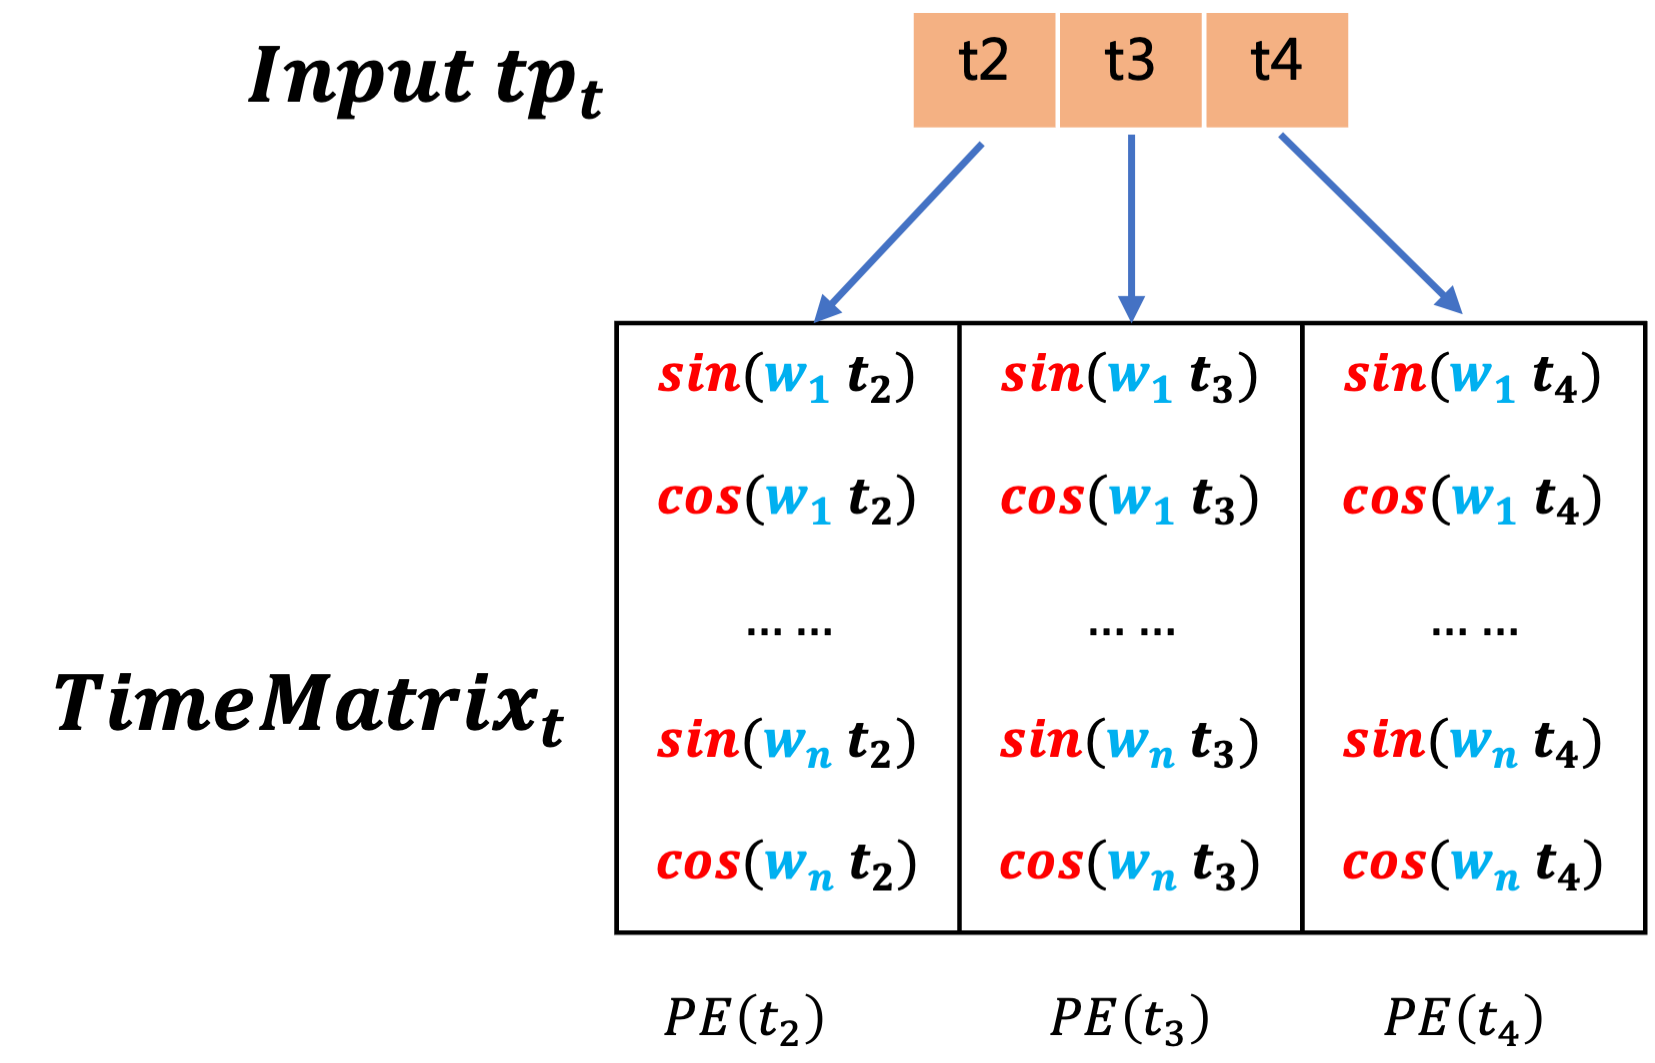
\includegraphics[width = 0.6\textwidth]{chapter3/time1.png}
    \caption{时间向量转化为时间矩阵}
    \end{figure}
  
  
  
  以上图为例子, 原始时间倠是如同“ $2022 / 5 / 13$ 15:03:00” 的格式化日期时间, 首先会将其转化成 UNINX 整数型时间戳 “ 16524380 ” 并作为变量 $t$ 。 通过给时间 $t$ 设置不同的参数 $\frac{1}{1 e 5^{\frac{2 i}{d_{\text {model }}}}}$, 其中 $i$ 为 向量中的标号, $\left(i=0,1, \ldots, \frac{d_{\text {model }}}{2}-1\right) \in(0,1)$ 。
  
  对于不同时刻的同一维度参数相同,我们可 以通过正余弦和公式来推导不同时刻之间的相对 与绝对位置关系:
  \begin{equation}
    \begin{aligned}
    \sin (t+p) &=\sin (t) \cos (p)+\cos (t) \sin (p) \\
    \cos (t+p) &=\cos (t) \cos (p)-\sin (t) \sin (p)
    \end{aligned}
    \end{equation}
  绝对位置关系指的是某时刻 $t$ 与其距离绝对 位置 $p$ 的关系, 由于 $p$ 在此处是一个常数故我 们可以将 $P E(t+p)$ 写成一个关于 $P E(t)$ 和常 数 $P E(p)$ 线性组合:
  \begin{equation}
    P E(t+p)=\alpha P E(t)+\beta P E(p)
    \end{equation}
  对于在后续的注意力机制计算中, 两个不同位置 的关系将通过点积来对其表示, 所以相对位置关 系指的是 $P E(t+p)$ 与 $P E(t)$ 之间的点积。同理 由上面的推导我们也能将 $P E(t+p) P E(t)$ 写成 一个关于 $P E(t)$ 和常数 $P E(p)$ 线性组合:
    \begin{equation}
      P E(t+p) P E(t)=(\alpha P E(t)+\beta P E(p)) P E(t)
    \end{equation}
  
  \begin{figure}[ht]
    \centering
    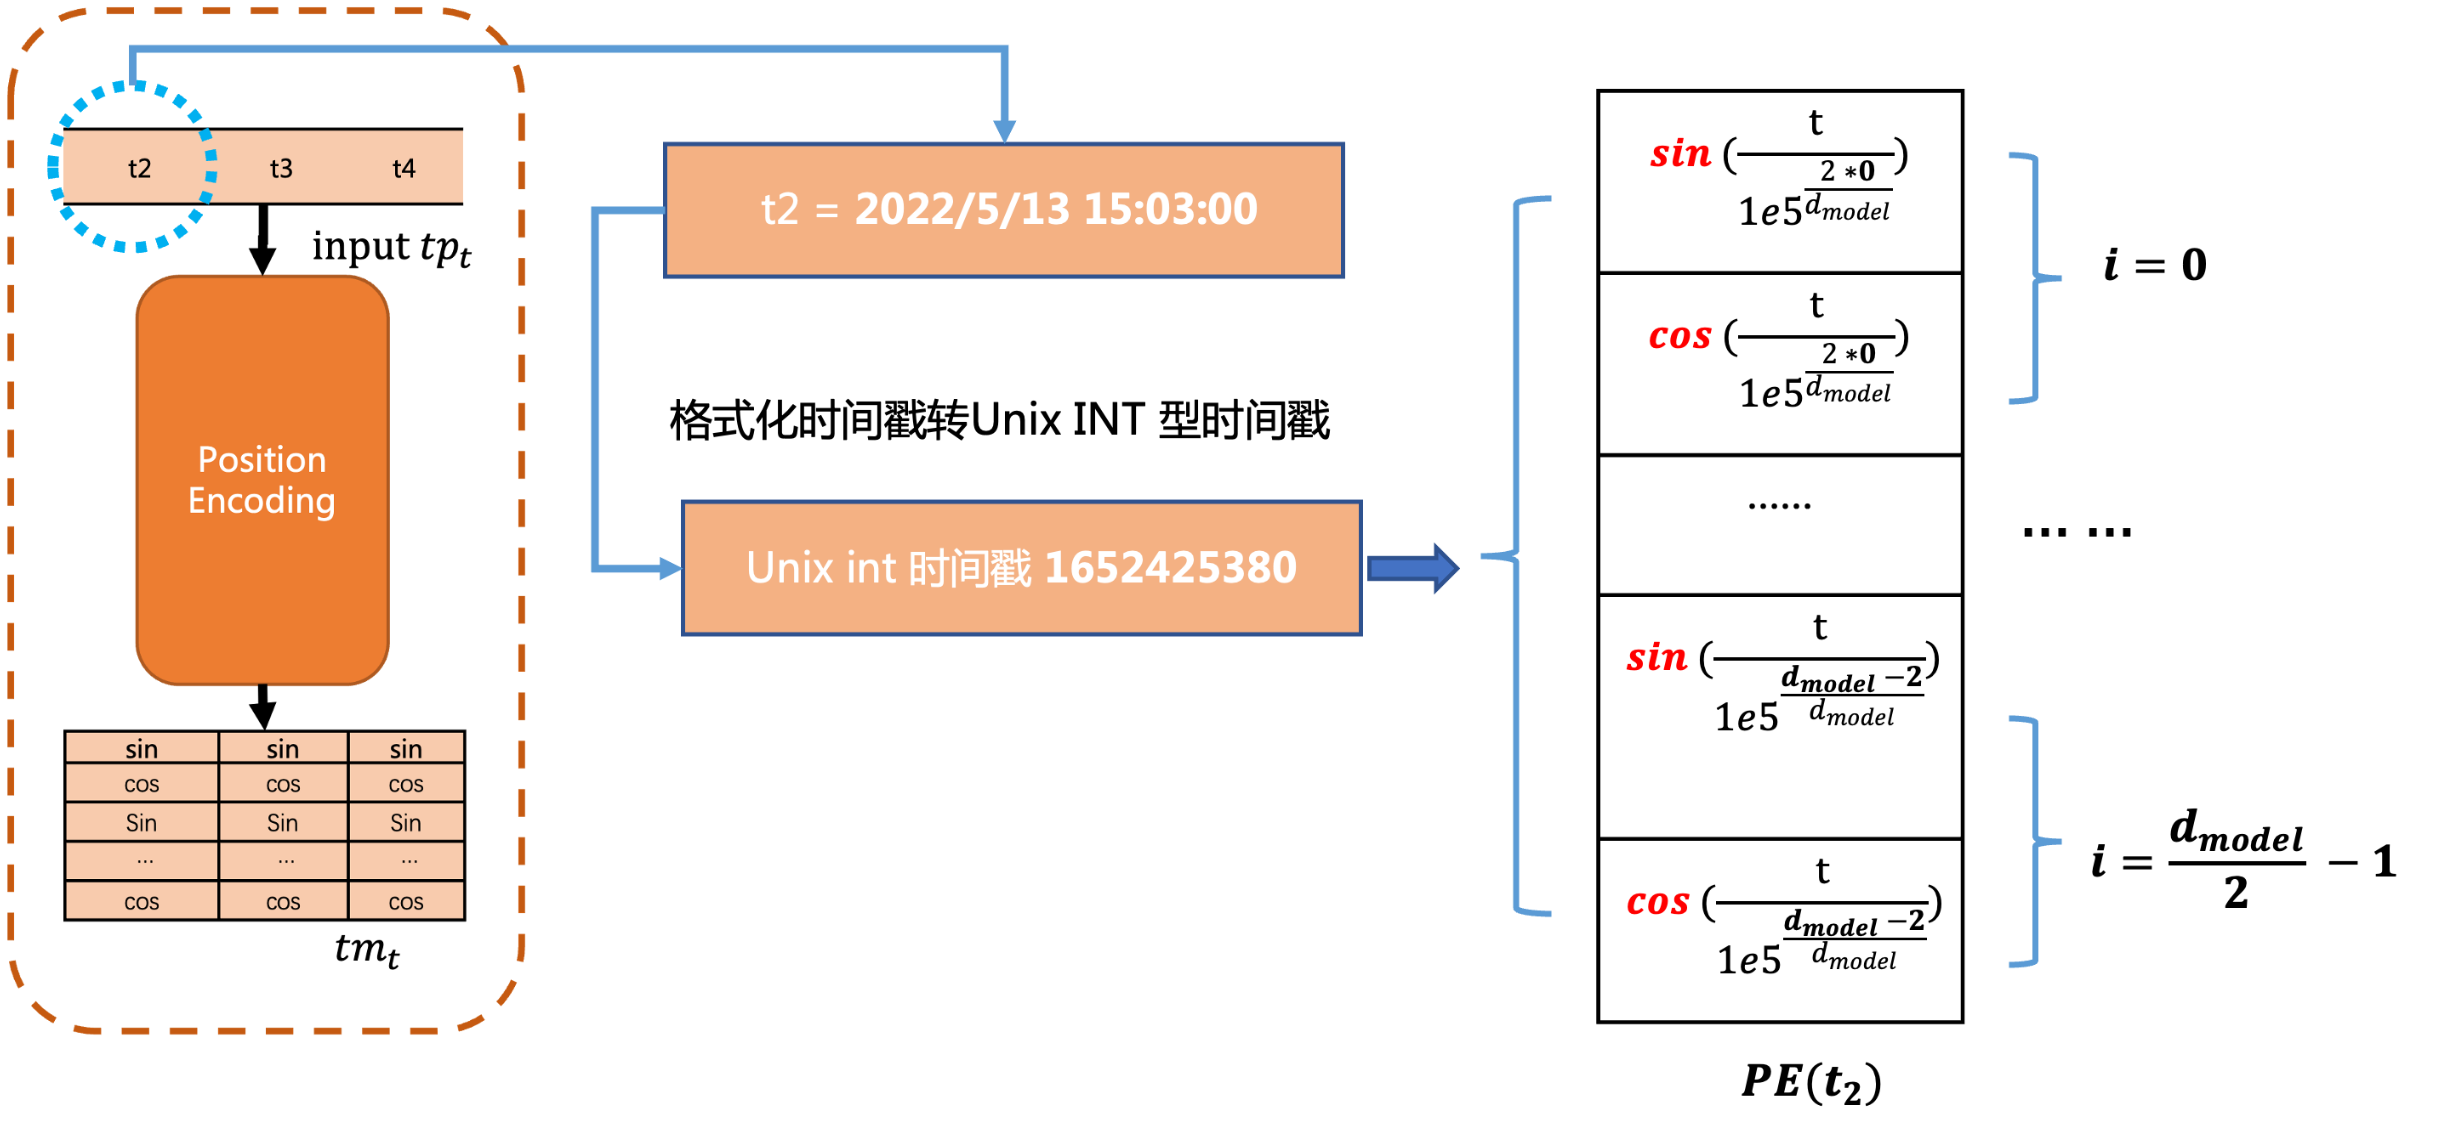
\includegraphics[width = 1\textwidth]{chapter3/time2.png}
    \caption{单个时间戳转换流程}
    \end{figure}
  
  \subsection{掩码注意力表征模块}
  这一模块的主要目的是通过真实数据 $data_t$, 缺失值分布矩阵 $mask_t$, 以及由上一模块所计算 得到的时间矩阵 $timematrix_t$ 来计算得到 的关系,$timematrix $中不同时刻之间的关系, $mask_t$ 中缺失值与非缺失值之间的关系,并用于 后续基于标准化流异常检测的推断。
  
  \begin{figure}[ht]
    \centering
    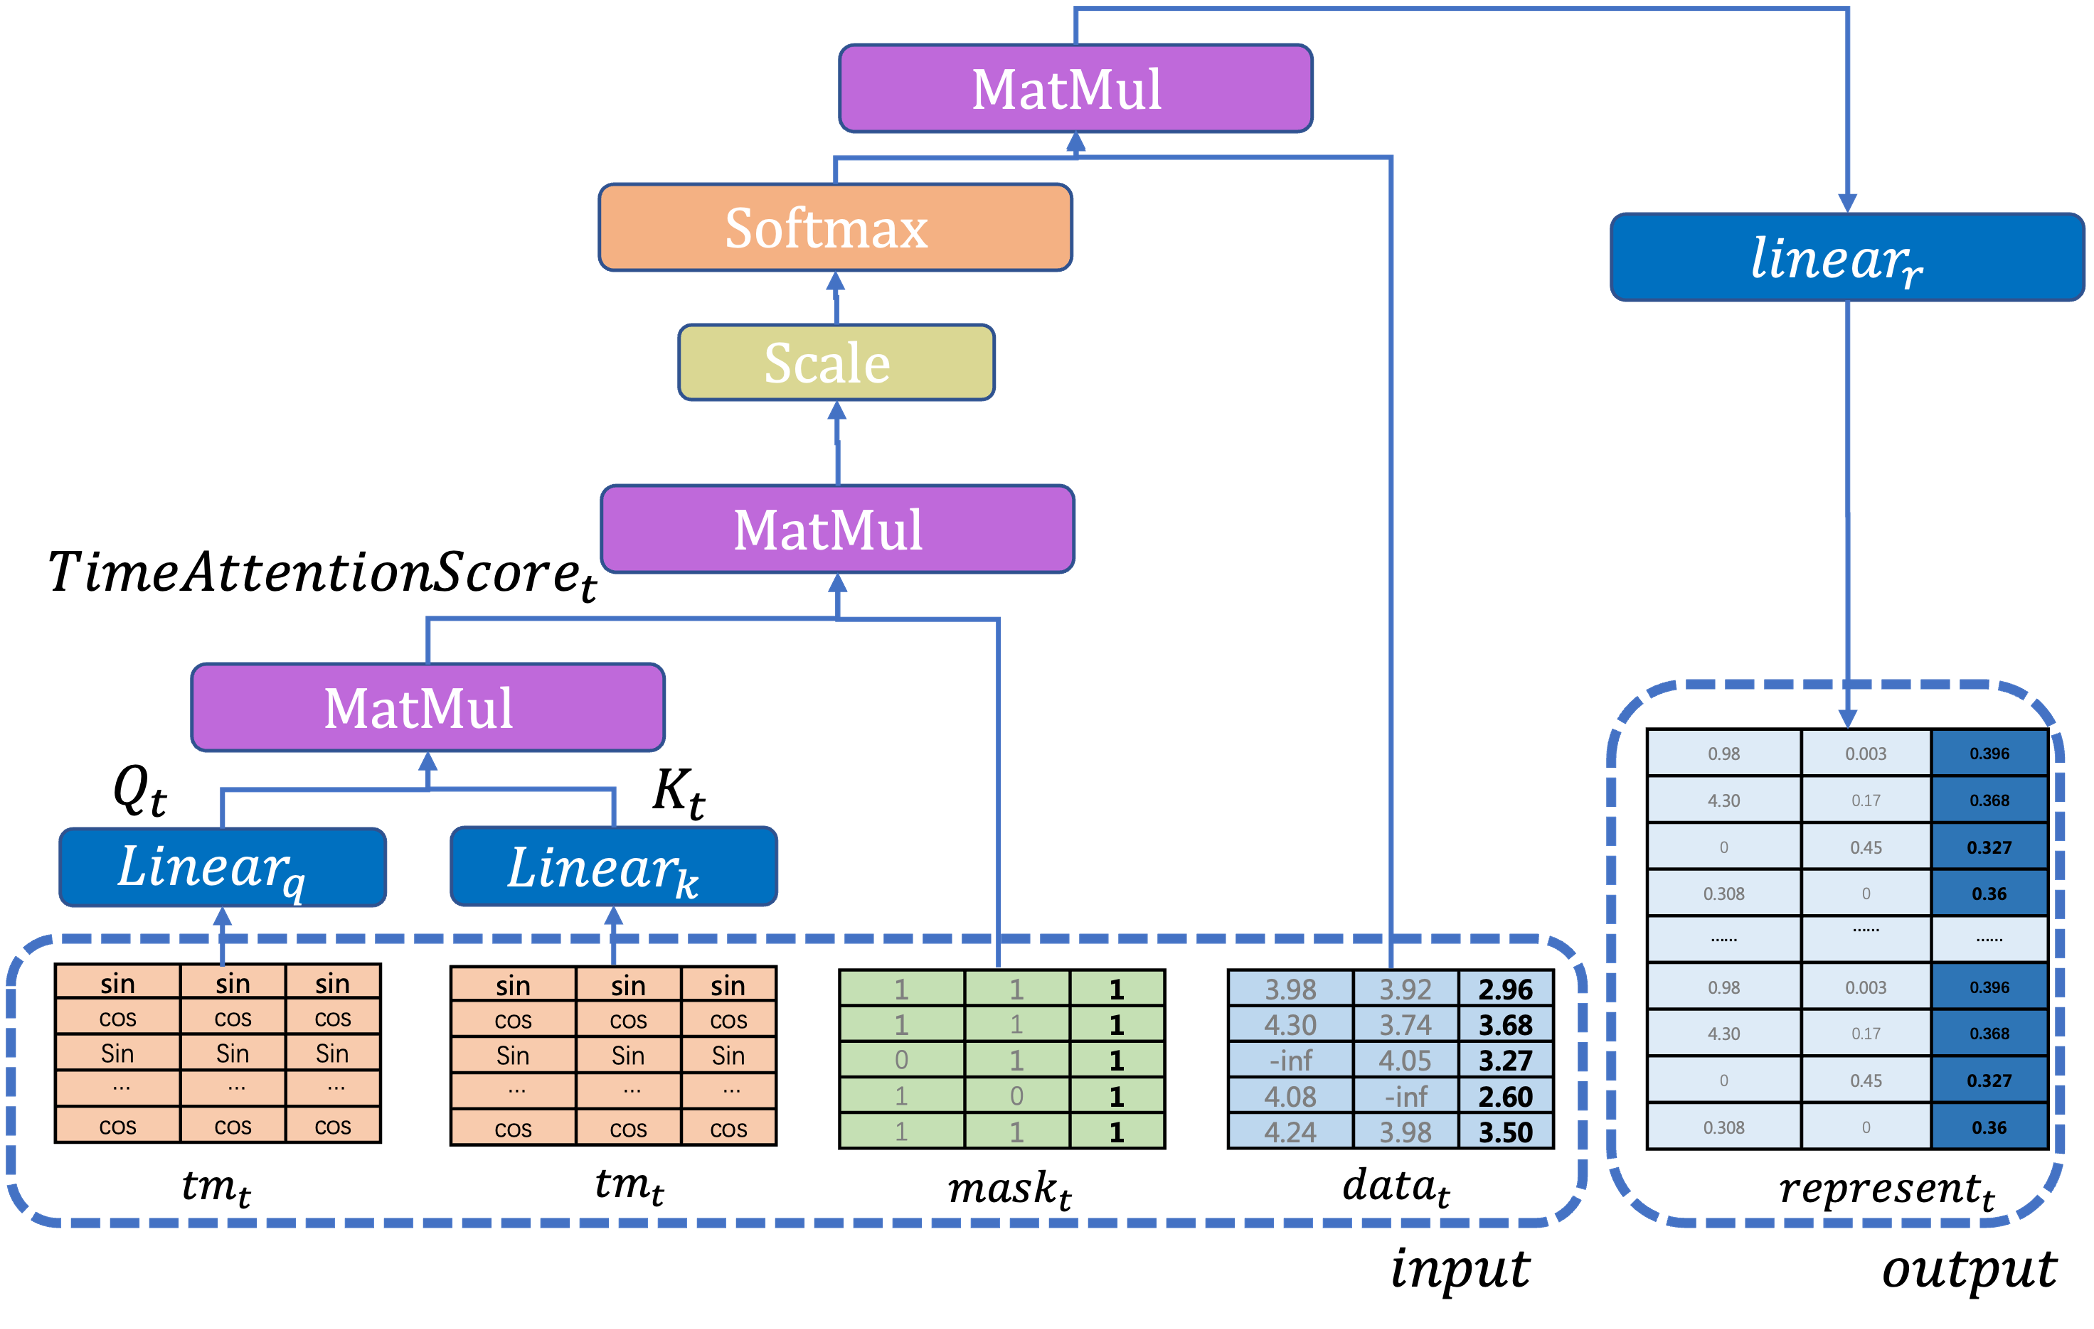
\includegraphics[width = 0.8\textwidth]{chapter3/mask.png}
    \caption{掩码注意力表征模块架构}
    \end{figure}
  
  由上图我们可以看到 MMAR 的细节。MMAR 以$timematrix_t$, $mask_t$, $data_t$ 作为输 入, $represen_t$ 作为输出。
  
  第一步, 通过两个独立线形层$linear_q$,$linear_k$将$timematrix_t$转化为$Q_t, K_t$ 矩阵, 并计根据公式 $\frac{Q_t K_t^T}{\sqrt{d}}$, 计算得到 $TimeAttentionScore_t$, 其中 $d$ 是注意力机制所 到了不同时刻之间的注意力权重。
  
  第二步,融入缺失值信息。首先模型会通过mask模块将$data_t$中的缺失值和非缺失值值进行提取,并用0,1 (0 代表缺失值,1 代表非缺失值)代替得到$mask_t$, 将$mask_t$与刚才与上一步中$TimeAttention_t$ 融合得到最终的面向缺失值注意力分数$maskTimeAttentionScore_t$。
  
  第三步,融入真实数据信息。通过将包含了不同时刻上下文的真实数据 $data_t$ 与包含了不同时刻$maskTimeAttensionScore_t$  进行融合以对$data_t$ 进行重新表征,这一步的目的主要是学习到$data_t $在时间维度上的的主要分布。
  
  第四步,我们利用一个线性层$linear_r$将上一步得到的$maskTimeAttentionData_t$ 映射到高维空间即 
  \begin{equation}
    represent_t=linear_r(maskTimeAttentionData_t)
  \end{equation}
  
  \subsection{标准化分布变换模块}
  \begin{figure}[ht]
    \centering
    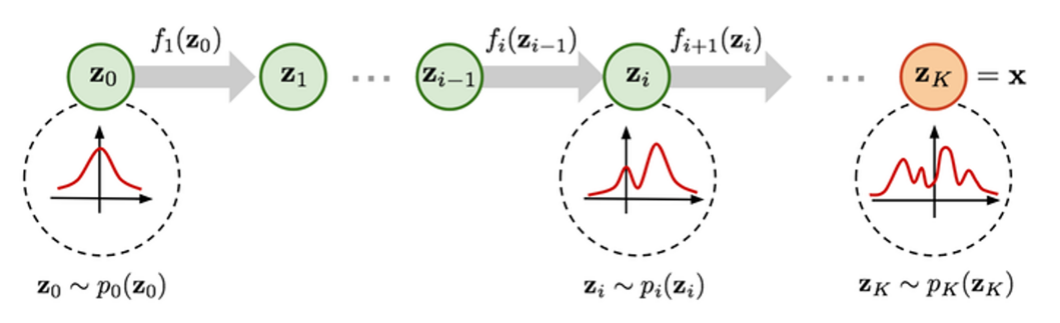
\includegraphics[width = 1\textwidth]{chapter3/nf2.png}
    \caption{标准化流原理解释}
    \end{figure}
  
  在获取到$represent_t$之后,我们需要依据这些信息对观测值进行是否异常的判断。传统异常检测方法往往基于AE, VAE 等生成模型对生 成的编码进行重构,并用生成数据与真实真实数 据的差异作为异常分数,这种方式最大对于生成 模型的输入编码要求很高,需要非常准确的捕捉 到数据的真实分布。
  我们采用了一种基于标准化流的异常检测模 型并加以改进,标准化流并不直接生成真实数据,而是尝试学习一种变换,将类似于正态分布等简 单分布进行一系列的可逆变换以逼近真实的数据分布。
  如图所示
  
  \begin{figure}[ht]
    \centering
    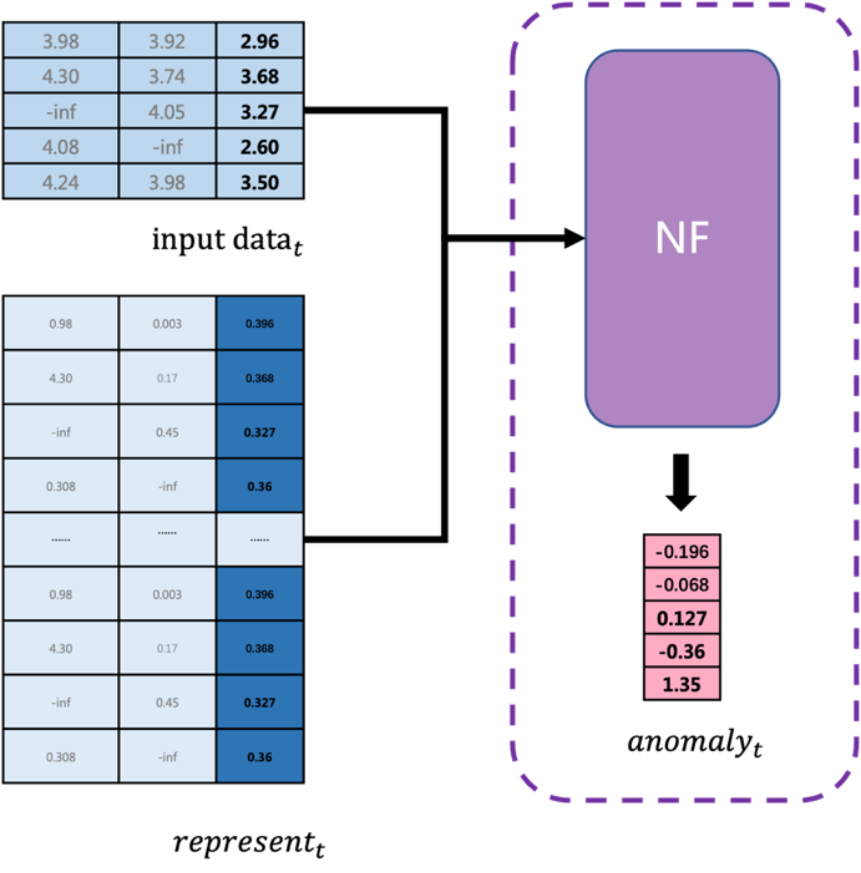
\includegraphics[width = 0.6\textwidth]{chapter3/nf1.png}
    \caption{标准化分布变换模块架构}
    \end{figure}
  
  据概率密度的变换定理,如果$y =f(x) $且 $f$ 是可逆的那么存在:
  \begin{equation}
    \begin{gathered}
    p_x(x)=p_y(f(x)) *|\operatorname{det} J f(x)| \\
    p_y(y)=p_x\left(f^{-1}(y)\right) *\left|\operatorname{det} J f^{-1}(y)\right|
    \end{gathered}
    \end{equation}
  
  如果存在多个可逆 $f$ , 那么在取log 后进行加和
    \begin{equation}
      \begin{gathered}
      z_k=f_k \circ \ldots \circ f_2 \circ f_1\left(z_0\right) \\
      \log _q\left(z_k\right)=\log _{q 0} z_0-\sum_{k=1}^K \log \operatorname{det}\left|\frac{\partial f_k}{\partial z_k}\right|
      \end{gathered}
      \end{equation}
  
  进一步的,我们可以将标准流推广到条件标准化流, 即:
  \begin{equation}
    \log _p(x \mid h)=\log _q(f(x ; h))+\log \left|\operatorname{det} \nabla_x f(x ; h)\right|
    \end{equation}
  
  简单来讲, 在真实分布 $p$ 上取得在满足限制条件 $h$ 的数据 $\mathrm{x}$ 的概率密度 $\log$ 值可以等价于在简单 分布 $q$ 上取得变换后 $f(x ; h)$ 的概率密度 $\log$ 值加上 余项 $\log \left|\operatorname{det} \nabla_x f(x ; h)\right|$ 。
  
  \subsection{训练过程及异常分数设置}
  我们将数据在真实分布上概率密度的log值设为异常分数,令$represent_t$作为当前$data_t$的限制条件,故我们的异常分数设置为:
  
  \begin{equation}
    \begin{aligned}
    &\text { Anomal }_t=\log p\left(\text { data }_t \mid \text { represent }_t\right) \\
    &=\log q\left(f\left(\text { data }_t ; \text { represent }_t\right)\right) \\
    &+\log \mid \operatorname{det} \nabla_{\text {data }_t} f\left(\text { data }_t ; \text { represent }_t\right) \mid
    \end{aligned}
    \end{equation}
  
  其中 $p$ 是真实数据的分布,$q$ 为一种简单分布,例如高斯分布或均匀分布,$f$ 为模型训练得到的可逆变换。
  在多元时间序列异常检测问题中,训练集通常被设置为不存在攻击或异常的时间段所收集的数据;测试集通常被设置为存在攻击或异常的时间段的数据。所以我们的训练目标是使的训练集上的异常分数最小,故我们使用最大似然估计(MLE)作为我们的损失函数:
  
  \begin{equation}
    \begin{aligned}
    &\min G(X) \\
    &=-\sum_{t=1}^{L_{\text {train }}} \log q\left(f\left(\text { data }_t ; \text { represent }_t\right)\right) \\
    &+\log \mid \operatorname{det}_{\text {data }_t} f\left(\text { data }_t ; \text { represent }_t\right) \mid
    \end{aligned}
    \end{equation}

\section{实验结果及分析}[Introduction]
\subsection{实验数据集}
\textbf{SWAT数据集}\cite{swat}: SWaT数据源于与新加坡公用事业委员会协调的运行水处理试验台。该数据以1秒的频率收集持续11天的51个传感器记录。该数据集分为测试集和训练集,其中前7天为训练集,不包含异常或攻击行为,后4天为测试集合,总共进行了36次攻击,其中大约11\%的时间步为异常标签。

\textbf{WADI数据集}: WADI是一个由大量供水管道组成的供水系统。因此,WADI形成了一个更加完整和现实的水处理,存储和分配网络。数据集包含14天正常运行数据,这些数据组成了训练集、在接下来的几天,以不同的时间间隔进行了许多受控的物理攻击,这与测试集中的异常情况对应。

\textbf{SMD数据集}: SMD是从一家大型互联网公司收集的服务器机器数据集,数据集被分为两个等长的部分,其中前半部分为没有发生异常的数据集,可以被用来作为训练集;后半部分包含攻击行为,可以被用来作为测试集。

\subsection{实验设置}

真实世界中往往会因为传输条件的限制,传感器的自然损坏而没有被及时更换等情况而导致数据的缺失,为了模拟真实的数据缺失情况,我们在每个传感器的时间维度上进行均匀采样,并删除采样时间戳上的数据。

在介绍评价指标之前,需要先介绍混淆矩阵。在机器学习领域,混淆矩阵(Confusion Matrix),又称为可能性矩阵或错误矩阵。混淆矩阵是可视化工具,特别用于监督学习,在无监督学习一般叫做匹配矩阵。主要用于比较分类结果和实际测得值,可以把分类结果的精度显示在一个混淆矩阵里面。
混淆矩阵的每一列代表了预测类别,每一列的总数表示预测为该类别的数据的数目;每一行代表了数据的真实归属类别,每一行的数据总数表示该类别的数据实例的数目;每一列中的数值表示真实数据被预测为该类的数目。
其中主要包含四个参数:True Positive(TP):真正类。样本的真实类别是正类,并且模型识别的结果也是正类。False Negative(FN):假负类。样本的真实类别是正类,但是模型将其识别为负类。 False Positive(FP):假正类。样本的真实类别是负类,但是模型将其识别为正类。True Negative(TN):真负类。样本的真实类别是负类,并且模型将其识别为负类。

\begin{figure}[ht]
  \centering
  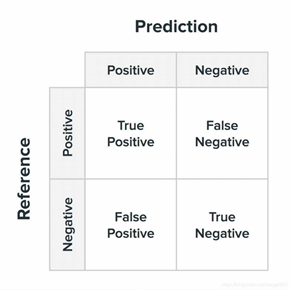
\includegraphics[width = 0.4\textwidth]{chapter4/confusematrix.png}
  \caption{混淆矩阵}
  \end{figure}

多元时间序列异常检测模型一般采用Precision,Recall,F1-Score 作为性能评价指标。其中Precision是检测出某类特征的数量与检测出的所有特征数量之间的比率,衡量的是模型的查准率;一般来说,Precision就是检索出来的条目有多少是准确的。Recall是指检测出的某类特征的数量和数据集中所有的该类特征数量的比率,衡量的是检索系统的查全率。

公式(4-1),公式(4-2),公式(4-3)分别列出了精确度Precision,召回率Recall,F1-Score 的计算方式
\begin{equation}
  \text { Precession }=\frac{T P}{T P+F P}
  \end{equation}

\begin{equation}
  \text { Recall }=\frac{T P}{T P+F N}
  \end{equation}

  \begin{equation}
  F 1=\frac{2 * \text { Precision } * \text { Recall }}{\text { Precision }+\text { Recall }}
  \end{equation}

\subsection{基线模型说明}
\textbf{USAD(Audibert 等,KDD 2020)}采用的是无监督异常检测,在两阶段训练方案下训练两个自动编码器,包括一个共享编码器和两个单独的解码器:自动编码器训练阶段和对抗训练阶段。

\textbf{GDN(Deng 等,AAAI  2021)}采用的是无监督异常检测,将结构学习方法与图形神经网络相结合,着重建模不同维度时间序列之间的关系,另外使用注意力权重来解释检测到的异常。

\textbf{GANF(DAI 等,ICLR  2022)}采用的是无监督异常检测。通过贝叶斯网络建模因果关系的有向无环图(DAG), 通过RNN建模时间序列;引入条件概率作为检测异常分数。

\subsection{总体性能对比}
如表4-1, 表4-2, 表4-3所示,我们测试了不同程度下删除数据后模型性能表现。通过实验结果我们可以看到,我们在SOTA模型的原场景下接近SOTA的性能,
同时在我们设计的新的场景下超过SOTA模型的表现,以此可以证明我们的模型在缺失值场景下具有较好的性能表现。
同时我们的模型在beta = 0 至 beta = 0.3 与 beta = 0.3 至 beta = 0.5 的场景变换中,性能下降最低,这证明了我们的模型在数据损失的情况下性能
下降最不明显,对数据缺失具有鲁棒性。

\begin{table}[htb]
  \caption{所有方法在SWAT数据集上的性能比较}
  %\label{comparison_results}
  \small
  \centering
  \setlength{\tabcolsep}{0.8mm}{
  \begin{tabular}{lccccccccc}\toprule
  Method & \multicolumn{3}{c}{SWAT FULL DATA} & \multicolumn{3}{c}{SWAT DROP 0.3 DATA} & \multicolumn{3}{c}{SWAT DROP 0.5 DATA} \\ \cmidrule(r){2-4} \cmidrule(r){5-7} \cmidrule(r){8-10}
      & F1-Score & Precision & Recall & F1-Score & Precision & Recall & F1-Score & Precision & Recall\\ \midrule
  USAD & 0.7917 & 0.9851 & 0.6618  & 0.5635 & 0.4238 & 0.8408  & 0.3636 & 0.2456 & 0.7003 \\
  GDN & 0.8100 & 0.9935 & 0.6812  & 0.6609 & 0.8167 & 0.5550  & 0.5666 & 0.7271 &  0.4641 \\
  GANF & 0.8065 & 0.9892 & 0.6808  & 0.3048 & 0.2025 & 0.6154  & 0.1314 & 0.0703 &  1.0000 \\
  MMTSAD & 0.7522 & 0.9583 & 0.6191  & 0.6886 & 0.8106 & 0.5986  & 0.6869 & 0.784  & 0.6112 \\
%\bfseries MUSE-Net& \bfseries 2.89 & \bfseries 1.10 & \bfseries 2.74 & \bfseries 1.05 & \bfseries 15.47 & \bfseries 5.47 & \bfseries 14.45 & \bfseries 5.54 & \bfseries 17.19 \\
\bottomrule
\centering
\end{tabular}}
\end{table}


\begin{table}[htb]
  \caption{所有方法在WADI数据集上的性能比较}
  %\label{comparison_results}
  \small
  \centering
  \setlength{\tabcolsep}{0.8mm}{
  \begin{tabular}{lccccccccc}\toprule
  Method & \multicolumn{3}{c}{WADI FULL DATA} & \multicolumn{3}{c}{WADI DROP 0.3 DATA} & \multicolumn{3}{c}{WADI DROP 0.5 DATA} \\ \cmidrule(r){2-4} \cmidrule(r){5-7} \cmidrule(r){8-10}
      & F1-Score & Precision & Recall & F1-Score & Precision & Recall & F1-Score & Precision & Recall\\ \midrule
  USAD & 0.2328 & 0.9947 & 0.1318 & 0.2137 & 0.2551 & 0.1838  & 0.1866 & 0.1897 & 0.1836 \\
  GDN & 0.5700 & 0.9750 & 0.4019  & 0.1389 & 0.0802 & 0.5177  & 0.1092 & 0.1092 & 1.0000 \\
  GANF & 0.3348 & 0.2040 & 0.9324  & 0.2234 & 0.1396 & 0.5584  & 0.1739 & 0.1667 & 0.1818 \\ 
  MMTSAD & 0.3897 & 0.2718 & 0.6883  & 0.2821 & 0.2102 & 0.4286  & 0.2179 & 0.2179 & 0.5844 \\ 
%\bfseries MUSE-Net& \bfseries 2.89 & \bfseries 1.10 & \bfseries 2.74 & \bfseries 1.05 & \bfseries 15.47 & \bfseries 5.47 & \bfseries 14.45 & \bfseries 5.54 & \bfseries 17.19 \\
\bottomrule
\centering
\end{tabular}}
\end{table}

\begin{table}[htb]
  \caption{所有方法在SMD数据集上的性能比较}
  %\label{comparison_results}
  \small
  \centering
  \setlength{\tabcolsep}{0.8mm}{
  \begin{tabular}{lccccccccc}\toprule
  Method & \multicolumn{3}{c}{SMD FULL DATA} & \multicolumn{3}{c}{SMD DROP 0.3 DATA} & \multicolumn{3}{c}{SMD DROP 0.5 DATA} \\ \cmidrule(r){2-4} \cmidrule(r){5-7} \cmidrule(r){8-10}
      & F1-Score & Precision & Recall & F1-Score & Precision & Recall & F1-Score & Precision & Recall\\ \midrule
      USAD & 0.9382 & 0.9314 & 0.9617  & 0.6129 & 0.4713 & 0.8762  & 0.5818 & 0.4392 & 0.8617 \\
      GDN & 0.7183 & 0.7079 & 0.7294  & 0.6263 & 0.5955 & 0.6607  & 0.3517 & 0.2364 & 0.6871 \\ 
      GANF & 0.6241 & 0.5131 & 0.7963  & 0.5983 & 0.4779 & 0.8000  & 0.5808 & 0.4247 & 0.9185 \\ 
      MMTSAD & 0.7949 & 0.9051 & 0.7086  & 0.7025 & 0.7367 & 0.6714  & 0.6491 & 0.5881 & 0.7243 \\
%\bfseries MUSE-Net& \bfseries 2.89 & \bfseries 1.10 & \bfseries 2.74 & \bfseries 1.05 & \bfseries 15.47 & \bfseries 5.47 & \bfseries 14.45 & \bfseries 5.54 & \bfseries 17.19 \\
\bottomrule
\centering
\end{tabular}}
\end{table}

\begin{figure}[htb]
  \centering
  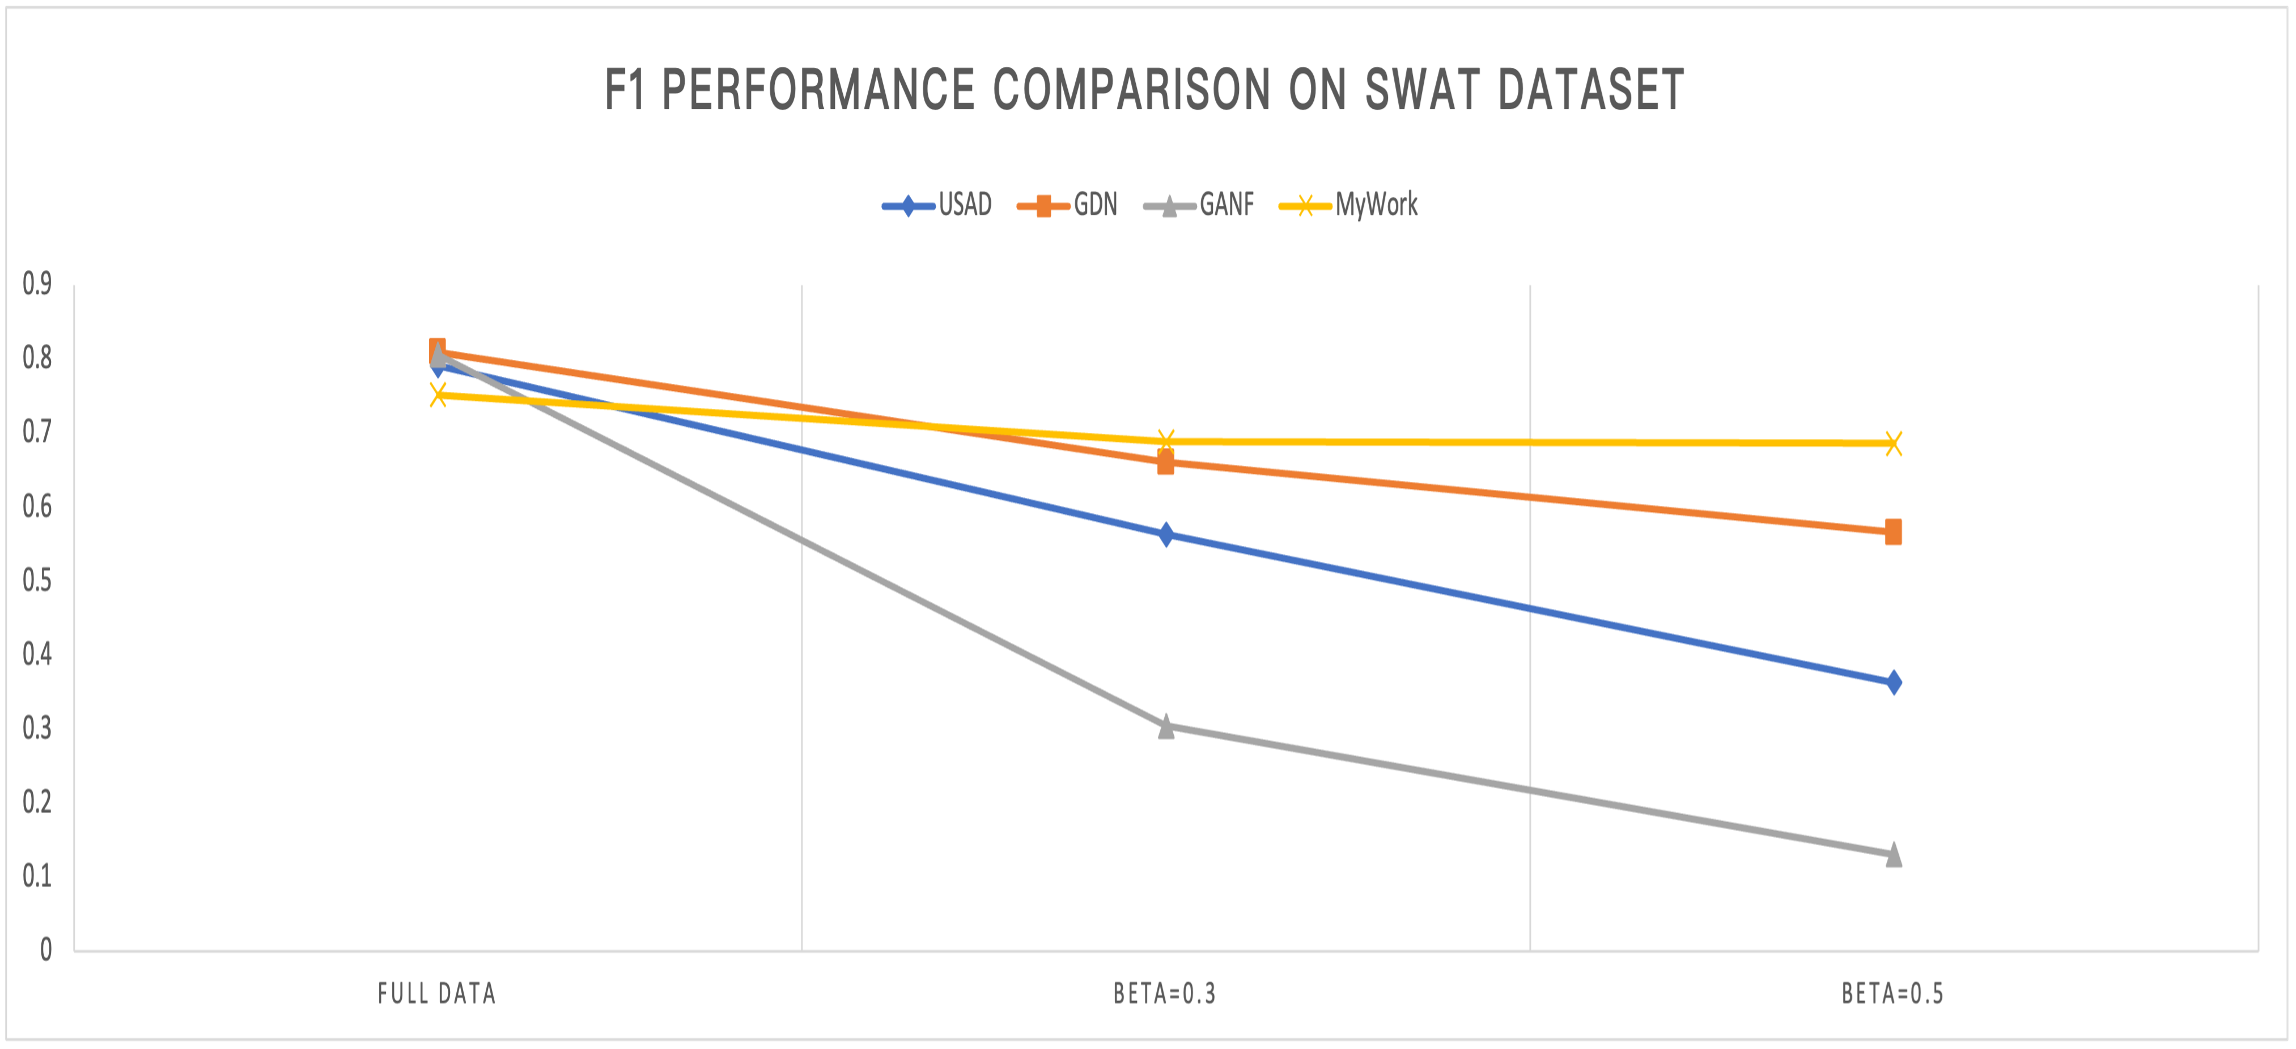
\includegraphics[width = 0.8\textwidth]{chapter4/swat-compare.png}
  \caption{所有方法在SWAT数据集上的性能比较}
  \end{figure}

图4-1展示了SWaT 数据集中对比结果,其中横坐标代表缺失值场景,纵坐标代表F1综合性能分数。可以看到我们在完整数据集下的性能接近当前的SOTA方案,在30\%缺失值的情况下
对比SOTA方案提升约为120\%至4\%,在在50\%缺失值的情况下对比SOTA方案提升约为522\%至20\%。

\begin{figure}[htb]
  \centering
  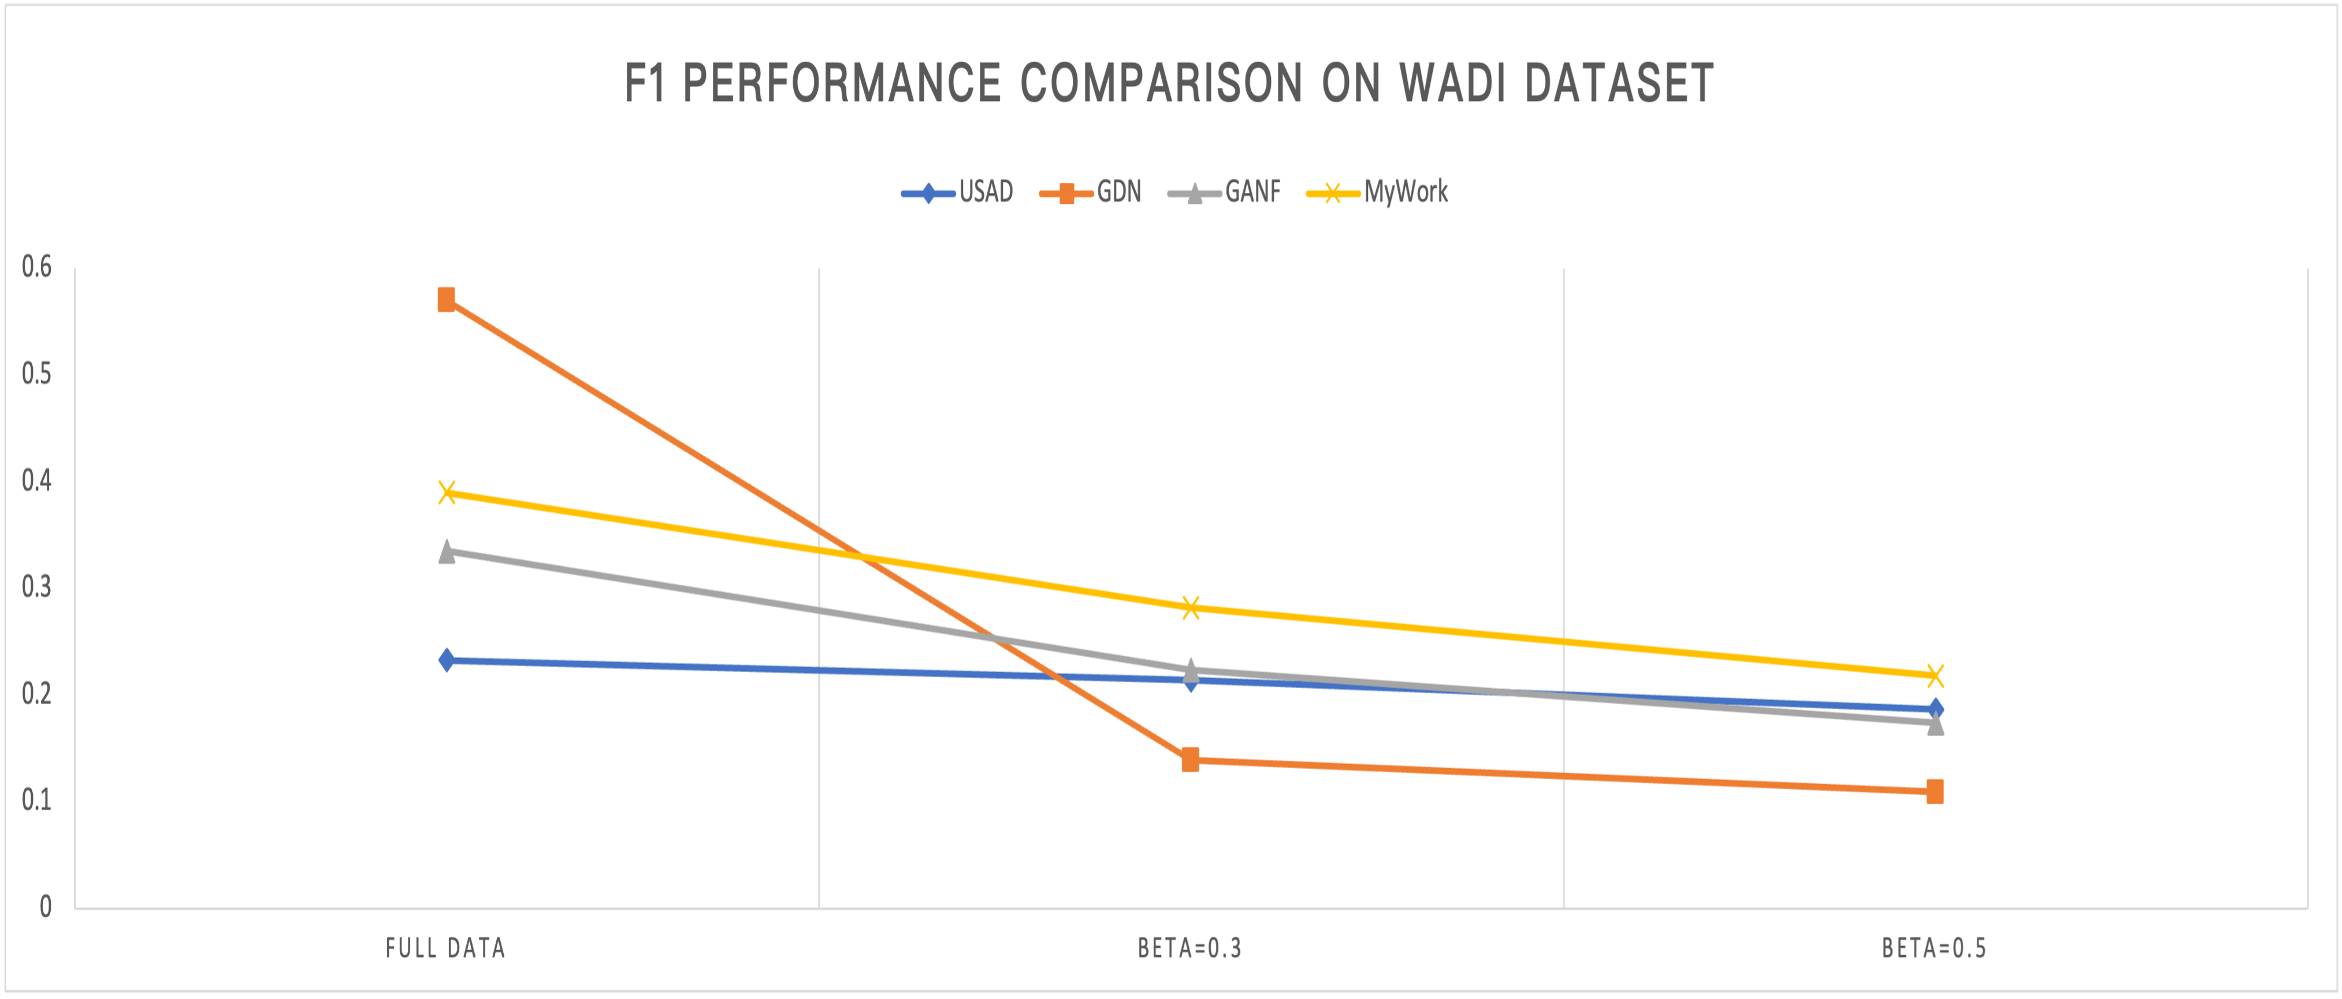
\includegraphics[width = 0.8\textwidth]{chapter4/wadi-compare.png}
  \caption{所有方法在WADI数据集上的性能比较}
  \end{figure}

图4-2展示了WADI 数据集中对比结果,其中横坐标代表缺失值场景,纵坐标代表F1综合性能分数。可以看到我们在完整数据集下的性能接近当前的SOTA方案,在30\%缺失值的情况下
对比SOTA方案提升约为103\%至26\%,在在50\%缺失值的情况下对比SOTA方案提升约为99\%至25\%。

\begin{figure}[htb]
  \centering
  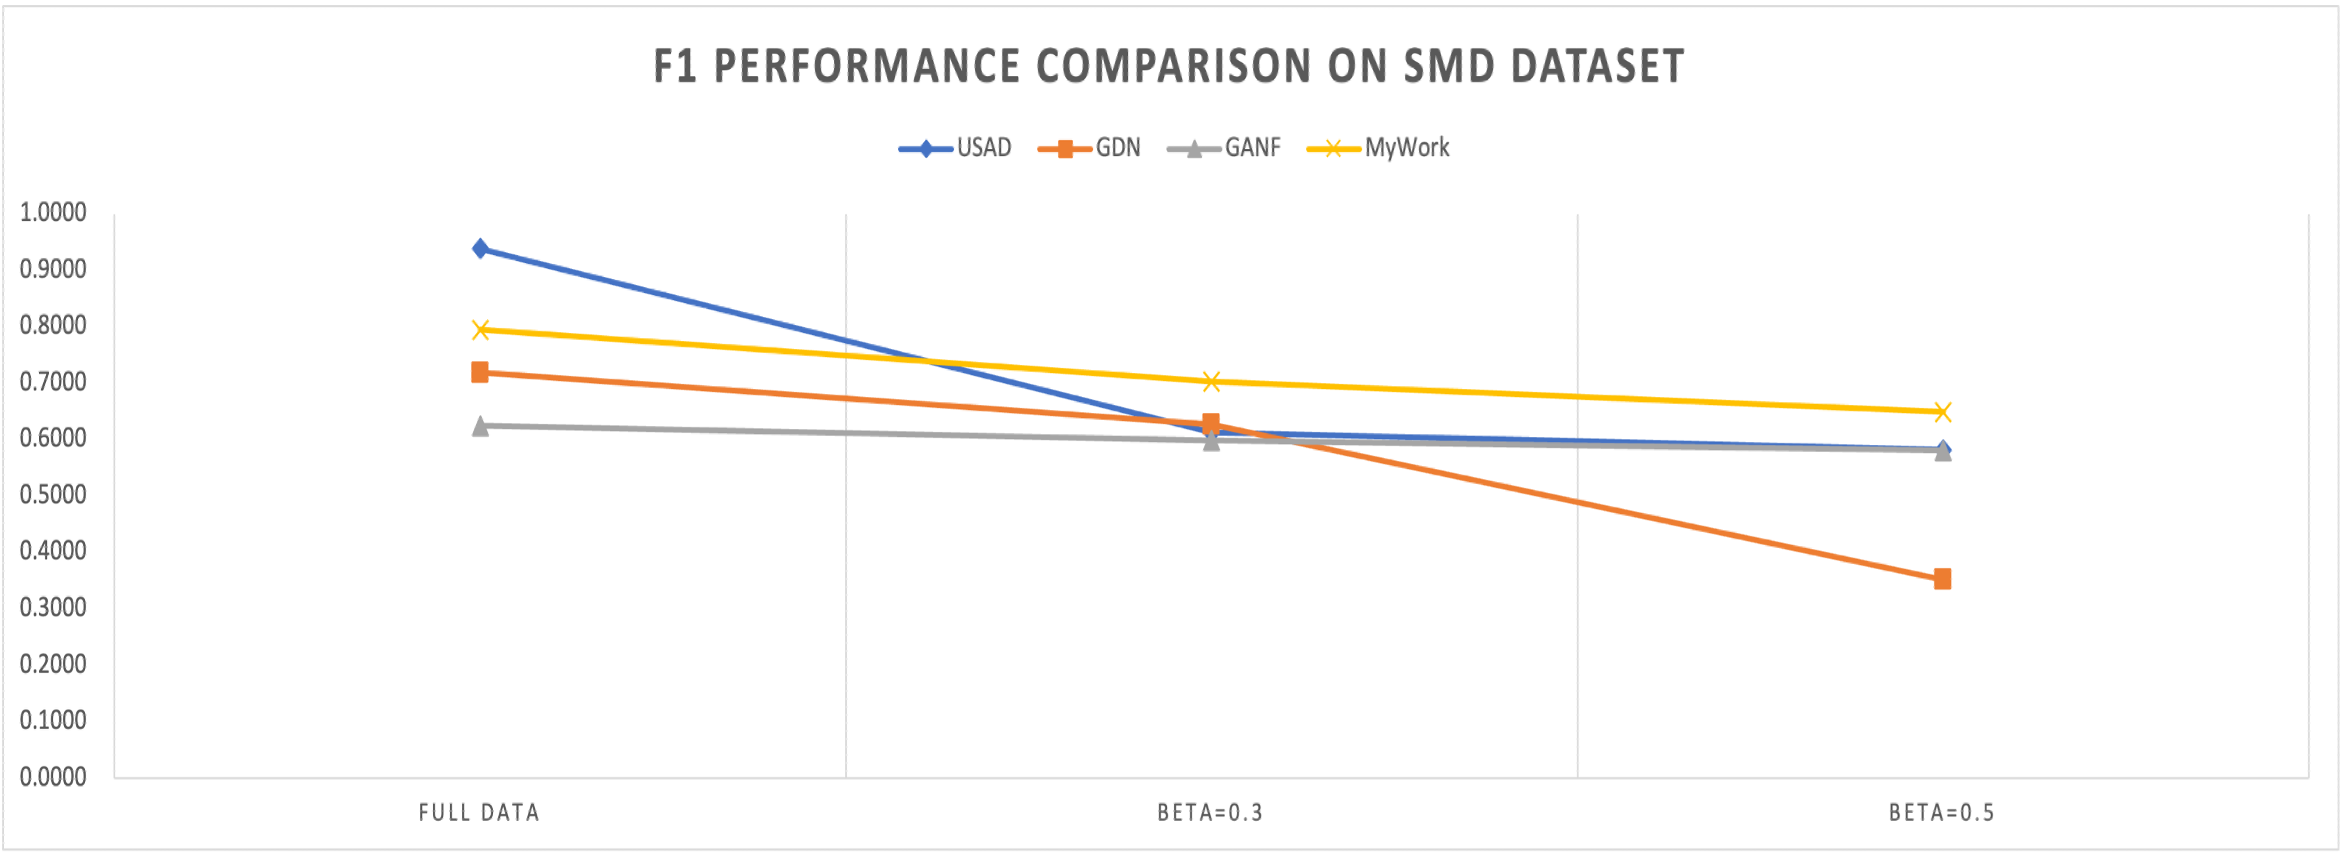
\includegraphics[width = 0.8\textwidth]{chapter4/smd-comapre.png}
  \caption{所有方法在SMD数据集上的性能比较}
  \end{figure}
图4-3展示了SMD 数据集中对比结果,其中横坐标代表缺失值场景,纵坐标代表F1综合性能分数。可以看到我们在完整数据集下的性能接近当前的SOTA方案,在30\%缺失值的情况下
对比SOTA方案提升约为17\%至12\%,在在50\%缺失值的情况下对比SOTA方案提升约为84\%至11\%。


常见的缺失值填充方法有填充默认值、均值、众数、KNN填充等。其中填充固定值选取某个固定值/默认值填充缺失值。其中对每一列的缺失值,填充当列的均值。填充均值得是对每一列的缺失值,
填充当列的中位数。填充众数指的是对每一列的缺失值,填充当列的众数。填充上下条的数据指的是对每一条数据的缺失值,填充其上下条数据的值。
由于传统多元时间序列异常检测模型只能在不包含缺失值的数据集上执行异常检测任务,因此在对比传统多元时间序列异常检测模型在包含缺失值的数据集上的性能表现时必须要
先对缺失值进行填充。需要注意的是,对于异常检测任务,我们只能使用检测时刻之前的历史数据进行填充而不能使用检测时刻之后的未来数据进行填充。在此条件的限制下,
我们为每个对比方法先验得在sklearn提供的经典数据填充方法(均值填充,中位数填充,常数填充,众数填充)中选择效果最好的填充方法,最终对比方法为 
USAD+Mean, GDN+Mean, GANF+Median。

如表4-4, 表4-5, 表4-6所示,我们测试了不同程度下删除数据后模型性能表现。通过实验结果我们可以看到,我们在SOTA模型的原场景下接近SOTA的性能,
同时在我们设计的新的场景下超过SOTA模型的表现,以此可以证明我们的模型在缺失值场景下具有较好的性能表现。
同时我们的模型在beta = 0 至 beta = 0.3 与 beta = 0.3 至 beta = 0.5 的场景变换中,性能下降最低,这证明了我们的模型在数据损失的情况下性能
下降最不明显,对数据缺失具有鲁棒性。

\begin{table}[htb]
  \caption{填充数据集后所有方法在SWAT数据集上的性能比较}
  %\label{comparison_results}
  \small
  \centering
  \setlength{\tabcolsep}{0.8mm}{
  \begin{tabular}{lccccccccc}\toprule
  Method & \multicolumn{3}{c}{SMD FULL DATA} & \multicolumn{3}{c}{SMD DROP 0.3 DATA} & \multicolumn{3}{c}{SMD DROP 0.5 DATA} \\ \cmidrule(r){2-4} \cmidrule(r){5-7} \cmidrule(r){8-10}
      & F1-Score & Precision & Recall & F1-Score & Precision & Recall & F1-Score & Precision & Recall\\ \midrule
      USAD+Mean & 0.7917 & 0.9851 & 0.6618 & 0.59172 & 0.44499 & 0.88284 & 0.3818 & 0.25788 & 0.735315 \\
      GDN+Mean & 0.8100 & 0.9935 & 0.6812 & 0.69393 & 0.857535 & 0.58275 & 0.5948 & 0.763455 & 0.487305 \\
      GANF+Median & 0.8065 & 0.9892 & 0.6808 & 0.31996 & 0.212625 & 0.64617 & 0.1379 & 0.073815 & 1 \\
      MMTSAD & 0.7522 & 0.9583 & 0.6191 & 0.6886 & 0.8106 & 0.5986 & 0.6869 & 0.784 & 0.6112 \\
%\bfseries MUSE-Net& \bfseries 2.89 & \bfseries 1.10 & \bfseries 2.74 & \bfseries 1.05 & \bfseries 15.47 & \bfseries 5.47 & \bfseries 14.45 & \bfseries 5.54 & \bfseries 17.19 \\
\bottomrule
\centering
\end{tabular}}
\end{table}

\begin{table}[htb]
  \caption{填充数据集后所有方法在WADI数据集上的性能比较}
  %\label{comparison_results}
  \small
  \centering
  \setlength{\tabcolsep}{0.8mm}{
  \begin{tabular}{lccccccccc}\toprule
  Method & \multicolumn{3}{c}{SMD FULL DATA} & \multicolumn{3}{c}{SMD DROP 0.3 DATA} & \multicolumn{3}{c}{SMD DROP 0.5 DATA} \\ \cmidrule(r){2-4} \cmidrule(r){5-7} \cmidrule(r){8-10}
      & F1-Score & Precision & Recall & F1-Score & Precision & Recall & F1-Score & Precision & Recall\\ \midrule
      USAD+Mean & 0.2328 & 0.9947 & 0.1318&  0.2243 & 0.267855 & 0.19299 & 0.1959&  0.19918 & 0.19278 \\
      GDN+Mean & 0.5700 & 0.9750 & 0.4019 & 0.1458 & 0.08421 & 0.543585 & 0.2067 & 0.11466 & 1 \\
      GANF+Mean & 0.3348 & 0.2040 & 0.9324 & 0.2345 & 0.14658 & 0.58632 & 0.1826&  0.175035&  0.19089 \\
      MMTSAD & 0.3897 & 0.2718 & 0.6883 & 0.2821 & 0.2102 & 0.4286  & 0.2179 & 0.2179 & 0.5844 \\
%\bfseries MUSE-Net& \bfseries 2.89 & \bfseries 1.10 & \bfseries 2.74 & \bfseries 1.05 & \bfseries 15.47 & \bfseries 5.47 & \bfseries 14.45 & \bfseries 5.54 & \bfseries 17.19 \\
\bottomrule
\centering
\end{tabular}}
\end{table}

\begin{table}[htb]
  \caption{填充数据集后所有方法在SMD数据集上的性能比较}
  %\label{comparison_results}
  \small
  \centering
  \setlength{\tabcolsep}{0.8mm}{
  \begin{tabular}{lccccccccc}\toprule
  Method & \multicolumn{3}{c}{SMD FULL DATA} & \multicolumn{3}{c}{SMD DROP 0.3 DATA} & \multicolumn{3}{c}{SMD DROP 0.5 DATA} \\ \cmidrule(r){2-4} \cmidrule(r){5-7} \cmidrule(r){8-10}
      & F1-Score & Precision & Recall & F1-Score & Precision & Recall & F1-Score & Precision & Recall\\ \midrule
      USAD+Mean & 0.9382 & 0.9314 & 0.9617 & 0.6435 & 0.494865 & 0.92001 & 0.6109 & 0.46116 & 0.904785 \\
      GDN+Mean & 0.7183 & 0.7079 & 0.7294 & 0.6577 & 0.625275 & 0.693735 & 0.3693 & 0.24822 & 0.721455 \\
      GANF+Median & 0.6241 & 0.5131 & 0.7963 & 0.6282 & 0.501795 & 0.84 & 0.6098 & 0.445935 & 0.964425 \\
      MMTSAD & 0.7949 & 0.9051 & 0.7086 & 0.7025 & 0.7367 & 0.6714& 0.6491 & 0.5881 & 0.7243 \\
%\bfseries MUSE-Net& \bfseries 2.89 & \bfseries 1.10 & \bfseries 2.74 & \bfseries 1.05 & \bfseries 15.47 & \bfseries 5.47 & \bfseries 14.45 & \bfseries 5.54 & \bfseries 17.19 \\
\bottomrule
\centering
\end{tabular}}
\end{table}

我们通过设置以下三种情况来验证模型各个模块的有效性,即:
\begin{enumerate}
  \item Full model: 不修改模型
  \item Drop MMAR: 删除时间位置编码模块以及掩码注意力表征模块
  \item Drop CNF-AD: 用一个简单的全连接层决策(正常/异常)结果
\end{enumerate}

如表所示,我们在缺失值为0.3的SWAT数据集和缺失值为0.5的SWAT数据集上进行了消融实验,实验结果表明删除时间位置编码模块以及掩码注意力表征模块后的模型(Drop MMAR)在两种场景下相比较完整的模型性能
分别下降了27\%和49\%;删除CNF-AD模块后的模型在两种场景下性能下降分别为(34\%和38\%)。

通过消融实验我们得到了以下结果:Drop MMAR 性能下降,证明了MMAR能够有效表征缺失值多元时间序列,Drop MMAR 性能下降率 与 数据确实率成正比,证明了MMAR对不同缺失值场景下具有鲁棒性, Drop CNF-AD 性能下降,证明了 CNF-AD能够有效识别异常。

\begin{table}[ht]
  \caption{消融实验性能比较}
  %\label{comparison_results}
  \small
  \centering
  \setlength{\tabcolsep}{0.8mm}{
  \begin{tabular}{lcccccc}\toprule
  Method & \multicolumn{3}{c}{SWAT DROP 0.3 DATA} & \multicolumn{3}{c}{SWAT DROP 0.5 DATA}  \\ \cmidrule(r){2-4} \cmidrule(r){5-7} 
      & F1-Score & Precision & Recall & F1-Score & Precision & Recall \\ \midrule
      full model & 0.6886 & 0.8106 & 0.5986  & 0.6869 & 0.784 & 0.6112 \\
      drop MMAR & 0.5734 (-27\%) & 0.6282 & 0.6036  & 0.3405(-49\%) & 0.2117  & 0.8706 \\ 
      drop CNF-AD & 0.4578(-34\%) & 0.3207 & 0.7996  & 0.4958 (-38\%)&  0.4933 &  0.6133\\       
%\bfseries MUSE-Net& \bfseries 2.89 & \bfseries 1.10 & \bfseries 2.74 & \bfseries 1.05 & \bfseries 15.47 & \bfseries 5.47 & \bfseries 14.45 & \bfseries 5.54 & \bfseries 17.19 \\
\bottomrule
\centering
\end{tabular}}
\end{table}

\section{本章小节}[Introduction]
本文针对工业场景中更加常见的含缺失值时间序列异常检测任务,提出一种基于注意力重新表征的时间序列异常检测算法。该算法首先将包含缺失值的时间序列数据通过时间位置编码对时间序列中不同时间戳关联性进行建模;然后通过掩码注意力表征模块学习不同时间戳之间数据的关联关系并表征为一个高维的嵌入式编码矩阵;最后引入条件标准化流对数据进行重建,以重建概率作为数据异常评分。最后本章做了两部分实验,其中第一部分为性能实验,对比MMTSAD与当前多元时间序列异常检测SOTA在三种缺失值场景下的性能表现;第二部分为消融实验,分析不同模块在完成异常检测任务过程的效果。
% \chapter{初生对流检测系统的设计与实现}[Example]

\section{引言}[Number]
本章节设计并实现了一个对流初生检测的系统。此系统集成了前文章节中
所提及的对流初生检测算法模型,同时包括卫星原始数据的处理到对流检测的端到端处理过程。本章节将从
系统后端架构,系统任务计算模块和系统可视化模块三个部分展开。
\section{系统设计架构}
本文的系统采用的是前后端分离技术,B/S的设计架构,后端采用的是Flask的HTTP服务器,由Python
语言支持,前端是HTML、CSS、JavaScript编写的前端页面。运行方式为配置如表
~\ref{tab:env3}~内所示环境后,解压文件夹,命令行执行Run.sh。

\begin{table}[h]
	\renewcommand{\arraystretch}{1.3}
	\caption{系统运行环境}
	\label{tab:env3}
	\vspace{0.5em}\centering\wuhao
	\begin{tabular}{c c}
		\toprule[1.5pt] 环境参数 & 配置 \\
		\midrule[1pt] 
		系统环境 & Ubuntu/CentOs/RetHat \\
		软件环境 & tensorflow1.13.0、pytorch1.0.1、Anaconda3 \\
        硬件环境 & 内存1GB、显存1GB \\ 
		编程语言 & Python、HTML、CSS、JavaScript \\
		\bottomrule[1.5pt]
	\end{tabular}
\end{table}

本系统的后端为单任务流模式,
每当用户上传一个卫星云图数据文件,自动启动开启一个初生对流检测的执行,
由于卫星云图下存在很多个像素点,模型在执行过程中采用的是每个像素点周围的15$\times$15像元作为样本,
因此提取完像素后由系统自动判识并开启多进程执行该检测模型,
并将进度实时显示到前端的页面上,当所有像素点都判识完成,并完成结果合并成结果图,此时执行完成。

\section{检测执行模块设计}
此部分主要实现如何端到端的实现卫星云图的处理到对流初生检测过程。
本系统的综合架构如图~\ref{fig:system1}~所示。
此阶段依赖于用户对于检测上传的参数表达,检测上传包含卫星数据地址、模型选择以及执行模式等。
首先是卫星云图序列的处理,首先用户在上传任务之后,系统自动根据用户上传目录的卫星云图序列判断未检测的
数量,并将其添加到检测队列中。初生对流检测数据的处理则涉及到将提取多通道的卫星红外云图,以及利用
当前阈值法对其进行规则处理。此时如果采取的是多进程的执行模式,
检测执行模块会自动开启多进程执行,但是相应占用的系统资源也会增加。模型选择则是每次执行初生对流检测所采取的模型。

\begin{figure}[h]
	\centering
	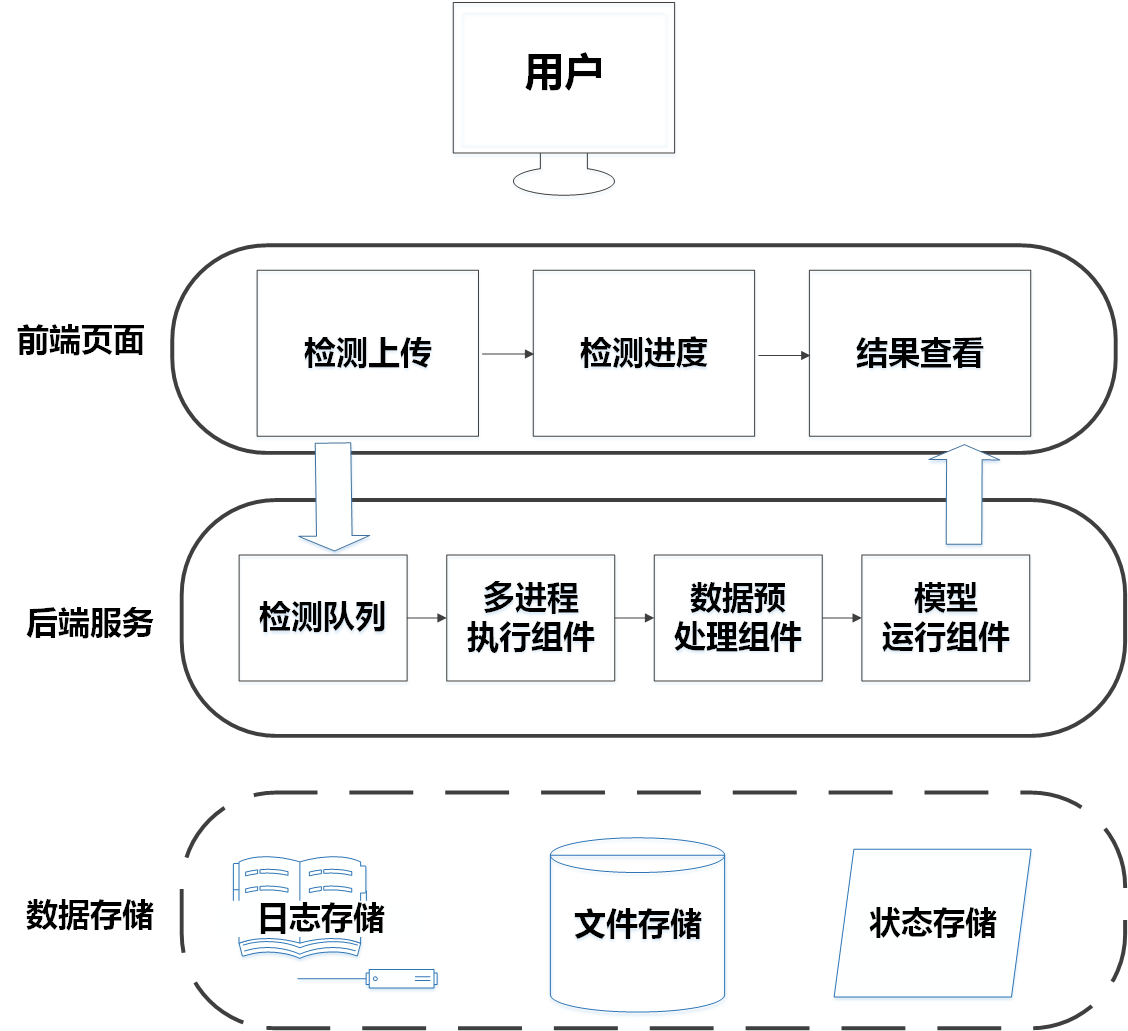
\includegraphics[width = 0.6\textwidth]{系统模块.png}
	\caption{系统综合架构}
	\label{fig:system1}
\end{figure}

同时系统还有错误检测和恢复的功能,如图~\ref{fig:err}~所示。
系统错误恢复是指系统执行过程中如果出现其他中断,例如断电、宕机等问题,
如果磁盘没有损坏则能够对检测进度进行恢复;错误检测则是如果存在例如时序不全或者卫星云图损坏等
错误,会自动检测而不是崩溃影响后续任务的执行进度。

\begin{figure}[h]
	\centering
	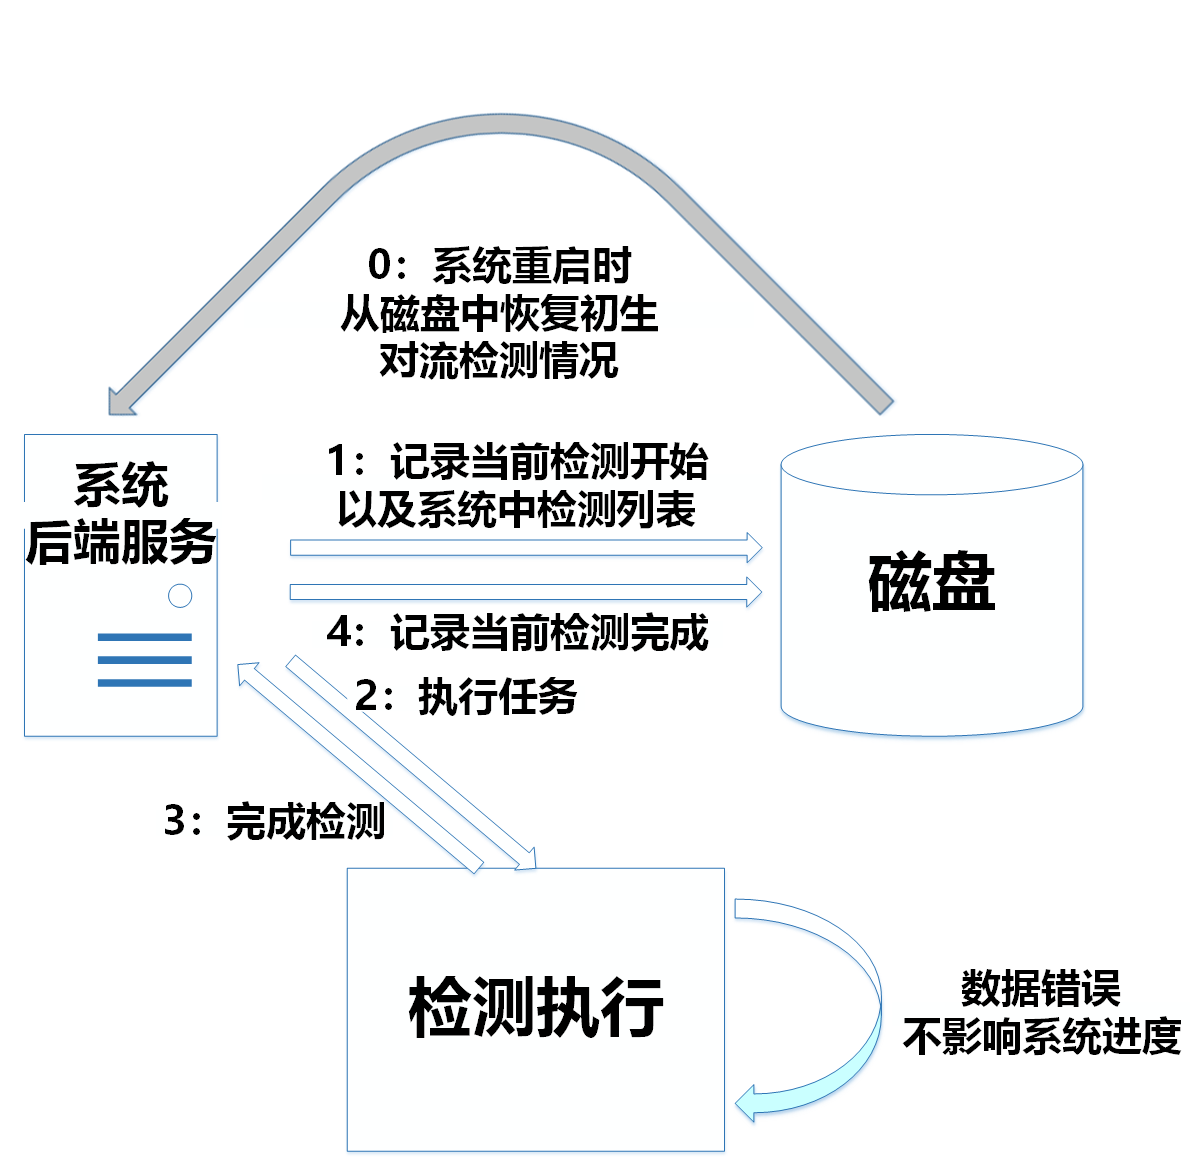
\includegraphics[width = 0.6\textwidth]{纠错模块.png}
	\caption{系统错误检测及恢复模块}
	\label{fig:err}
\end{figure}

\section{系统的可视化页面设计}
系统启动方式为在服务器运行脚本run.sh,启动后可通过主机地址加端口号(ip:port)的方式访问。
系统访问默认进入对流初生检测系统的可视化主界面,如图~\ref{fig:sys-main}~所示,主界面左侧有快捷访问的菜单栏。
可通过访问不同快捷菜单进入不同的系统界面。菜单栏中主界面为系统启动的默认界面同时具有查看检测进度的功能,
查看完成任务可查看历史检测结果,
任务上传负责上传检测任务,文件管理可直接以文件的形式查看检测数据。
\begin{figure}[h]
	\centering
	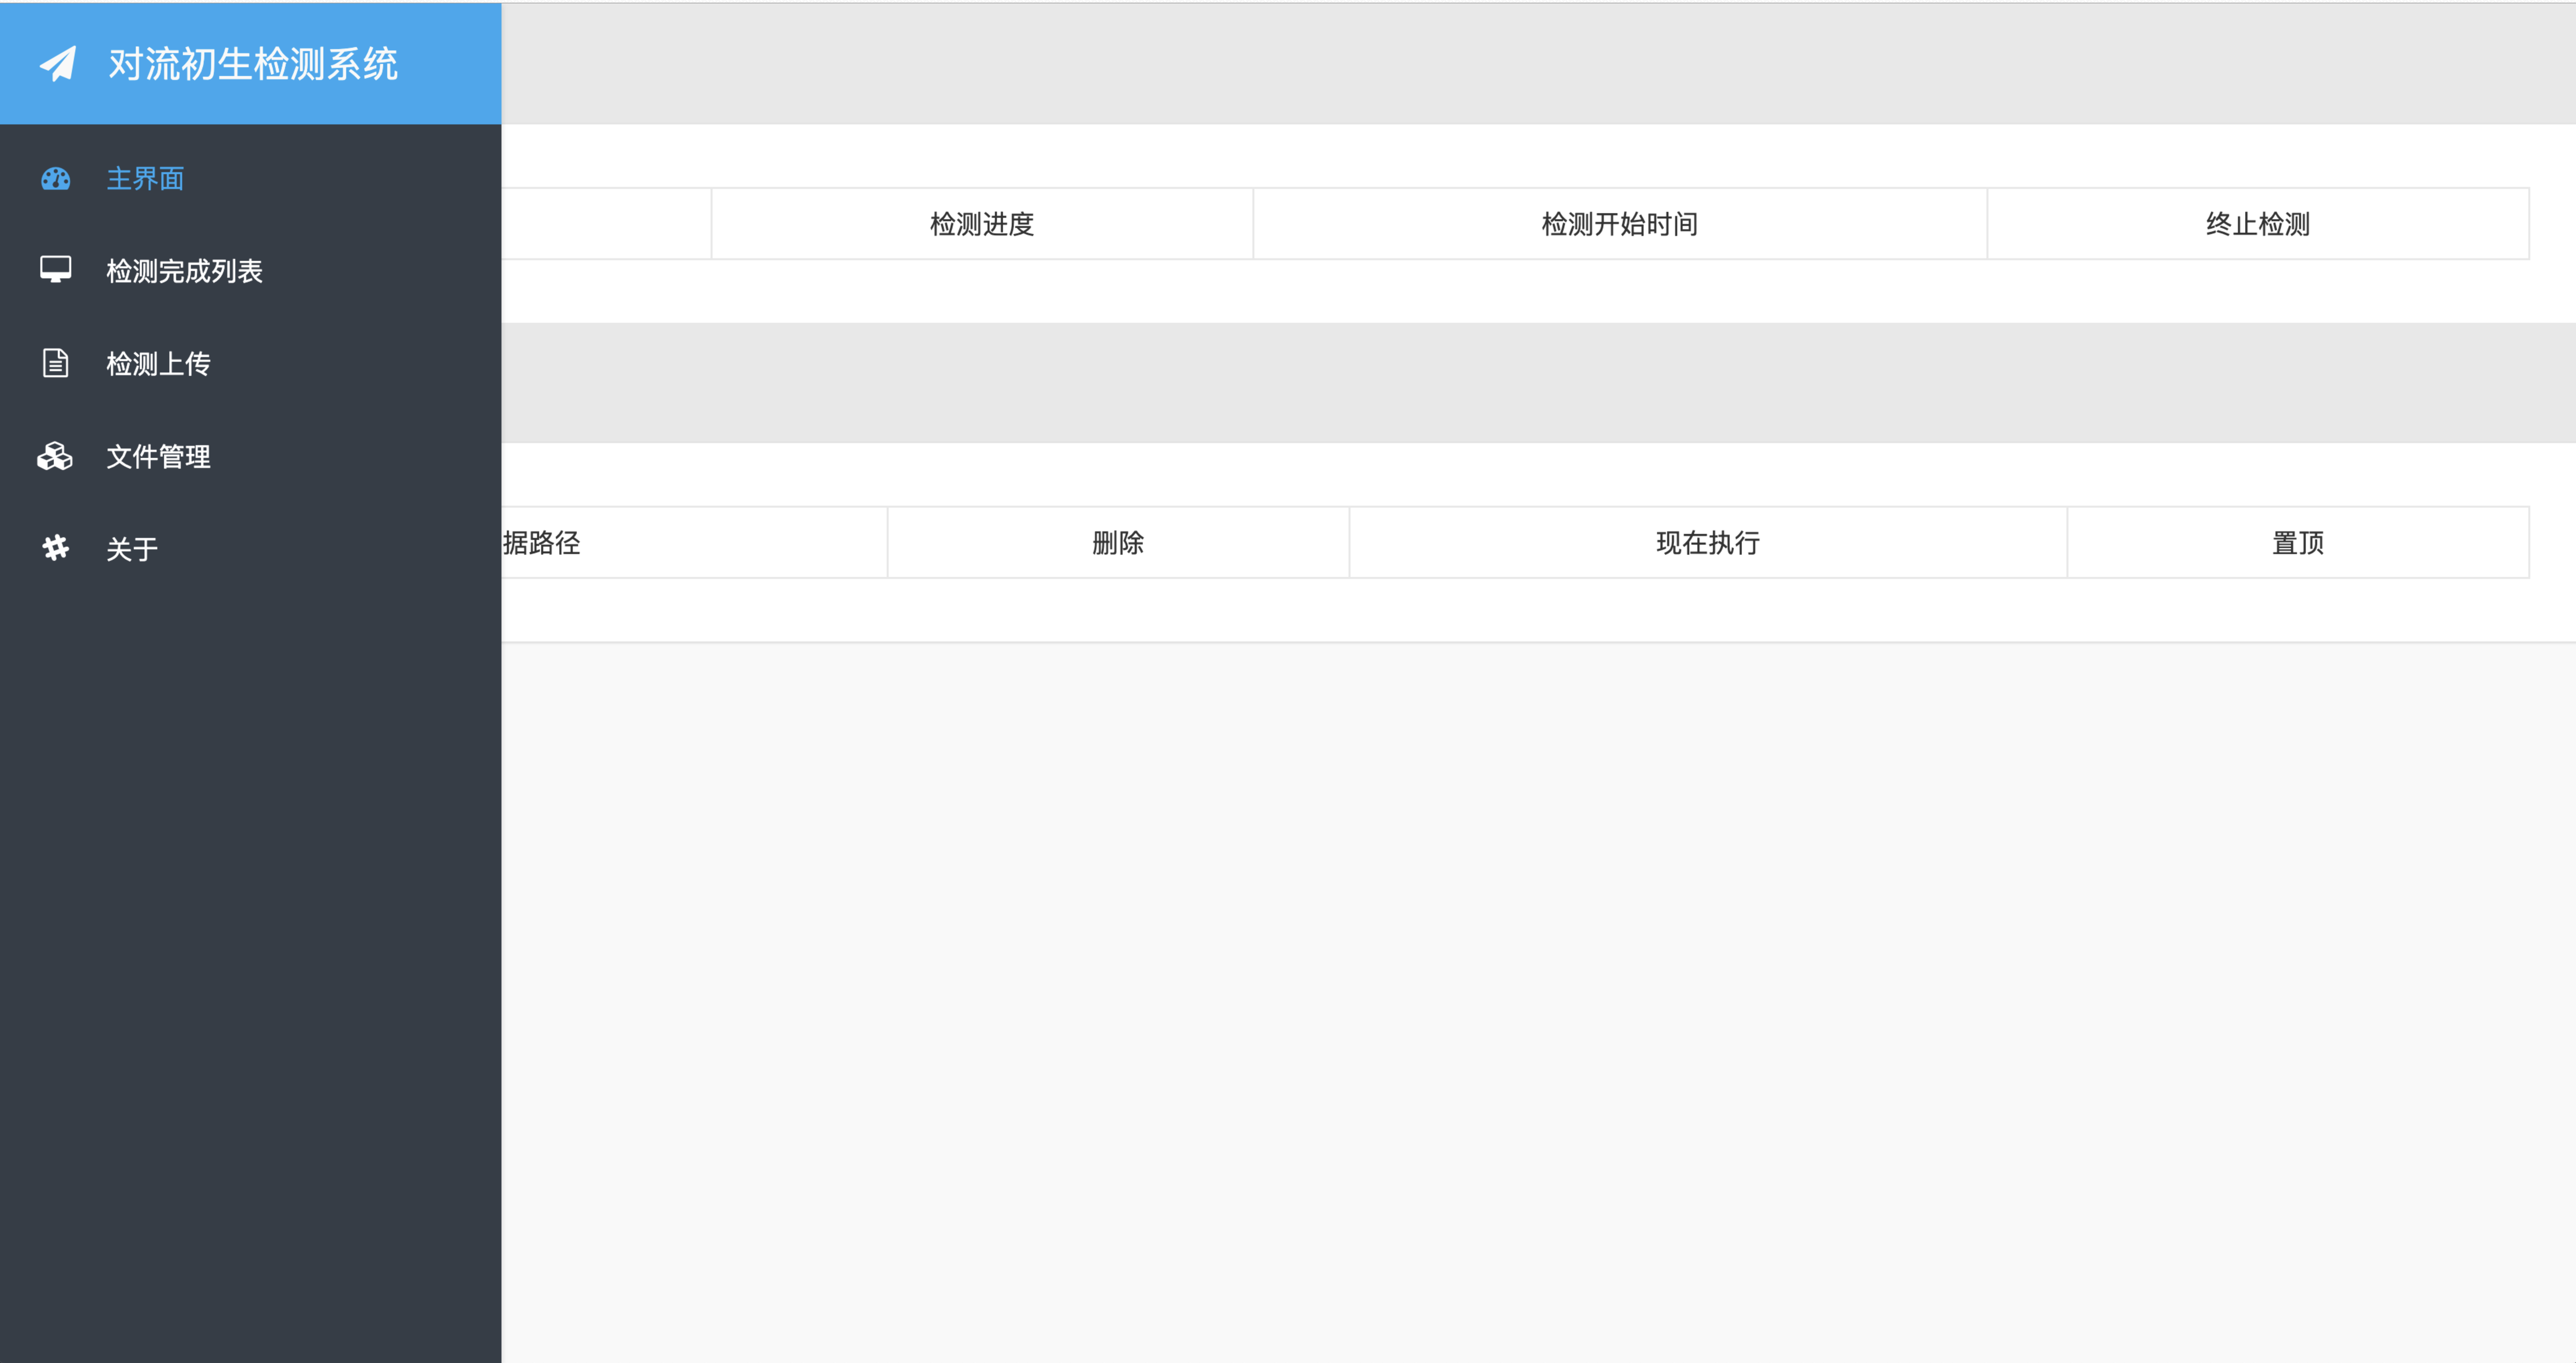
\includegraphics[width = 0.8\textwidth]{主界面2.png}
	\caption{系统默认界面及菜单栏}
	\label{fig:sys-main}
\end{figure}

\subsection{检测上传界面}
检测上传界面依次有任务目录,模型选择以及执行模式三个选项。
如果检测上传成功则会跳转至进度界面,
如果检测上传失败(例如目录不存在,模型不存在等)则会有弹窗提醒检测上传失败。
通常情况下检测上传的流程为先获取检测数据路径,以路径名作为任务名输入,可利用系统中的
文件管理可以获取到数据路径,其中的卫星数据按照日期由
新到旧排序,如图~\ref{fig:sys-getpath}~所示。
\begin{figure}[h]
	\centering
	\includegraphics[width = 0.8\textwidth]{获取路径2.png}
	\caption{文件管理界面获取路径}
	\label{fig:sys-getpath}
\end{figure}

之后进入检测上传界面输入路径,执行模式以及模型选择,如图~\ref{fig:sys-missupload}~所示。执行模式为1时会立即执行该任务,无需进入等待列表等待。
模型默认为本文的基准线模型Dense-S-RCNN,也可以采用其他模型进行预测。
\begin{figure}[h]
	\centering
	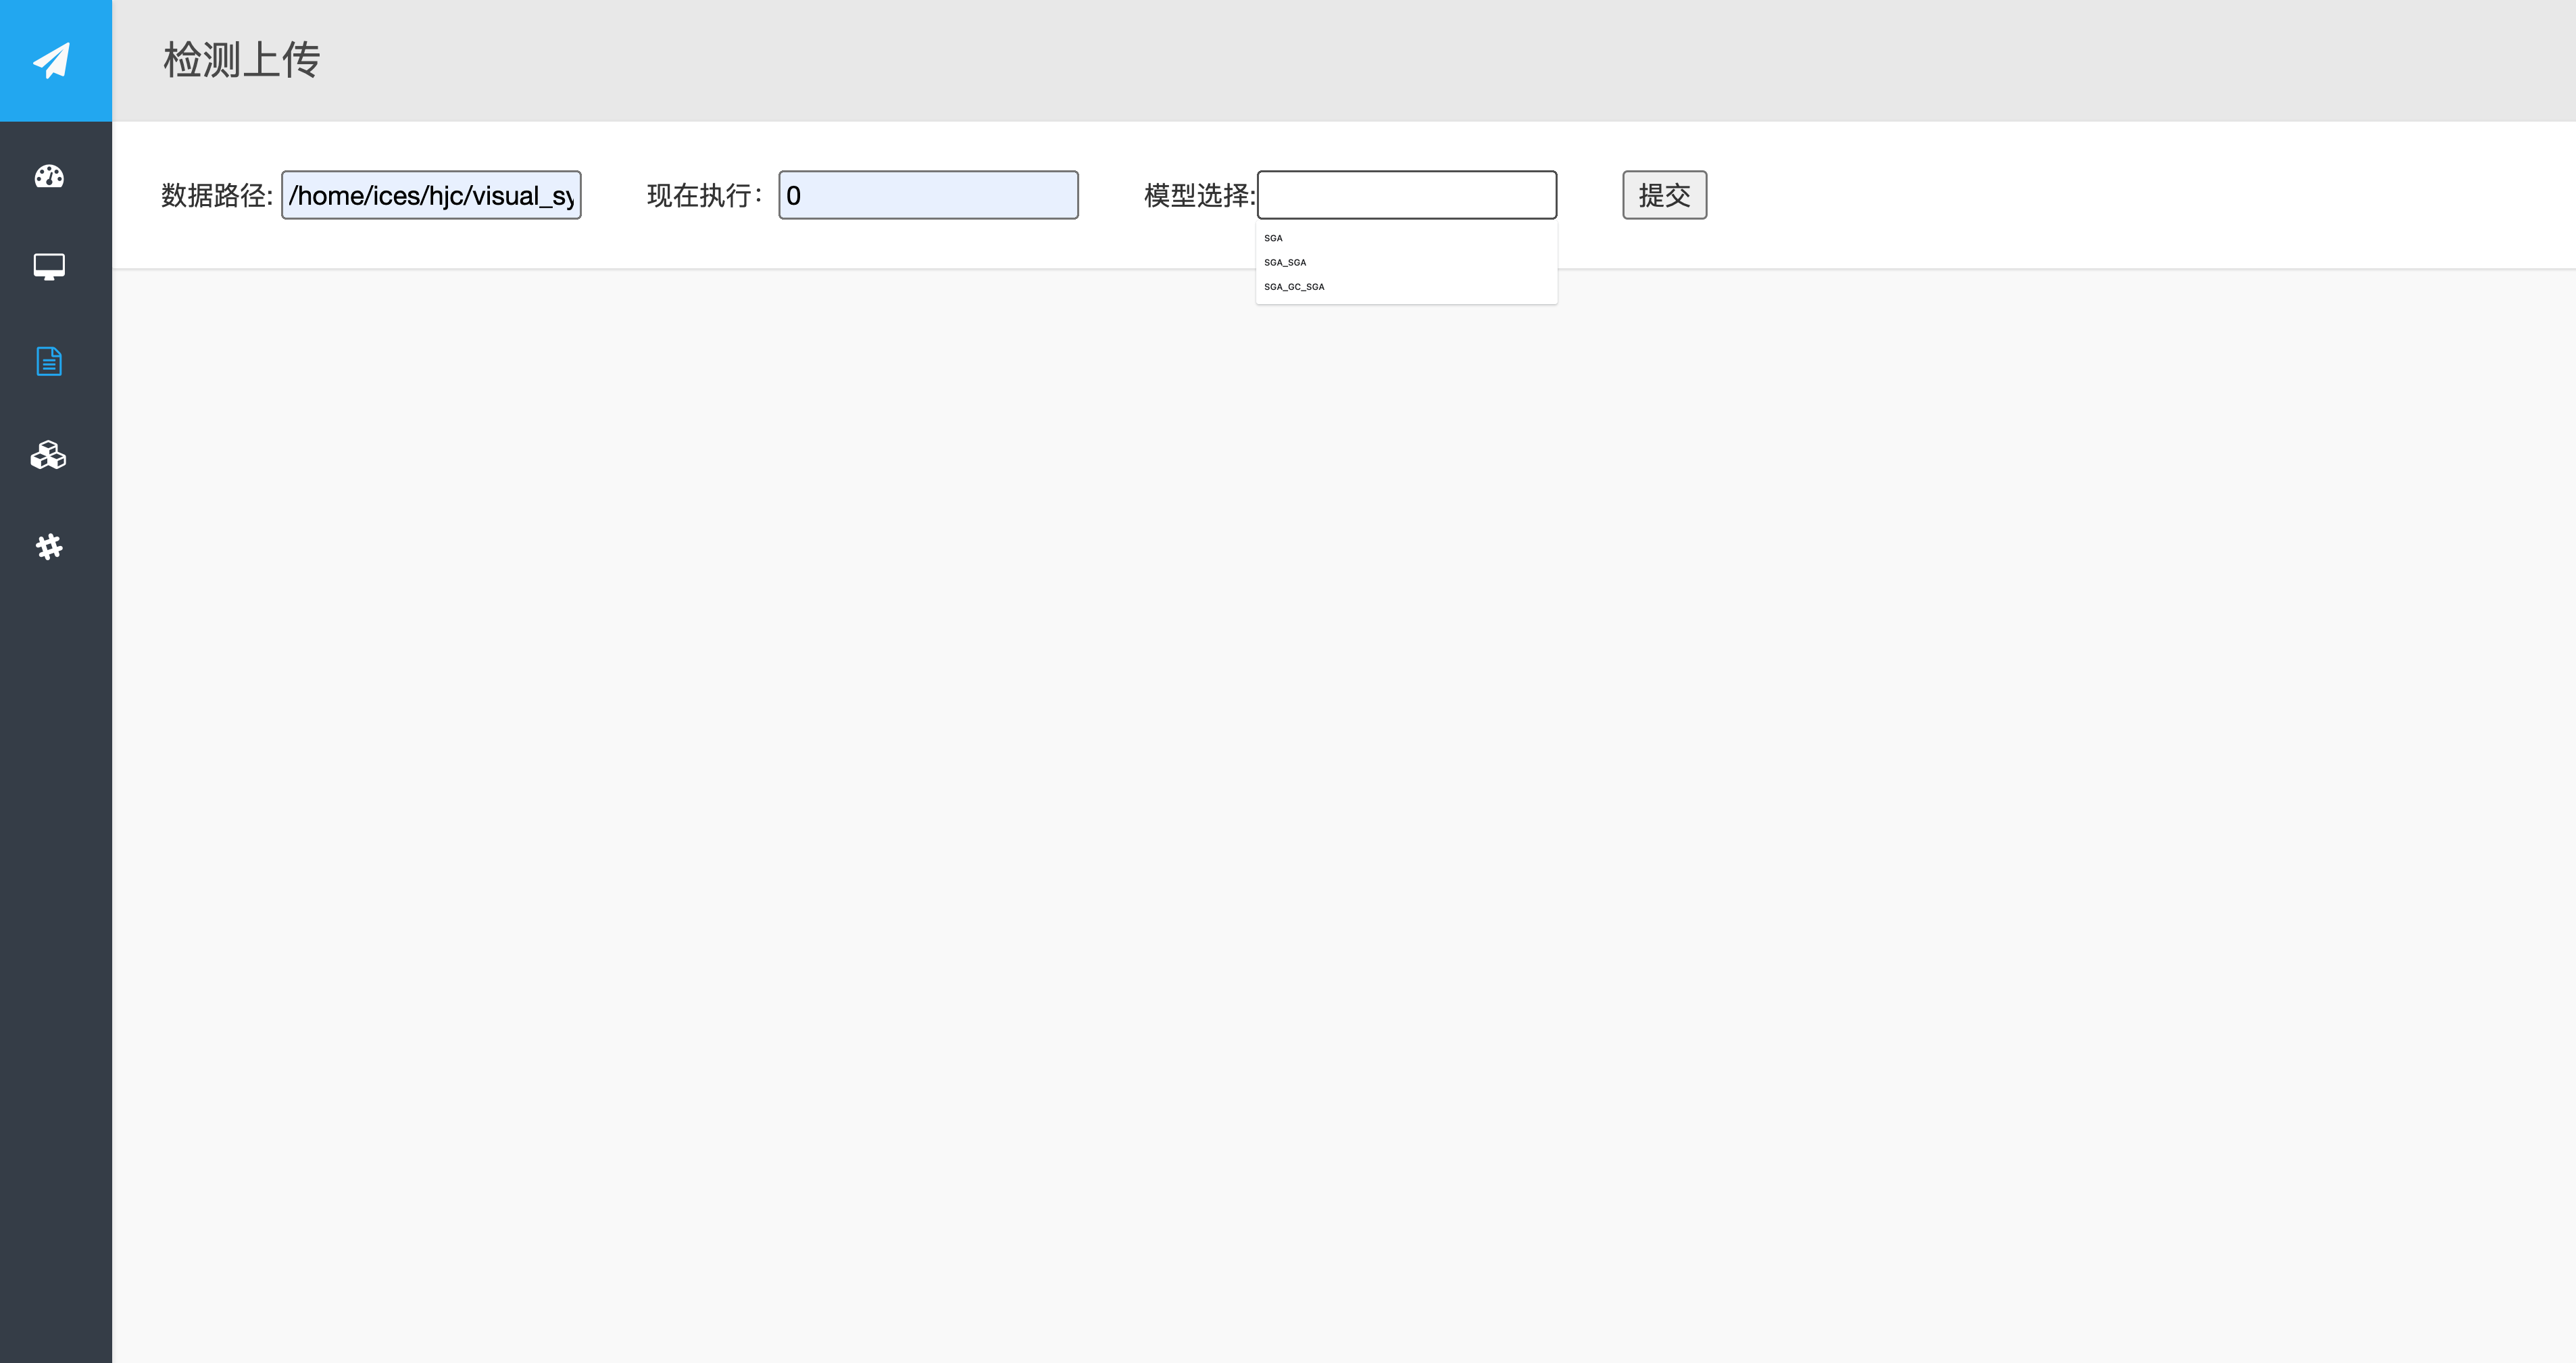
\includegraphics[width = 0.8\textwidth]{检测上传2.png}
	\caption{检测上传界面}
	\label{fig:sys-missupload}
\end{figure}

\subsection{检测进度界面}
此界面为检测的进度页面,如图~\ref{fig:sys-missjd}~所示,其中执行中的检测进度采用了ajax技术定时访问后端状态,从而实时显示到前端。
检测进度界面中在等待中的检测会按照排序
排队等待,用户也可以手动拖拽以调整其次序。如果用户选择终止程序,可以选择终止执行中的检测
。用户如果想直接执行后续等待中的检测,也可以选择立即执行,此时会有弹窗提醒,
如果选择否则无事发生,选择是则会中断执行中任务,立即执行等待中的检测。被中断的检测也会
排序在等待中检测的第一位。同时用户也可选择删除检测,此时会将等待中的检测删除。
\begin{figure}[h]
	\centering
	\includegraphics[width = 0.8\textwidth]{检测进度2.png}
	\caption{检测进度界面}
	\label{fig:sys-missjd}
\end{figure}

检测结束后,可通过查看检测完成列表来查看检测情况,如图~\ref{fig:sys-missdone}~所示,通常情况检测状态为完成(done),存在
一些情况会导致检测失败,比如数据长度不足或者模型不存在等,检测失败的情况不会影响后续数据的检测
进度。
\begin{figure}[h]
	\centering
	\includegraphics[width = 0.8\textwidth]{检测完成2.png}
	\caption{检测完成列表界面}
	\label{fig:sys-missdone}
\end{figure}

\subsection{结果预览界面}
检测执行完成后,会将数据输出结果重新输出到源数据文件夹下面,用户可以通过结果预览界面
查看检测结果文件是否正确输出出来。如图~\ref{fig:sys-1}~\ref{fig:sys-2}~\ref{fig:vis-ans}~所示。
\begin{figure}[h]
	\centering
	\includegraphics[width = 0.8\textwidth]{系统12.png}
	\caption{不同模型结果预览界面}
	\label{fig:sys-1}
\end{figure}

\begin{figure}[h]
	\centering
	\includegraphics[width = 0.8\textwidth]{系统22.png}
	\caption{模型输出结果预览界面}
	\label{fig:sys-2}
\end{figure}

\begin{figure}[h]
	\centering
	\subfigure[结果预览1]{
		\begin{minipage}[t]{0.4\linewidth}
			\centering
			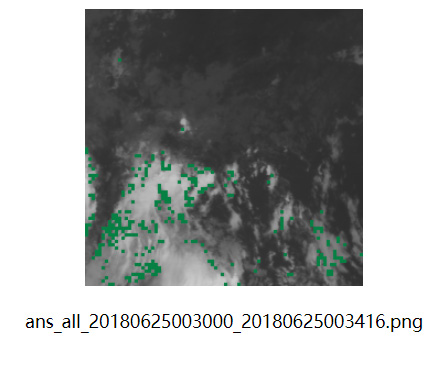
\includegraphics[width = 2.2in]{结果1.jpg}
		\end{minipage}
	}
	\subfigure[结果预览2]{
		\begin{minipage}[t]{0.4\linewidth}
			\centering
			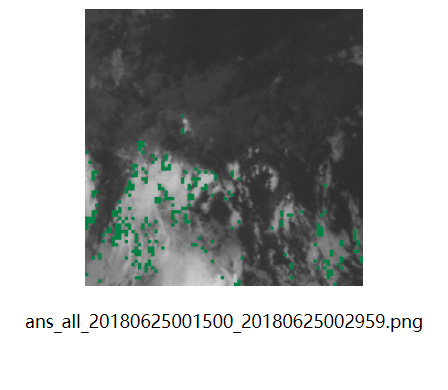
\includegraphics[width = 2.2in]{结果2.jpg}
		\end{minipage}
	}
	\caption{可视化模型运行结果图}
	\label{fig:vis-ans}
\end{figure}


\section{总结}
本章设计并实现了端到端的对流初生检测的系统。从系统的设计架构出发,
分为前后端以及存储三个模块。用户操作前端模块,可以上传卫星数据、终止检测以及查看检测结果。后端
主要代表系统的整个逻辑层,逻辑层中可多进程处理卫星数据预处理以及模型的运行等。存储部分负责
系统的稳定性,任务模块的变动会先写入磁盘,而后改变逻辑层状态,保证了系统的可恢复性。

\begin{figure}[h]
	\centering
	\subfigure[S-RCNN模型框架]{
		\begin{minipage}[t]{0.4\linewidth}
			\centering
			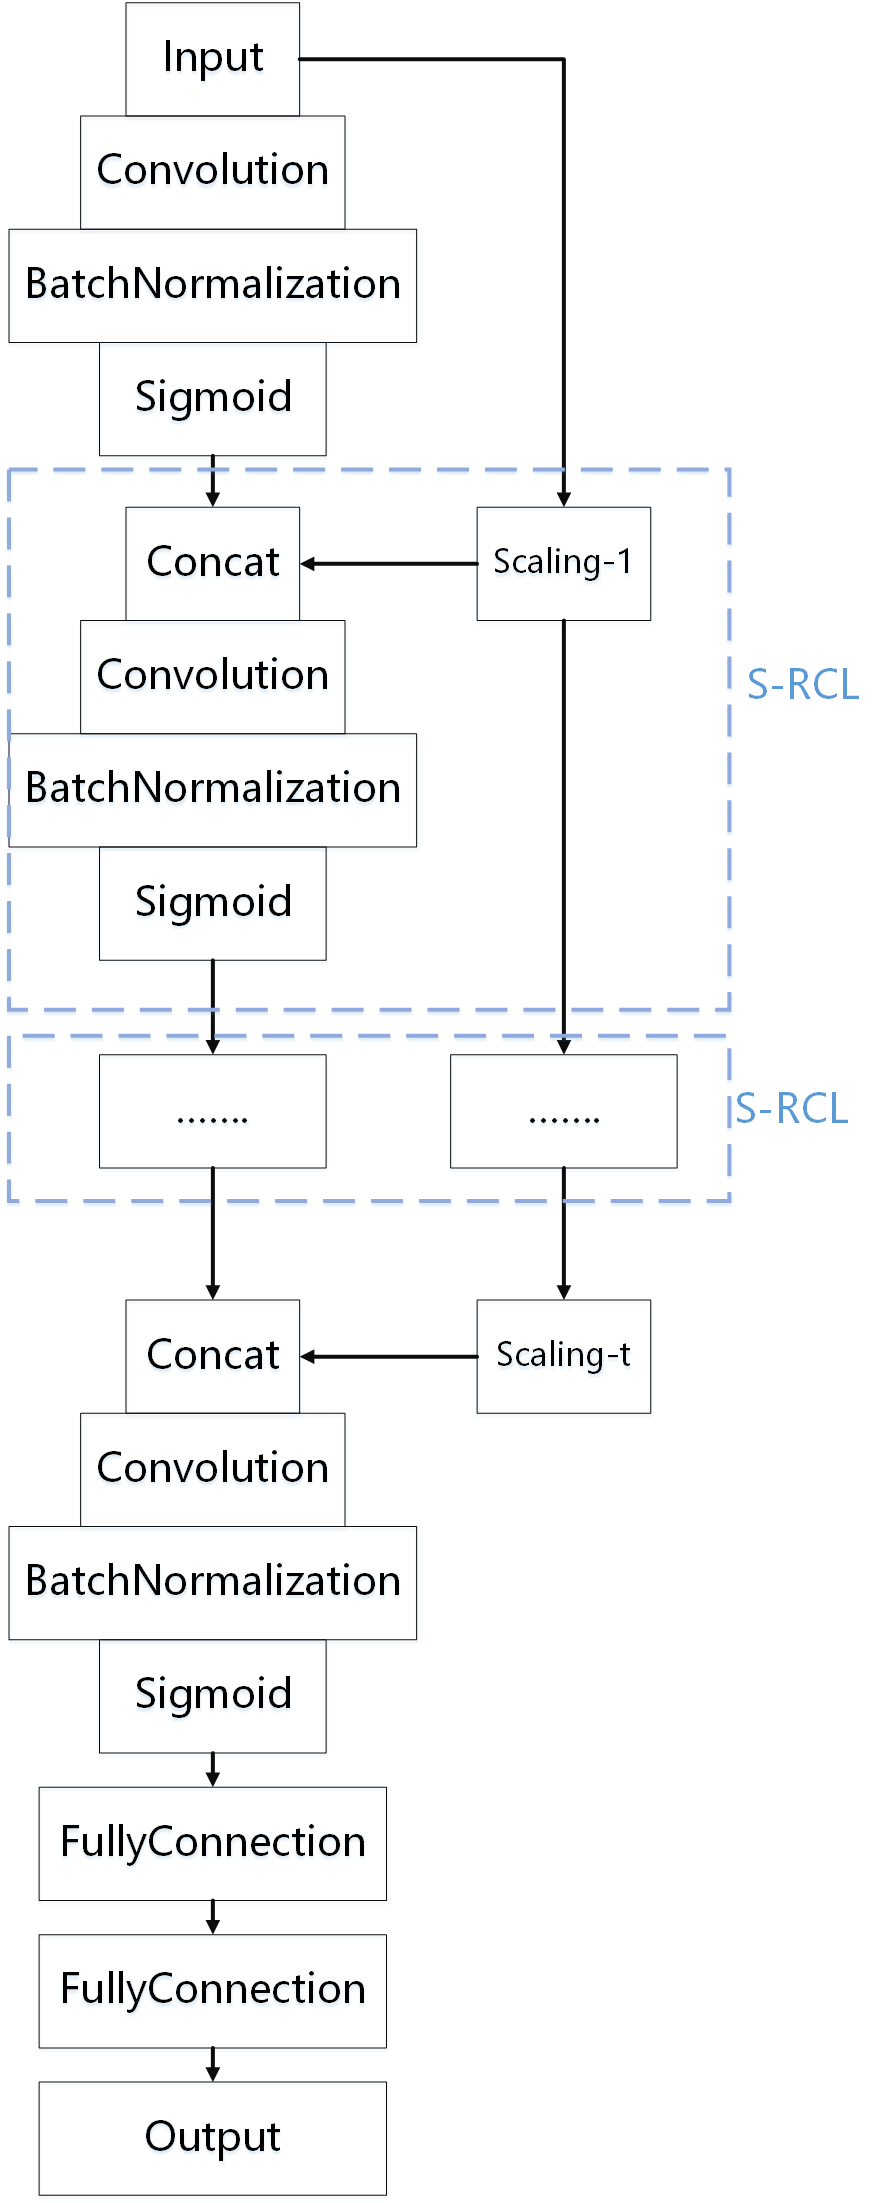
\includegraphics[width = 2in]{RCNN模型框架.png}
		\end{minipage}
	}
	\subfigure[Dense-S-RCNN连接结构]{
		\begin{minipage}[t]{0.4\linewidth}
			\centering
			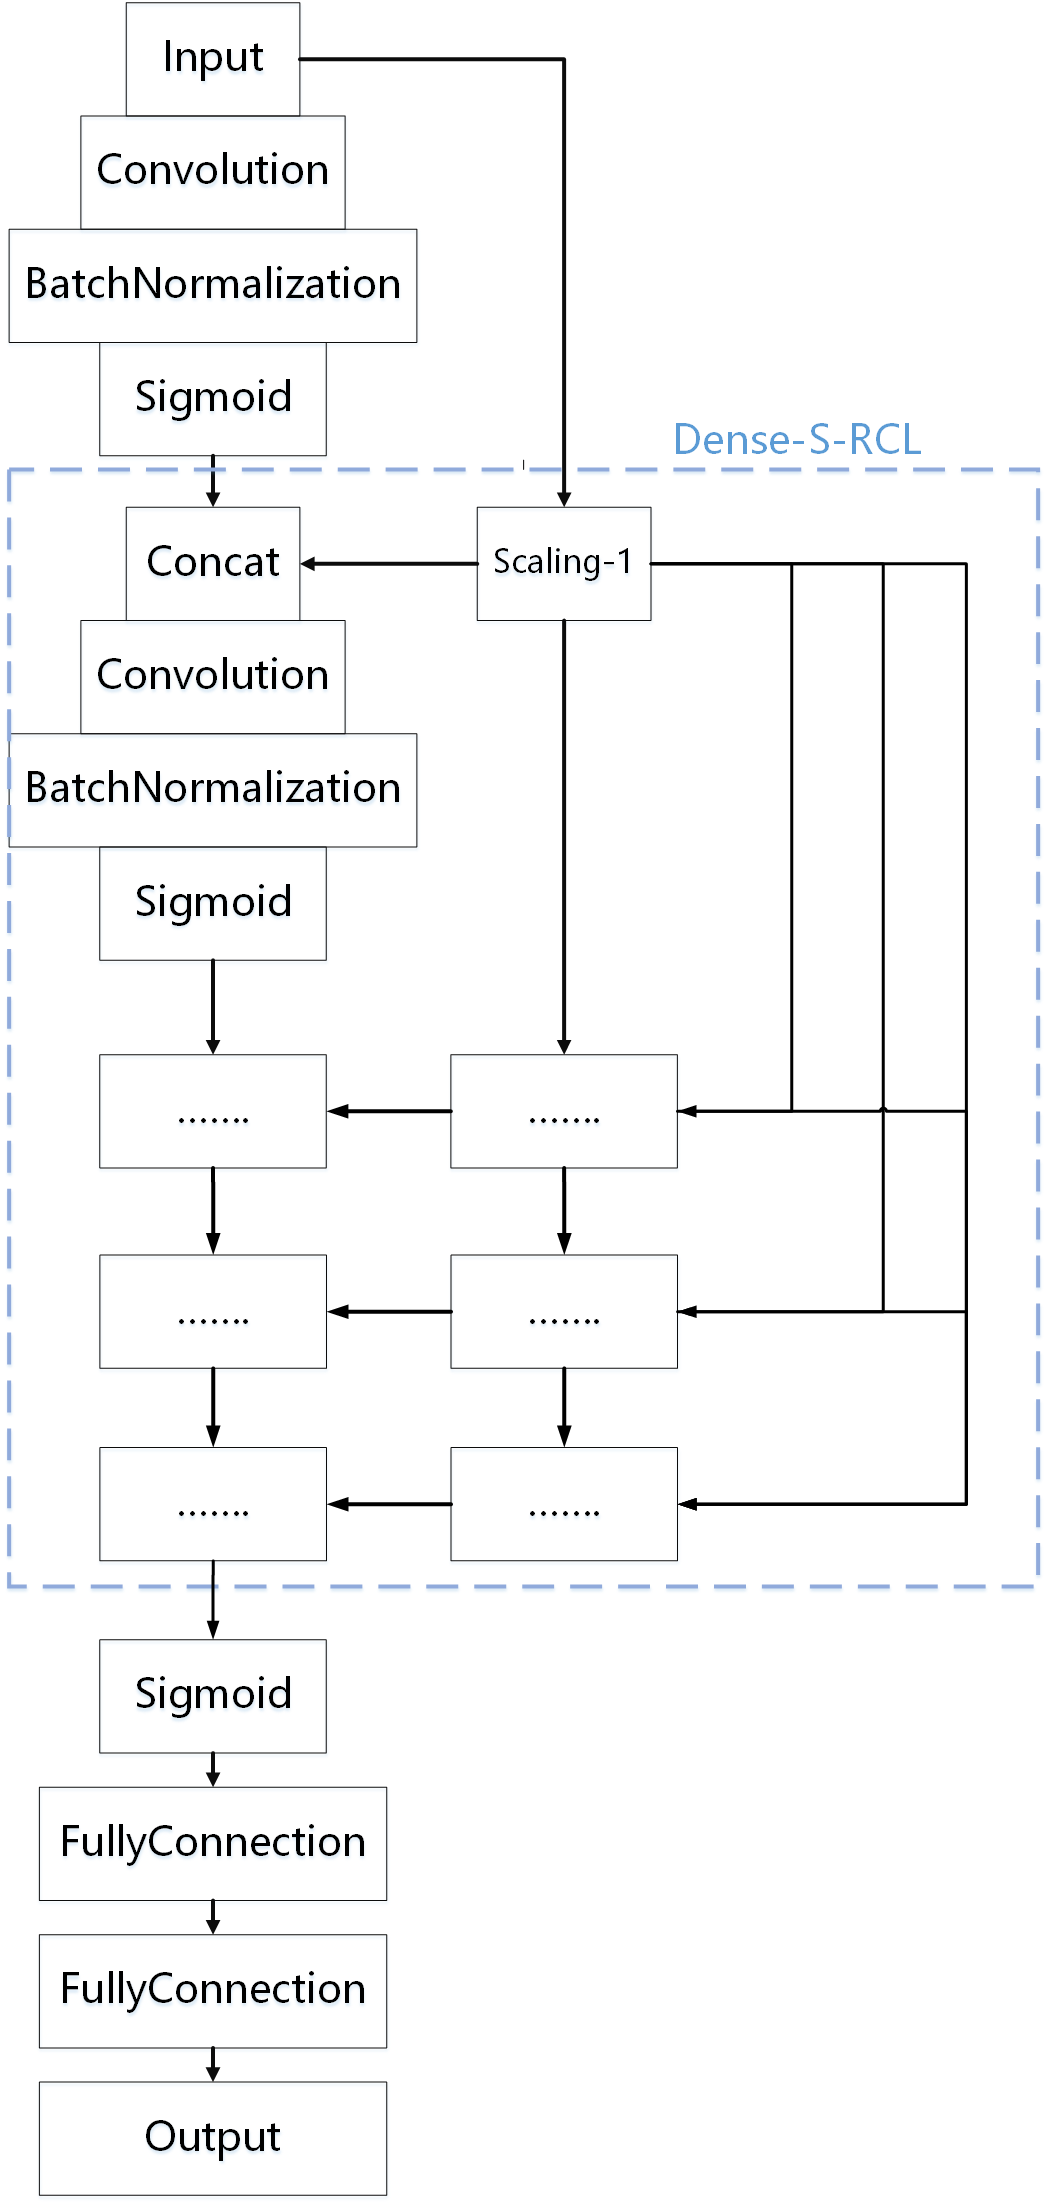
\includegraphics[width = 2.5in]{block.png}
		\end{minipage}
	}
	\caption{基于密集连接的多尺度特征金字塔对流初生检测模型架构}
	\label{RCNN_model}
\end{figure}

\backmatter
% !TEX root = ../main.tex

% 结论
\begin{conclusions}

    % 学位论文的结论作为论文正文的最后一章单独排写,但不加章标题序号。
    
    % 结论应是作者在学位论文研究过程中所取得的创新性成果的概要总结,不能与摘要混为一谈。博士学位论文结论应包括论文的主要结果、创新点、展望三部分,在结论中应概括论文的核心观点,明确、客观地指出本研究内容的创新性成果(含新见解、新观点、方法创新、技术创新、理论创新),并指出今后进一步在本研究方向进行研究工作的展望与设想。对所取得的创新性成果应注意从定性和定量两方面给出科学、准确的评价,分(1)、(2)、(3)…条列出,宜用“提出了”、“建立了”等词叙述。
    时间序列异常检测是工业界中一个重要的研究领域。尤其随着近年来工业4.0概念的提出,越来越多的行业提倡数字化,智能化,这激增了海量的时间序列数据。时间序列异常检测吸引了越来越多的研究者的关注,近年来有诸多学者提出了非常多的多元时间序列异常检测的算法及模型。然而这些方法都是都是面向完整的时间序列数据进行异常检测任务,然而在真实时间中多元时间序列往往包含着大量的缺失值。例如在工业场景中常常因为数据采集不全,传感器损坏等诸多因素所导致时间序列中包含缺失值。故本文课题为缺失值场景下的多元时间序列异常检测,按照填充-检测和不填充-检测的两种思路对包含缺失值的多元时间序列异常检测任务进行了如下研究:
    
    (1)按照填充-检测的思路,本文首先提出了一种基于对抗生成网络的填充算法,并对填充后的多元时间序列进行异常检测。较好的解决缺失值场景下的多元时间序列异常检测任务。本方法通过与多个基线模型对比,在完整数据集上,本章F1分数超过了第二名的基线0.3\%在缺失30\%数据的场景下F1分数超过了第二名的基线3\%,在缺失50\%数据的场景下F1分数超过了第二名的基线5\%。证明了我们的算法在缺失值场景的有效性。
    
    (2)考虑到在填充-检测的解决方案中,模型在训练时需要同时包含缺失值的时间序列和不包含缺失值的时间序列进行学习。这对数据的要求较高,在现实应用中实现难度较大。填充-检测的思路方案依然不能完美的解决缺失值多元时间序列异常检测问题。故本文提出了一种不填充-检测思路的多元时间序列异常检测方案,其基于注意力机制对缺失值时间序列进行重新表征,将不完整的多元时间序列重新表征为完整的高维表征,进而通过对该表征进行异常检测,更鲁棒的解决缺失值场景下的异常检测任务。本方法在三个常用经典时间序列数据集上进行的实验表明,该方法在缺失值场景下对比传统时间序列异常检测方法效果更好。最后,本文通过消融实验验证了各模块的有效性。
    
    本文的研究工作仍然存在着一定不足。例如当前异常检测的数据源过于单一,本文所提出的方法只能识别时间序列中的异常。 未来可以考虑引入多任务学习框架来联合现实世界中日志,图片等信息共同完成异常检测。同时,本文的异常检测模型在可解释性方面不足,未来可考虑引入根因分析模块以提高模型的可解释性帮助使用者完成根因定位。
    
    \end{conclusions}
       % 结论
% \bibliographystyle{hithesis} %如果没有参考文献时候
\bibliography{reference}
%%%%%%%%%%%%%%%%%%%%%%%%%%%%%%%%%%%%%%%%%%%%%%%%%%%%%%%%%%%%%%%%%%%%%%%%%%%%%%%% 
%-- 注意:以下本硕博、博后书序不一致 --%
%%%%%%%%%%%%%%%%%%%%%%%%%%%%%%%%%%%%%%%%%%%%%%%%%%%%%%%%%%%%%%%%%%%%%%%%%%%%%%%% 
%硕博书序
%%%%%%%%%%%%%%%%%%%%%%%%%%%%%%%%%%%%%%%%%%%%%%%%%%%%%%%%%%%%%%%%%%%%%%%%%%%%%%%% 
% \begin{appendix}%附录
%% -*-coding: utf-8 -*-
%%%%%%%%%%%%%%%%%%%%%%%%%%%%%%%%%%%%%%%%%%%%%%%%%%%%%%%%%
\chapter{带章节的附录}[Full Appendix]%
完整的附录内容,包含章节,公式,图表等

%%%%%%%%%%%%%%%%%%%%%%%%%%%%%%%%%%%%%%%%%%%%%%%%%%%%%%%%%
\section{附录节的内容}[Section in Appendix]
这是附录的节的内容

附录中图的示例:
\begin{figure}[htbp]
\centering
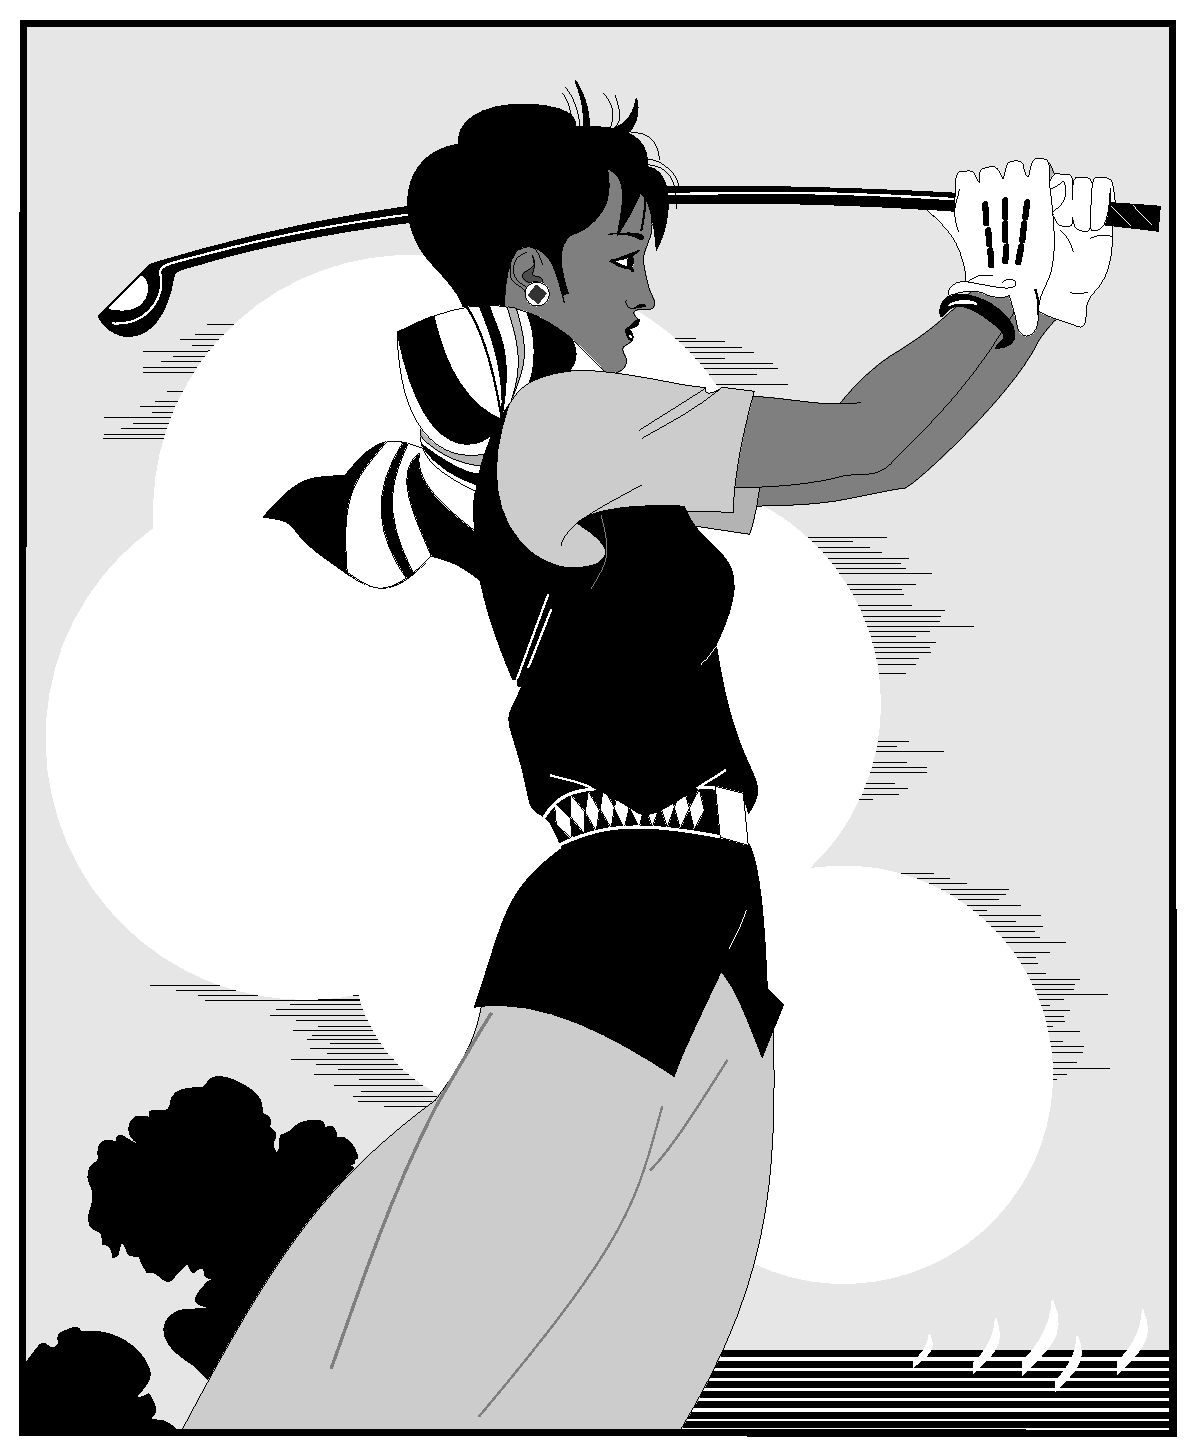
\includegraphics[width = 0.4\textwidth]{golfer}
%\bicaption[golfer5]{}{\xiaosi[0]打高尔夫球的人}{Fig.$\!$}{The person playing golf}\vspace{-1em}
\caption{\xiaosi[0]打高尔夫球的人}
\end{figure}

附录中公式的示例:
\begin{align}
a & = b \times c \\
E & = m c^2
\label{eq}
\end{align}

\chapter{这个星球上最好的免费Linux软件列表}[List of the Best Linux Software in our Planet]
\section{系统}

\href{http://fvwm.org/}{FVWM自从上世纪诞生以来,此星球最强大的窗口管理器。}
推荐基于FVWM的桌面设计hifvwm:\href{https://github.com/dustincys/hifvwm}{https://github.com/dustincys/hifvwm}。

\subsection{hifvwm的优点}

\begin{enumerate}
	\item 即使打开上百个窗口也不会“蒙圈”,对比win或mac都无法做到。计算机性能越来越强大,窗口任务的管理必须要升级到打怪兽级别。
	\item 二维可视化任务栏。
	\item 自动同步Bing搜索主页的壁纸。每次电脑开机,午夜零点自动更新,用户
		也可以手动更新,从此审美再也不疲劳。
	\item 切换窗口自动聚焦到最上面的窗口。使用键盘快捷键切换窗口时候,减少
		操作过程,自动聚焦到目标窗口。这一特性是虚拟窗口必须的人性化设
		计。
	\item 类似window右下角的功能的最小化窗口来显示桌面的功能此处类似
		win7/win10,实现在一个桌面之内操作多个任务。
	\item 任务栏结合标题栏。采用任务栏和标题栏结合,节省空间。
	\item 同类窗口切换。可以在同类窗口之内类似alt-tab的方式切换。
	\item ……
\end{enumerate}

\section{其他}

\href{https://github.com/goldendict/goldendict}{goldendict 星球最强大的桌面字典。}

\href{https://github.com/yarrick/iodine}{iodine,“HIT-WLAN + 锐捷”时代的福音。}

\href{http://www.aircrack-ng.org/}{aircrack,Wifi“安全性评估”工具,自由上网,
  就是隔壁寝室网络会变慢一点。}

\href{https://www.ledger-cli.org/}{ledger,前“金融区块链”时代最好的复式记账系统。}

\href{https://orgmode.org/}{orgmode,最强大的笔记系统,从来没有之一。}

\href{https://www.jianguoyun.com/}{坚果云,国内一款支持WebDav的云盘系统,国内真正的云盘没有之一。}

\href{https://notmuchmail.org/}{notmuch, 目前最好的邮件管理工具,还在为每天几百
  个email苦恼?几百个这些都不算多,notmuch。}

\section{vim}
实现中英文每一句一行,以及实现每一句折叠断行的简单正则式,tex源码更加乖乖。
\begin{lstlisting}
vnoremap <leader>fae J:s/[.!?]\zs\s\+/\="\r".matchstr(getline('.'), '^\s*')/g<CR>
vnoremap <leader>fac J:s/[。!?]/\=submatch(0)."\n".matchstr(getline('.'), '^\s*')/g<CR>
vnoremap <leader>fle :!fmt -80 -s<CR>
\end{lstlisting}

% \end{appendix}
% !Mode:: "TeX:UTF-8" 
\begin{publication}
% \noindent\textbf{发表的相关论文}
% \begin{publist}
% \item	XXX,XXX. Static Oxidation Model of Al-Mg/C Dissipation Thermal Protection Materials[J]. Rare Metal Materials and Engineering, 2010, 39(Suppl. 1): 520-524.(SCI~收录,IDS号为~669JS,IF=0.16)
% \item XXX,XXX. 精密超声振动切削单晶铜的计算机仿真研究[J]. 系统仿真学报,2007,19(4):738-741,753.(EI~收录号:20071310514841)
% \item XXX,XXX. 局部多孔质气体静压轴向轴承静态特性的数值求解[J]. 摩擦学学报,2007(1):68-72.(EI~收录号:20071510544816)
% \item XXX,XXX. 硬脆光学晶体材料超精密切削理论研究综述[J]. 机械工程学报,2003,39(8):15-22.(EI~收录号:2004088028875)
% \item XXX,XXX. 基于遗传算法的超精密切削加工表面粗糙度预测模型的参数辨识以及切削参数优化[J]. 机械工程学报,2005,41(11):158-162.(EI~收录号:2006039650087)
% \item XXX,XXX. Discrete Sliding Mode Cintrok with Fuzzy Adaptive Reaching Law on 6-PEES Parallel Robot[C]. Intelligent System Design and Applications, Jinan, 2006: 649-652.(EI~收录号:20073210746529)
% \end{publist} 

\noindent\textbf{申请及已获得的专利}
\begin{publist}
\item 廖清,曾子辉,柴合言,苏伟俊,刘洋,蒋琳,王轩. 一种面向多种类数据的异常检测方法及装置:中国,CN111580979A[P]. 2021.
\end{publist}

% \noindent\textbf{比赛获奖}
% \begin{publist}
% \item 2020年第八届CCF大数据与计算智能大赛,大数据时代的Serverless工作负载预测赛题,队长谢志彬,队员聂才、傅鲲阳、李唯一,排名:8/2404 
% % \item	XXX,XXX. XX~气体静压轴承技术研究, XX~省自然科学基金项目.课题编号:XXXX.
% % \item XXX,XXX. XX~静载下预应力混凝土房屋结构设计统一理论. 黑江省科学技术二等奖, 2007.
% \end{publist}
% \vfill
% \hangafter=1\hangindent=2em\noindent
% %\setlength{\parindent}{2em}

\end{publication}
    % 所发文章
%\begin{ceindex}
  %如果想要手动加索引,注释掉以下这一样,用wordlist环境
\printsubindex*
\end{ceindex}
    % 索引, 根据自己的情况添加或者不添加,选择自动添加或者手工添加。
\authorization %授权
%\authorization[saomiao.pdf] %添加扫描页的命令,与上互斥
\begin{acknowledgements}
    时光飞逝。硕士研究生生活即将结束,两年半的学习生活使我受益匪浅。经历了大半年时间的收集与整理、汇编,我深深体会到了写作论文时的那份宁静与思考。回首两年半的求学历程,对那些引导我、帮助我、激励我的人,心中充满了感激。

    首先要感谢导师廖清老师,论文定题到写作定稿,倾注了廖老师大量的心血。在论文的选题、搜集资料和写作等阶段,廖老师都倾注了极大的关怀和鼓励。在我初稿完成之后,廖老师又在百忙之中抽出空来对我的论文认真的批改,指点迷津,提出许多中肯的指导意见,使我在研究和写作过程中不致迷失方向。借此机会,谨向廖老师表示我最诚挚的敬意和感谢!
    
    其次,要感谢学校的老师,正是因为有了他们严格、无私、高质量的教导,我才能在这几年的学习过程中汲取专业知识和迅速提升能力;同时也感谢这三年来与我互勉互励的诸位同学,感谢我的同门:张瑞淇,黄裕涛,莫重;感谢我的室友:朱焱,吴凯涛,文耀军;在各位同学的共同努力之下,我们始终拥有一个良好的生活环境和一个积极向上的学习氛围,能在这样一个团队中度过,是我极大的荣幸.感谢一直关心与支持我的同学和朋友们!
    
    最后,还要特别感谢培养我长大含辛茹苦的父母和在我面临人生选择迷茫之际为我排忧解难的兄弟姐妹们,谢谢你们!
    
    在校的学习生活让我更能够明确今后的发展方向,学校老师对我的帮助是一笔无价的财富。我将在今后的工作、学习中加倍努力,以期能够取得更多成果回报你们、回报社会。再次感谢你们,祝你们一生幸福、安康!

\end{acknowledgements}
 %致谢
%% !Mode:: "TeX:UTF-8" 

\begin{resume}
1996~年~08~月~31~日出生于~河北保定。

2015~年~09~月考入~南开~大学~计算机~院(系)计算机科学与技术~专业,2019~年~06~月本科毕业并获得~工~学学士学位。

2019~年~09~月------2022~年~01~月在~哈尔滨工业大学(深圳)~计算机科学与技术~学院 计算机技术专业学习并获得~XX~学硕士学位。


\end{resume}
          % 博士学位论文有个人简介
%%%%%%%%%%%%%%%%%%%%%%%%%%%%%%%%%%%%%%%%%%%%%%%%%%%%%%%%%%%%%%%%%%%%%%%%%%%%%%%% 
%本科书序为:
%%%%%%%%%%%%%%%%%%%%%%%%%%%%%%%%%%%%%%%%%%%%%%%%%%%%%%%%%%%%%%%%%%%%%%%%%%%%%%%% 
% \authorization %授权
% % \authorization[saomiao.pdf] %添加扫描页的命令,与上互斥
% \begin{acknowledgements}
    时光飞逝。硕士研究生生活即将结束,两年半的学习生活使我受益匪浅。经历了大半年时间的收集与整理、汇编,我深深体会到了写作论文时的那份宁静与思考。回首两年半的求学历程,对那些引导我、帮助我、激励我的人,心中充满了感激。

    首先要感谢导师廖清老师,论文定题到写作定稿,倾注了廖老师大量的心血。在论文的选题、搜集资料和写作等阶段,廖老师都倾注了极大的关怀和鼓励。在我初稿完成之后,廖老师又在百忙之中抽出空来对我的论文认真的批改,指点迷津,提出许多中肯的指导意见,使我在研究和写作过程中不致迷失方向。借此机会,谨向廖老师表示我最诚挚的敬意和感谢!
    
    其次,要感谢学校的老师,正是因为有了他们严格、无私、高质量的教导,我才能在这几年的学习过程中汲取专业知识和迅速提升能力;同时也感谢这三年来与我互勉互励的诸位同学,感谢我的同门:张瑞淇,黄裕涛,莫重;感谢我的室友:朱焱,吴凯涛,文耀军;在各位同学的共同努力之下,我们始终拥有一个良好的生活环境和一个积极向上的学习氛围,能在这样一个团队中度过,是我极大的荣幸.感谢一直关心与支持我的同学和朋友们!
    
    最后,还要特别感谢培养我长大含辛茹苦的父母和在我面临人生选择迷茫之际为我排忧解难的兄弟姐妹们,谢谢你们!
    
    在校的学习生活让我更能够明确今后的发展方向,学校老师对我的帮助是一笔无价的财富。我将在今后的工作、学习中加倍努力,以期能够取得更多成果回报你们、回报社会。再次感谢你们,祝你们一生幸福、安康!

\end{acknowledgements}
 %致谢
% \begin{appendix}%附录
% \chapter{外文资料原文}
\label{cha:engorg}

\title{The title of the English paper}

\textbf{Abstract:} As one of the most widely used techniques in operations
research, \emph{ mathematical programming} is defined as a means of maximizing a
quantity known as \emph{bjective function}, subject to a set of constraints
represented by equations and inequalities. Some known subtopics of mathematical
programming are linear programming, nonlinear programming, multiobjective
programming, goal programming, dynamic programming, and multilevel
programming$^{[1]}$.

It is impossible to cover in a single chapter every concept of mathematical
programming. This chapter introduces only the basic concepts and techniques of
mathematical programming such that readers gain an understanding of them
throughout the book$^{[2,3]}$.


\section{Single-Objective Programming}
The general form of single-objective programming (SOP) is written
as follows,
\begin{equation}\tag*{(123)} % 如果附录中的公式不想让它出现在公式索引中,那就请
                             % 用 \tag*{xxxx}
\left\{\begin{array}{l}
\max \,\,f(x)\\[0.1 cm]
\mbox{subject to:} \\ [0.1 cm]
\qquad g_j(x)\le 0,\quad j=1,2,\cdots,p
\end{array}\right.
\end{equation}
which maximizes a real-valued function $f$ of
$x=(x_1,x_2,\cdots,x_n)$ subject to a set of constraints.

\newtheorem{mpdef}{Definition}[chapter]
\begin{mpdef}
In SOP, we call $x$ a decision vector, and
$x_1,x_2,\cdots,x_n$ decision variables. The function
$f$ is called the objective function. The set
\begin{equation}\tag*{(456)} % 这里同理,其它不再一一指定。
S=\left\{x\in\Re^n\bigm|g_j(x)\le 0,\,j=1,2,\cdots,p\right\}
\end{equation}
is called the feasible set. An element $x$ in $S$ is called a
feasible solution.
\end{mpdef}

\newtheorem{mpdefop}[mpdef]{Definition}
\begin{mpdefop}
A feasible solution $x^*$ is called the optimal
solution of SOP if and only if
\begin{equation}
f(x^*)\ge f(x)
\end{equation}
for any feasible solution $x$.
\end{mpdefop}

One of the outstanding contributions to mathematical programming was known as
the Kuhn-Tucker conditions\ref{eq:ktc}. In order to introduce them, let us give
some definitions. An inequality constraint $g_j(x)\le 0$ is said to be active at
a point $x^*$ if $g_j(x^*)=0$. A point $x^*$ satisfying $g_j(x^*)\le 0$ is said
to be regular if the gradient vectors $\nabla g_j(x)$ of all active constraints
are linearly independent.

Let $x^*$ be a regular point of the constraints of SOP and assume that all the
functions $f(x)$ and $g_j(x),j=1,2,\cdots,p$ are differentiable. If $x^*$ is a
local optimal solution, then there exist Lagrange multipliers
$\lambda_j,j=1,2,\cdots,p$ such that the following Kuhn-Tucker conditions hold,
\begin{equation}
\label{eq:ktc}
\left\{\begin{array}{l}
    \nabla f(x^*)-\sum\limits_{j=1}^p\lambda_j\nabla g_j(x^*)=0\\[0.3cm]
    \lambda_jg_j(x^*)=0,\quad j=1,2,\cdots,p\\[0.2cm]
    \lambda_j\ge 0,\quad j=1,2,\cdots,p.
\end{array}\right.
\end{equation}
If all the functions $f(x)$ and $g_j(x),j=1,2,\cdots,p$ are convex and
differentiable, and the point $x^*$ satisfies the Kuhn-Tucker conditions
(\ref{eq:ktc}), then it has been proved that the point $x^*$ is a global optimal
solution of SOP.

\subsection{Linear Programming}
\label{sec:lp}

If the functions $f(x),g_j(x),j=1,2,\cdots,p$ are all linear, then SOP is called
a {\em linear programming}.

The feasible set of linear is always convex. A point $x$ is called an extreme
point of convex set $S$ if $x\in S$ and $x$ cannot be expressed as a convex
combination of two points in $S$. It has been shown that the optimal solution to
linear programming corresponds to an extreme point of its feasible set provided
that the feasible set $S$ is bounded. This fact is the basis of the {\em simplex
  algorithm} which was developed by Dantzig as a very efficient method for
solving linear programming.
\begin{table}[ht]
\centering
  \centering
  \caption*{Table~1\hskip1em This is an example for manually numbered table, which
    would not appear in the list of tables}
  \label{tab:badtabular2}
  \begin{tabular}[c]{|m{1.5cm}|c|c|c|c|c|c|}\hline
    \multicolumn{2}{|c|}{Network Topology} & \# of nodes &
    \multicolumn{3}{c|}{\# of clients} & Server \\\hline
    GT-ITM & Waxman Transit-Stub & 600 &
    \multirow{2}{2em}{2\%}&
    \multirow{2}{2em}{10\%}&
    \multirow{2}{2em}{50\%}&
    \multirow{2}{1.2in}{Max. Connectivity}\\\cline{1-3}
    \multicolumn{2}{|c|}{Inet-2.1} & 6000 & & & &\\\hline
    & \multicolumn{2}{c|}{ABCDEF} &\multicolumn{4}{c|}{} \\\hline
\end{tabular}
\end{table}

Roughly speaking, the simplex algorithm examines only the extreme points of the
feasible set, rather than all feasible points. At first, the simplex algorithm
selects an extreme point as the initial point. The successive extreme point is
selected so as to improve the objective function value. The procedure is
repeated until no improvement in objective function value can be made. The last
extreme point is the optimal solution.

\subsection{Nonlinear Programming}

If at least one of the functions $f(x),g_j(x),j=1,2,\cdots,p$ is nonlinear, then
SOP is called a {\em nonlinear programming}.

A large number of classical optimization methods have been developed to treat
special-structural nonlinear programming based on the mathematical theory
concerned with analyzing the structure of problems.

Now we consider a nonlinear programming which is confronted solely with
maximizing a real-valued function with domain $\Re^n$.  Whether derivatives are
available or not, the usual strategy is first to select a point in $\Re^n$ which
is thought to be the most likely place where the maximum exists. If there is no
information available on which to base such a selection, a point is chosen at
random. From this first point an attempt is made to construct a sequence of
points, each of which yields an improved objective function value over its
predecessor. The next point to be added to the sequence is chosen by analyzing
the behavior of the function at the previous points. This construction continues
until some termination criterion is met. Methods based upon this strategy are
called {\em ascent methods}, which can be classified as {\em direct methods},
{\em gradient methods}, and {\em Hessian methods} according to the information
about the behavior of objective function $f$. Direct methods require only that
the function can be evaluated at each point. Gradient methods require the
evaluation of first derivatives of $f$. Hessian methods require the evaluation
of second derivatives. In fact, there is no superior method for all
problems. The efficiency of a method is very much dependent upon the objective
function.

\subsection{Integer Programming}

{\em Integer programming} is a special mathematical programming in which all of
the variables are assumed to be only integer values. When there are not only
integer variables but also conventional continuous variables, we call it {\em
  mixed integer programming}. If all the variables are assumed either 0 or 1,
then the problem is termed a {\em zero-one programming}. Although integer
programming can be solved by an {\em exhaustive enumeration} theoretically, it
is impractical to solve realistically sized integer programming problems. The
most successful algorithm so far found to solve integer programming is called
the {\em branch-and-bound enumeration} developed by Balas (1965) and Dakin
(1965). The other technique to integer programming is the {\em cutting plane
  method} developed by Gomory (1959).

\hfill\textit{Uncertain Programming\/}\quad(\textsl{BaoDing Liu, 2006.2})

\section*{References}
\noindent{\itshape NOTE: These references are only for demonstration. They are
  not real citations in the original text.}

\begin{translationbib}
\item Donald E. Knuth. The \TeX book. Addison-Wesley, 1984. ISBN: 0-201-13448-9
\item Paul W. Abrahams, Karl Berry and Kathryn A. Hargreaves. \TeX\ for the
  Impatient. Addison-Wesley, 1990. ISBN: 0-201-51375-7
\item David Salomon. The advanced \TeX book.  New York : Springer, 1995. ISBN:0-387-94556-3
\end{translationbib}

\chapter{外文资料的调研阅读报告或书面翻译}

\title{英文资料的中文标题}

{\heiti 摘要:} 本章为外文资料翻译内容。如果有摘要可以直接写上来,这部分好像没有
明确的规定。

\section{单目标规划}
北冥有鱼,其名为鲲。鲲之大,不知其几千里也。化而为鸟,其名为鹏。鹏之背,不知其几
千里也。怒而飞,其翼若垂天之云。是鸟也,海运则将徙于南冥。南冥者,天池也。
\begin{equation}\tag*{(123)}
 p(y|\mathbf{x}) = \frac{p(\mathbf{x},y)}{p(\mathbf{x})}=
\frac{p(\mathbf{x}|y)p(y)}{p(\mathbf{x})}
\end{equation}

吾生也有涯,而知也无涯。以有涯随无涯,殆已!已而为知者,殆而已矣!为善无近名,为
恶无近刑,缘督以为经,可以保身,可以全生,可以养亲,可以尽年。

\subsection{线性规划}
庖丁为文惠君解牛,手之所触,肩之所倚,足之所履,膝之所倚,砉然响然,奏刀騞然,莫
不中音,合于桑林之舞,乃中经首之会。
\begin{table}[ht]
\centering
  \centering
  \caption*{表~1\hskip1em 这是手动编号但不出现在索引中的一个表格例子}
  \label{tab:badtabular3}
  \begin{tabular}[c]{|m{1.5cm}|c|c|c|c|c|c|}\hline
    \multicolumn{2}{|c|}{Network Topology} & \# of nodes &
    \multicolumn{3}{c|}{\# of clients} & Server \\\hline
    GT-ITM & Waxman Transit-Stub & 600 &
    \multirow{2}{2em}{2\%}&
    \multirow{2}{2em}{10\%}&
    \multirow{2}{2em}{50\%}&
    \multirow{2}{1.2in}{Max. Connectivity}\\\cline{1-3}
    \multicolumn{2}{|c|}{Inet-2.1} & 6000 & & & &\\\hline
    & \multicolumn{2}{c|}{ABCDEF} &\multicolumn{4}{c|}{} \\\hline
\end{tabular}
\end{table}

文惠君曰:“嘻,善哉!技盖至此乎?”庖丁释刀对曰:“臣之所好者道也,进乎技矣。始臣之
解牛之时,所见无非全牛者;三年之后,未尝见全牛也;方今之时,臣以神遇而不以目视,
官知止而神欲行。依乎天理,批大郤,导大窾,因其固然。技经肯綮之未尝,而况大坬乎!
良庖岁更刀,割也;族庖月更刀,折也;今臣之刀十九年矣,所解数千牛矣,而刀刃若新发
于硎。彼节者有间而刀刃者无厚,以无厚入有间,恢恢乎其于游刃必有余地矣。是以十九年
而刀刃若新发于硎。虽然,每至于族,吾见其难为,怵然为戒,视为止,行为迟,动刀甚微,
謋然已解,如土委地。提刀而立,为之而四顾,为之踌躇满志,善刀而藏之。”

文惠君曰:“善哉!吾闻庖丁之言,得养生焉。”


\subsection{非线性规划}
孔子与柳下季为友,柳下季之弟名曰盗跖。盗跖从卒九千人,横行天下,侵暴诸侯。穴室枢
户,驱人牛马,取人妇女。贪得忘亲,不顾父母兄弟,不祭先祖。所过之邑,大国守城,小
国入保,万民苦之。孔子谓柳下季曰:“夫为人父者,必能诏其子;为人兄者,必能教其弟。
若父不能诏其子,兄不能教其弟,则无贵父子兄弟之亲矣。今先生,世之才士也,弟为盗
跖,为天下害,而弗能教也,丘窃为先生羞之。丘请为先生往说之。”

柳下季曰:“先生言为人父者必能诏其子,为人兄者必能教其弟,若子不听父之诏,弟不受
兄之教,虽今先生之辩,将奈之何哉?且跖之为人也,心如涌泉,意如飘风,强足以距敌,
辩足以饰非。顺其心则喜,逆其心则怒,易辱人以言。先生必无往。”

孔子不听,颜回为驭,子贡为右,往见盗跖。

\subsection{整数规划}
盗跖乃方休卒徒大山之阳,脍人肝而餔之。孔子下车而前,见谒者曰:“鲁人孔丘,闻将军
高义,敬再拜谒者。”谒者入通。盗跖闻之大怒,目如明星,发上指冠,曰:“此夫鲁国之
巧伪人孔丘非邪?为我告之:尔作言造语,妄称文、武,冠枝木之冠,带死牛之胁,多辞缪
说,不耕而食,不织而衣,摇唇鼓舌,擅生是非,以迷天下之主,使天下学士不反其本,妄
作孝弟,而侥幸于封侯富贵者也。子之罪大极重,疾走归!不然,我将以子肝益昼餔之膳。”


\chapter{其它附录}
前面两个附录主要是给本科生做例子。其它附录的内容可以放到这里,当然如果你愿意,可
以把这部分也放到独立的文件中,然后将其到主文件中。
%本科生翻译论文
% \end{appendix}
%%%%%%%%%%%%%%%%%%%%%%%%%%%%%%%%%%%%%%%%%%%%%%%%%%%%%%%%%%%%%%%%%%%%%%%%%%%%%%%% 
% 博后书序
%%%%%%%%%%%%%%%%%%%%%%%%%%%%%%%%%%%%%%%%%%%%%%%%%%%%%%%%%%%%%%%%%%%%%%%%%%%%%%%% 
% \begin{acknowledgements}
    时光飞逝。硕士研究生生活即将结束,两年半的学习生活使我受益匪浅。经历了大半年时间的收集与整理、汇编,我深深体会到了写作论文时的那份宁静与思考。回首两年半的求学历程,对那些引导我、帮助我、激励我的人,心中充满了感激。

    首先要感谢导师廖清老师,论文定题到写作定稿,倾注了廖老师大量的心血。在论文的选题、搜集资料和写作等阶段,廖老师都倾注了极大的关怀和鼓励。在我初稿完成之后,廖老师又在百忙之中抽出空来对我的论文认真的批改,指点迷津,提出许多中肯的指导意见,使我在研究和写作过程中不致迷失方向。借此机会,谨向廖老师表示我最诚挚的敬意和感谢!
    
    其次,要感谢学校的老师,正是因为有了他们严格、无私、高质量的教导,我才能在这几年的学习过程中汲取专业知识和迅速提升能力;同时也感谢这三年来与我互勉互励的诸位同学,感谢我的同门:张瑞淇,黄裕涛,莫重;感谢我的室友:朱焱,吴凯涛,文耀军;在各位同学的共同努力之下,我们始终拥有一个良好的生活环境和一个积极向上的学习氛围,能在这样一个团队中度过,是我极大的荣幸.感谢一直关心与支持我的同学和朋友们!
    
    最后,还要特别感谢培养我长大含辛茹苦的父母和在我面临人生选择迷茫之际为我排忧解难的兄弟姐妹们,谢谢你们!
    
    在校的学习生活让我更能够明确今后的发展方向,学校老师对我的帮助是一笔无价的财富。我将在今后的工作、学习中加倍努力,以期能够取得更多成果回报你们、回报社会。再次感谢你们,祝你们一生幸福、安康!

\end{acknowledgements}
 %致谢
% % !Mode:: "TeX:UTF-8" 

\begin{doctorpublication}
\noindent\textbf{(一)发表的学术论文}
\begin{publist}
\item	XXX,XXX. Static Oxidation Model of Al-Mg/C Dissipation Thermal Protection Materials[J]. Rare Metal Materials and Engineering, 2010, 39(Suppl. 1): 520-524.(SCI~收录,IDS号为~669JS,IF=0.16)
\item XXX,XXX. 精密超声振动切削单晶铜的计算机仿真研究[J]. 系统仿真学报,2007,19(4):738-741,753.(EI~收录号:20071310514841)
\item XXX,XXX. 局部多孔质气体静压轴向轴承静态特性的数值求解[J]. 摩擦学学报,2007(1):68-72.(EI~收录号:20071510544816)
\item XXX,XXX. 硬脆光学晶体材料超精密切削理论研究综述[J]. 机械工程学报,2003,39(8):15-22.(EI~收录号:2004088028875)
\item XXX,XXX. 基于遗传算法的超精密切削加工表面粗糙度预测模型的参数辨识以及切削参数优化[J]. 机械工程学报,2005,41(11):158-162.(EI~收录号:2006039650087)
\item XXX,XXX. Discrete Sliding Mode Cintrok with Fuzzy Adaptive Reaching Law on 6-PEES Parallel Robot[C]. Intelligent System Design and Applications, Jinan, 2006: 649-652.(EI~收录号:20073210746529)
\end{publist}

\noindent\textbf{(二)申请及已获得的专利(无专利时此项不必列出)}
\begin{publist}
\item XXX,XXX. 一种温热外敷药制备方案:中国,88105607.3[P]. 1989-07-26.
\end{publist}

\noindent\textbf{(三)参与的科研项目及获奖情况}
\begin{publist}
\item	XXX,XXX. XX~气体静压轴承技术研究, XX~省自然科学基金项目.课题编号:XXXX.
\item XXX,XXX. XX~静载下预应力混凝土房屋结构设计统一理论. 黑江省科学技术二等奖, 2007.
\end{publist}
%\vfill
%\hangafter=1\hangindent=2em\noindent
%\setlength{\parindent}{2em}
\end{doctorpublication}
    % 所发文章
% % !Mode:: "TeX:UTF-8" 
\begin{publication}
% \noindent\textbf{发表的相关论文}
% \begin{publist}
% \item	XXX,XXX. Static Oxidation Model of Al-Mg/C Dissipation Thermal Protection Materials[J]. Rare Metal Materials and Engineering, 2010, 39(Suppl. 1): 520-524.(SCI~收录,IDS号为~669JS,IF=0.16)
% \item XXX,XXX. 精密超声振动切削单晶铜的计算机仿真研究[J]. 系统仿真学报,2007,19(4):738-741,753.(EI~收录号:20071310514841)
% \item XXX,XXX. 局部多孔质气体静压轴向轴承静态特性的数值求解[J]. 摩擦学学报,2007(1):68-72.(EI~收录号:20071510544816)
% \item XXX,XXX. 硬脆光学晶体材料超精密切削理论研究综述[J]. 机械工程学报,2003,39(8):15-22.(EI~收录号:2004088028875)
% \item XXX,XXX. 基于遗传算法的超精密切削加工表面粗糙度预测模型的参数辨识以及切削参数优化[J]. 机械工程学报,2005,41(11):158-162.(EI~收录号:2006039650087)
% \item XXX,XXX. Discrete Sliding Mode Cintrok with Fuzzy Adaptive Reaching Law on 6-PEES Parallel Robot[C]. Intelligent System Design and Applications, Jinan, 2006: 649-652.(EI~收录号:20073210746529)
% \end{publist} 

\noindent\textbf{申请及已获得的专利}
\begin{publist}
\item 廖清,曾子辉,柴合言,苏伟俊,刘洋,蒋琳,王轩. 一种面向多种类数据的异常检测方法及装置:中国,CN111580979A[P]. 2021.
\end{publist}

% \noindent\textbf{比赛获奖}
% \begin{publist}
% \item 2020年第八届CCF大数据与计算智能大赛,大数据时代的Serverless工作负载预测赛题,队长谢志彬,队员聂才、傅鲲阳、李唯一,排名:8/2404 
% % \item	XXX,XXX. XX~气体静压轴承技术研究, XX~省自然科学基金项目.课题编号:XXXX.
% % \item XXX,XXX. XX~静载下预应力混凝土房屋结构设计统一理论. 黑江省科学技术二等奖, 2007.
% \end{publist}
% \vfill
% \hangafter=1\hangindent=2em\noindent
% %\setlength{\parindent}{2em}

\end{publication}
    % 所发文章
% % !Mode:: "TeX:UTF-8" 

\begin{resume}
1996~年~08~月~31~日出生于~河北保定。

2015~年~09~月考入~南开~大学~计算机~院(系)计算机科学与技术~专业,2019~年~06~月本科毕业并获得~工~学学士学位。

2019~年~09~月------2022~年~01~月在~哈尔滨工业大学(深圳)~计算机科学与技术~学院 计算机技术专业学习并获得~XX~学硕士学位。


\end{resume}
          % 博士学位论文有个人简介
% % !Mode:: "TeX:UTF-8"
\begin{correspondingaddr}
  \heiti\xiaosi
  \noindent 永久通讯地址: \par
  \noindent email: \par
  \noindent 电话: \par
\end{correspondingaddr}
 %通信地址
%%%%%%%%%%%%%%%%%%%%%%%%%%%%%%%%%%%%%%%%%%%%%%%%%%%%%%%%%%%%%%%%%%%%%%%%%%%%%%%% 
\end{document}
% Local Variables:
% TeX-engine: xetex
% End:
